\documentclass[10pt,twocolumn,letterpaper]{article}

\usepackage{cvpr}
\usepackage{times}
\usepackage{epsfig}
\usepackage{graphicx}
\usepackage{amsmath}
\usepackage{amssymb}
\usepackage{import}
\usepackage{subcaption}
% Necessary for sideways figures
\usepackage{rotating}
\usepackage{bm}

\linespread{0.992}

\newcommand{\bb}[1]{{\bm{#1}}}
\newcommand\MatTableStrut{\rule{0pt}{8ex}\rule[-8ex]{0pt}{0pt}}
\newcommand{\NC}[1]{{\textbf{\color{blue}[NC: #1]}}}
\newcommand{\nc}[1]{{\textbf{\color{blue}[NC: #1]}}}

% Include other packages here, before hyperref.

% If you comment hyperref and then uncomment it, you should delete
% egpaper.aux before re-running latex.  (Or just hit 'q' on the first latex
% run, let it finish, and you should be clear).
\usepackage[breaklinks=true,bookmarks=false]{hyperref}

\cvprfinalcopy % *** Uncomment this line for the final submission

\def\cvprPaperID{****} % *** Enter the CVPR Paper ID here
\def\httilde{\mbox{\tt\raisebox{-.5ex}{\symbol{xxxx}}}}

% Pages are numbered in submission mode, and unnumbered in camera-ready
%\ifcvprfinal\pagestyle{empty}\fi
\setcounter{page}{1}
\begin{document}

%%%%%%%%% TITLE
\title{\textsc{SeeThrough}: Finding Chairs in Heavily Occluded Indoor Scenes}
%%under Heavy Occlusion using Scene %%Statistics}

\author{Moos Hueting\\
University College London\\
{\tt\small m.hueting@ucl.ac.uk}
% For a paper whose authors are all at the same institution,
% omit the following lines up until the closing ``}''.
% Additional authors and addresses can be added with ``\and'',
% just like the second author.
% To save space, use either the email address or home page, not both
\and
Vladimir Kim\\
Adobe Systems\\
{\tt\small vokim@adobe.com}
\and
Ersin Yumer\\
Adobe Systems\\
{\tt\small yumer@adobe.com}
\and
Nathan Carr\\
Adobe Systems\\
{\tt\small ncarr@adobe.com}
\and
Niloy Mitra\\
University College London\\
{\tt\small n.mitra@ucl.ac.uk}
}

\maketitle
%\thispagestyle{empty}

%%%%%%%%% ABSTRACT
\begin{abstract}
    3D geometry mockups of single images of indoor scenes are useful for many
    applications including interior design, content creation for virtual reality,
    and image manipulation.  Unfortunately, manually modeling a scene from a single image is tedious and requires expert knowledge. We aim to construct
    scene mockups from single images automatically. However, automatically
    inferring 3D scenes from 2D images is an ill-posed problem, as 2D images
    are projections of many meaningful attributes (e.g., geometry, illumination, material), with objects regularly being occluded by themselves or others.
    Recent systems targeting scene mockup  mirror this
    observation and work mostly on fully visible objects. To improve the state-of-the-art we need to take into account contextual information,
    exploiting the fact that objects co-occur mostly in typical regular
    configurations. We exploit such regularity in the form of data-driven scene priors.  Specifically, we first use a neural network trained on scene arrangement to extract
    keypoints, then feed these keypoints to a candidate object generation
    stage. From these candidates, an optimal selection is then made using
    pairwise co-occurrence statistics, discovered from a database of 3D scenes.
    We iterate the process allowing for candidates with low keypoint
    response to be detected based on the location of neighbouring objects. We
    demonstrate that our pipeline outperforms combinations of state-of-the-art
    single object methods, especially for scenes with severely occluded
    objects. All code, training data, and scene statistics will be available for research use. 
\end{abstract}

%%%%%%%%% BODY TEXT
\section{Introduction}
Large sets of 3D indoor scenes are useful for purposes ranging from
architecture and product design to virtual reality content and game asset
creation. Aside from being used directly as a resource for rendering or interactive purposes,
statistics extracted from them can be used to gain insight into
how objects are commonly used, and how they are commonly arranged. 
However, such information is unfortunately hard to come by as it is tedious and expensive to manually
create. In contrast, 2D photographs of such indoor scenes are widely and freely
available, as are large databases of individual 3D models. A natural approach for creating 3D arrangements would be to convert 2D photographs into 3D scenes by making use of large 3D model repositories.
This gives rise to an essential problem in computer vision and graphics, which
we will henceforth call the {\bf mockup problem}: {\em given a single 2D photograph
and a database of 3D models, select and place instances from this database into a 3D scene
as to accurately reconstruct the photographed scene arrangement. }

The problem is inherently ill-posed, as photographs are the result of the
projection of many complex attributes (e.g.,  geometry, material, illumination).
Indeed, we are faced with reconstructing an entire dimension that was lost when the
photograph was taken. Additionally, inter- and intra-object occlusions limit
the amount of visual information available for certain objects, making the
reconstruction process more difficult. It is now possible for algorithms to make reasonable inferences from a single natural image by relying
on relevant \emph{prior knowledge} about the image in question, at least under no or very limited occlusion. Even so, the
complexity of the problem, together with the difficulty of gathering large
amounts of training data, makes the mockup problem a highly challenging one.

Recent advances have addressed parts of the goal by looking at simpler problems,
such as object recognition~\cite{He:2016:CVPR}, localization~\cite{Ren:2015:NIPS}, and pose prediction~\cite{Wu:2016:ECCV}. Unfortunately,
these techniques are designed for objects that are almost fully visible, and
fail under moderate to severe occlusions, making them useful only for the
simplest of scenes. Moreover, they work on a single object basis, discarding
any more high-level information that might be present. Simply combining these
methods thus yields limited success (see Section~\ref{sec:ch4:evaluation}).

In this paper, we suggest that in order to improve beyond baseline approaches that focus on single-object placement, we need
to reason more globally, and inject deeper knowledge of
the domain into the optimization process. Our key insight is that scenes
typically exhibit significant regularity in terms of co-occurrence of objects,
which can be exploited as explicit prior information to make predictions about
object identity, placement and orientation, even when such objects are in
highly occluded regions.

\begin{figure}
    \includegraphics[width=\linewidth]{figures/occlusion_example/occlusion_example}
    \caption[Context example]{The chair marked in blue can easily be distinguished as being a chair through its context,
             even though most of the object is occluded.}
    \label{fig:ch4:occlusion_example}
\end{figure}

We hypothesize that the above approach matches the way we as humans
reason under similar occluded conditions. A heavily occluded chair is still easily
distinguishable as such due to the presence of other chairs and a table (see
Figure~\ref{fig:ch4:occlusion_example}), as we have a good understanding of
typical chair-table arrangements. By explicitly modeling this type of
knowledge, we can find placements that would otherwise carry too little visual
information for accurate recognition.

This insight is captured in our method by combining reprojection error of known
keypoints with pairwise object co-occurrence costs in the objective function.
Candidate placements are generated and tested on the one hand based on semantic
keypoint maps from a newly trained deep neural network, and on the other hand
based on the pairwise agreement between instances according to a model of
object co-occurrence statistics, gleaned from a database of pre-existing 3D scenes.

We tested our approach quantitatively on 100 hand-annotated images and show a
marked improvement of recognition over baseline methods. Although our current
implementation is focused on the \emph{chair} class, the method itself is not
inherently limited to this, and could be extended to other classes with
appropriate data annotation effort.

%based on keypoint locations generated using a deep neural network. During candidate generation,
%the keypoint locations and current scene
%During generation we take into account 
%We opt to model this knowledge in terms of pairwise co-occurrence statistics,
%specifically in terms of relative translation and orientation. 
%
The contributions of this paper are:
%
(i)~a keypoint estimation network for estimating relevant keypoints of
          multiple instances of chairs in a single image; 
(ii)~a pairwise co-occurrence model capturing likelihood of co-occurring
          chair instances; 
(iii)~an end-to-end pipeline for finding chairs in single images
          that outperforms current state-of-the-art; and 
(iv)~a ground-truth dataset of 100 scenes for testing performance of similar methods.

%------------------------------------------------------------------------
\section{Related Work}
\label{sec:related}

\paragraph{Scene mockups.} Automatic scene mockup generation research is recently
gaining acceleration, mainly due to the ubiquity of the new generation capture
methods that enable partial 3D and/or depth capture.
Mattausch et al.~\cite{Mattausch:2014:CGF} used 3D point cloud input to identify
repeated objects by clustering similar patches. Li et al.~\cite{Li:2015:CGF}
utilize an RGB-D sensor to scan an environment in real time, and use the depth
input to detect 3D objects queried from a database. While these works take
3D data as input, our method relies only on a single rgb image.

Most recently, Izadinia et al.~\cite{Izadinia:2016:Arxiv} demonstrated
scene reconstruction with CAD models from a single image using image based
object detection and pose estimation approaches. Although their objective is
similar to ours, the performance is bounded by the individual vision algorithms
utilized in their pipeline. For example, if the segmentation misses an object
because of significant occlusion, there is no mechanism to recover it in the
reconstruction. On the contrary, our novel pairwise based search incorporates
high level relationships typical to indoor scenes to recover from such failures
successfully.

\paragraph{3D to 2D alignment.} An important part of the scene mockup process
involves the fine-pose alignment of a given 3D object to a 2D image. 
Lin et al.~\cite{Lim:2013:ICCV} used local image
statistics perspective along with image-space features to align a given furniture
model to an image. Aubry et al.~\cite{Aubry:2014:CVPR} utilized a
discriminative visual element processing step for each shape in a 3D model
database, which is then used to localize and align models to given 2D
photographs of indoor scenes. Like most existing methods, their approach breaks
down under moderate to high occlusion. Our method performs better, as
other nearby objects can provide higher order information to fill in the lost
information. We compare our method with Aubry et al. and show
favourable results (see Section~\ref{sec:ch4:evaluation}).

\paragraph{Scene priors for reconstruction.} Scene arrangement priors have been
successfully demonstrated in 3D reconstruction from unstructured 3D input, as
well as scene synthesis~\cite{Fisher:2012:SIGGASIA}. Shao et al.~\cite{Shao:2014:SIGGRAPH}
demonstrated that scenes with significant occlusion can be reconstructed from depth
images by reasoning about the physical plausibility of object placements.
Monszpart et al.~\cite{Monszpart:2015:SIGGRAPH} uses the insight that
planar patches in indoor scenes are often oriented in a sparse set of
directions to regularize the process of 3D reconstruction. On the other hand,
based on priors between human  Fisher et al.~\cite{Fisher:2015:SIGGRAPH},
leveraged human activity priors together with object relationships as a
foundation for 3D scenes synthesis. In contrast to the complex and high order
joint relationships used in these works, our object centric templates are
compact and primarily encode the repetition of similar shapes (such as two side
by side chairs) across pose and location.  This compact and simple template
representation help ensure our search is tractable at runtime. 
%------------------------------------------------------------------------
\section{Overview}

Our goal is to construct a method that
converts a 2D photograph to a 3D scene.  The most classical
way of doing so would be to train some machine learning method on some feature
representation of many examples of 2D photograph / 3D scene pairs and use the
resulting classifier as our mockup black box. Such an approach can be easily
constructed from a combination of existing methods. It turns out, however, that
such methods fail badly when confronted with all but the simplest of scenes.
In fact, in our evaluation (Section~\ref{sec:ch4:evaluation}) we compare our
method with two alternate methods that follow this approach. Foreshadowing some of
their results in the left side of Figure~\ref{fig:ch4:baseline_foreshadowing}
shows that chairs that are obviously visible get placed correctly, but any
instances that are a little harder to see fail to be selected.

\begin{figure}[h!]
    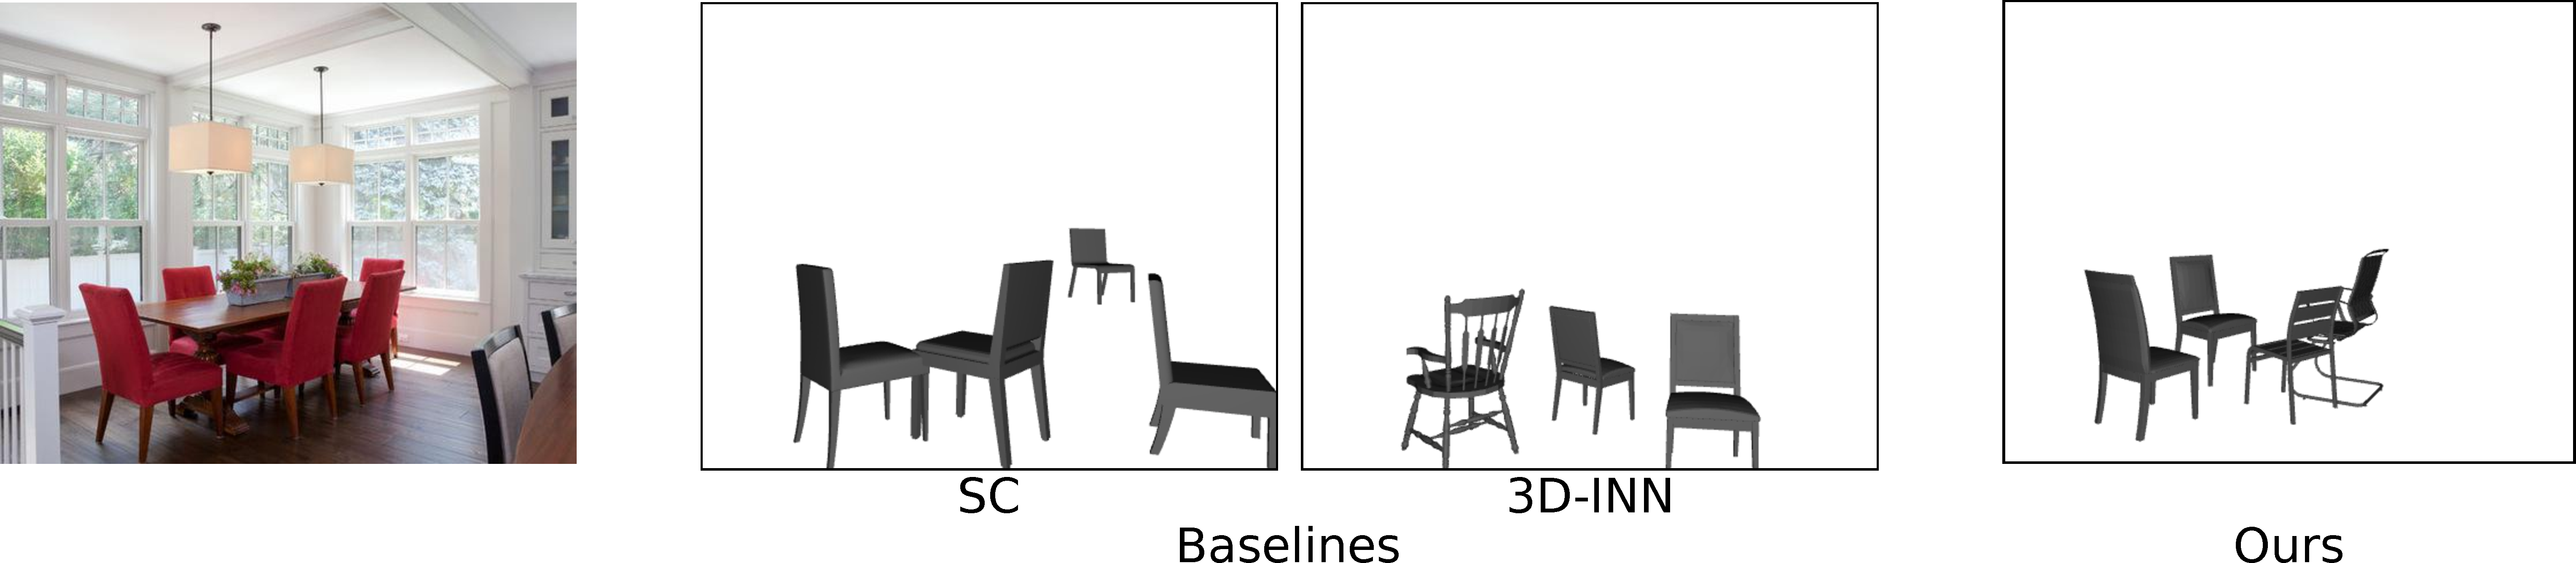
\includegraphics[width=\linewidth]{figures/baseline_foreshadowing/baseline_foreshadowing}
    \caption[Baseline sample]{Methods based only on the image quickly fail in the presence of less than ideally visible chairs. Our method deals with this situation much better.}
    \label{fig:ch4:baseline_foreshadowing}
\end{figure}


To understand this failure, and more importantly how to circumvent it, it is
useful to consider how we as humans are capable of understanding these kind of
scenes. Looking at Figure~\ref{fig:ch4:context_example}, we see a selection of chairs, some
heavily occluded and some clearly visible, in different conditions: (i)~we see the full scene, (ii)~only the local context, or (iii)~only  the pixels that belong to the chair
itself. Observe that the
environment is not important for the recognition of the unoccluded chair  -- the shape of the object is clearly visible and
we immediately recognize the chair. However, under heavily occlusion, the
task of recognizing the chair becomes easier as more context gets added. For
the last column, we might hypothesize that the image regions belong to a chair,
but we have no way of confirming this for certain -- unless the context is
restored.

\begin{figure}
    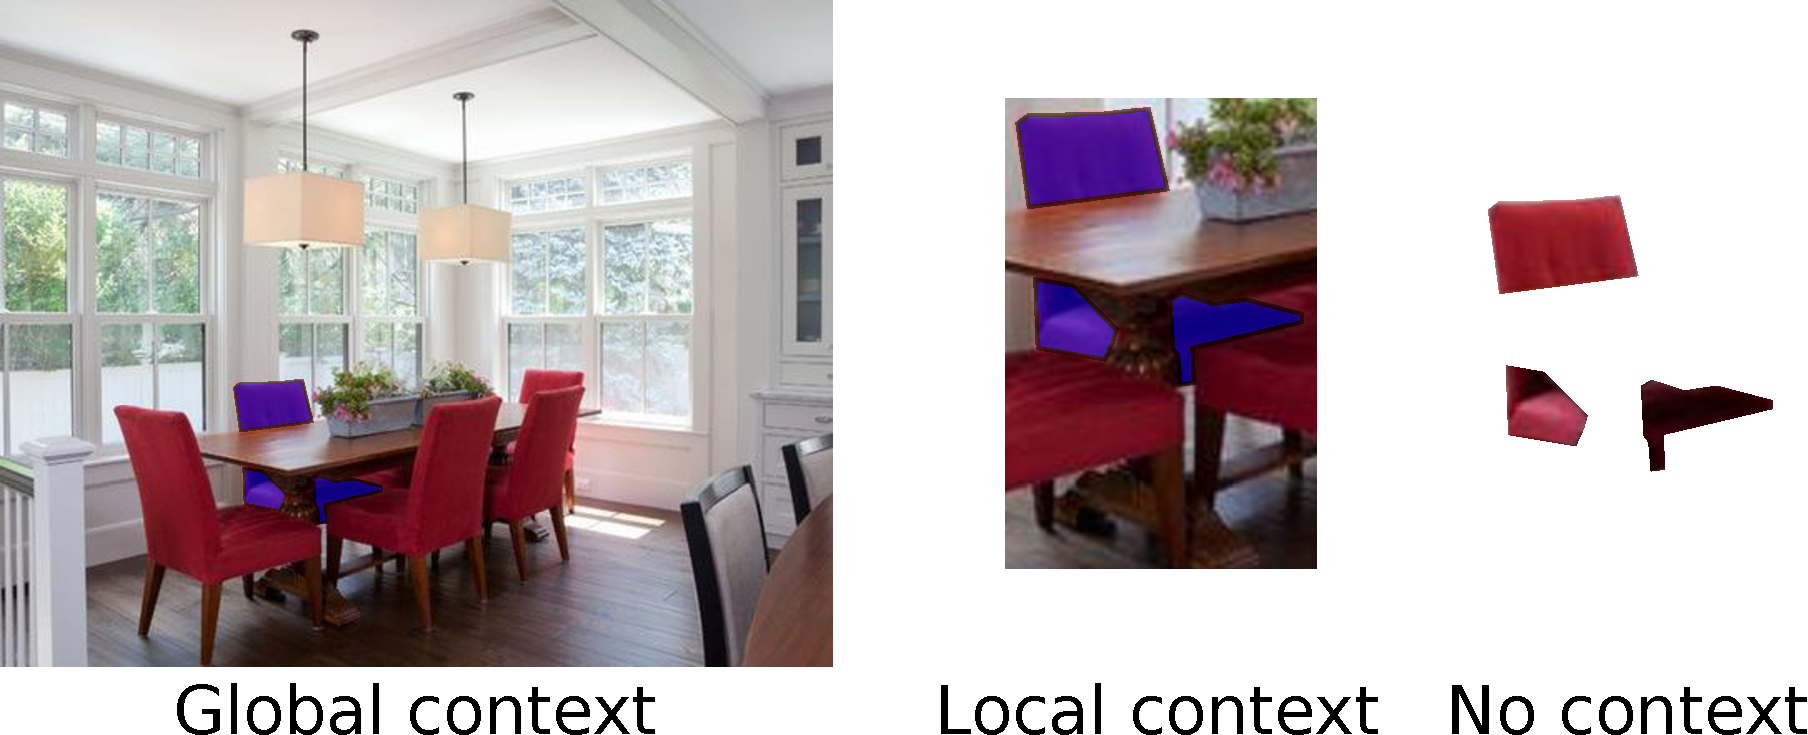
\includegraphics[width=\linewidth]{figures/context_example/context_example}
    \caption[Decreasing context]{As humans, our understanding of scenes is heavily predicated on
    the context. From left to right, less global information is available,
making the classification of the marked object as ``chair'' harder}
    \label{fig:ch4:context_example}
\end{figure}

We observe that the addition of context provides extra information in classifying and
posing the objects in a scene.   Importantly,
the extra information obtained from the entire image is only useful
given prior knowledge we have built up over previous experiences.  In this
particular example, the added context helps only because we know that chairs
often occur together with other chairs and tables.  Given this prior knowledge
and the global context of the object, our recognition efficacy is enhanced.

This insight is what we capture in our approach to the scene mockup problem: to
maximize performance on the mockup task, we need to consider both local
information and the context the objects are placed in. Furthermore, to
understand this context we need to teach the system what usual scenes look like.

We express these notions in our method as follows: we  extract \emph{local}
information from the input image using a keypoint detection network
(Section~\ref{sec:ch4:keypoint_maps}), then \emph{model} the prior knowledge
about how scenes are usually arranged (Section~\ref{ssec:ch4:scene_statistics}),
finally combining this model with the keypoints to find chair instances from a
\emph{global} perspective (Section~\ref{ssec:ch4:graph_optimization}).  The
added high level information pushes the performance past that of the
alternative approach of using only the input data itself (see
Figure~\ref{fig:ch4:baseline_foreshadowing}, right).  In the next section, we
will go through each of these steps in detail.

%-------------------------------------------------------------------------
\section{Method}
\begin{figure}[h!tb]
    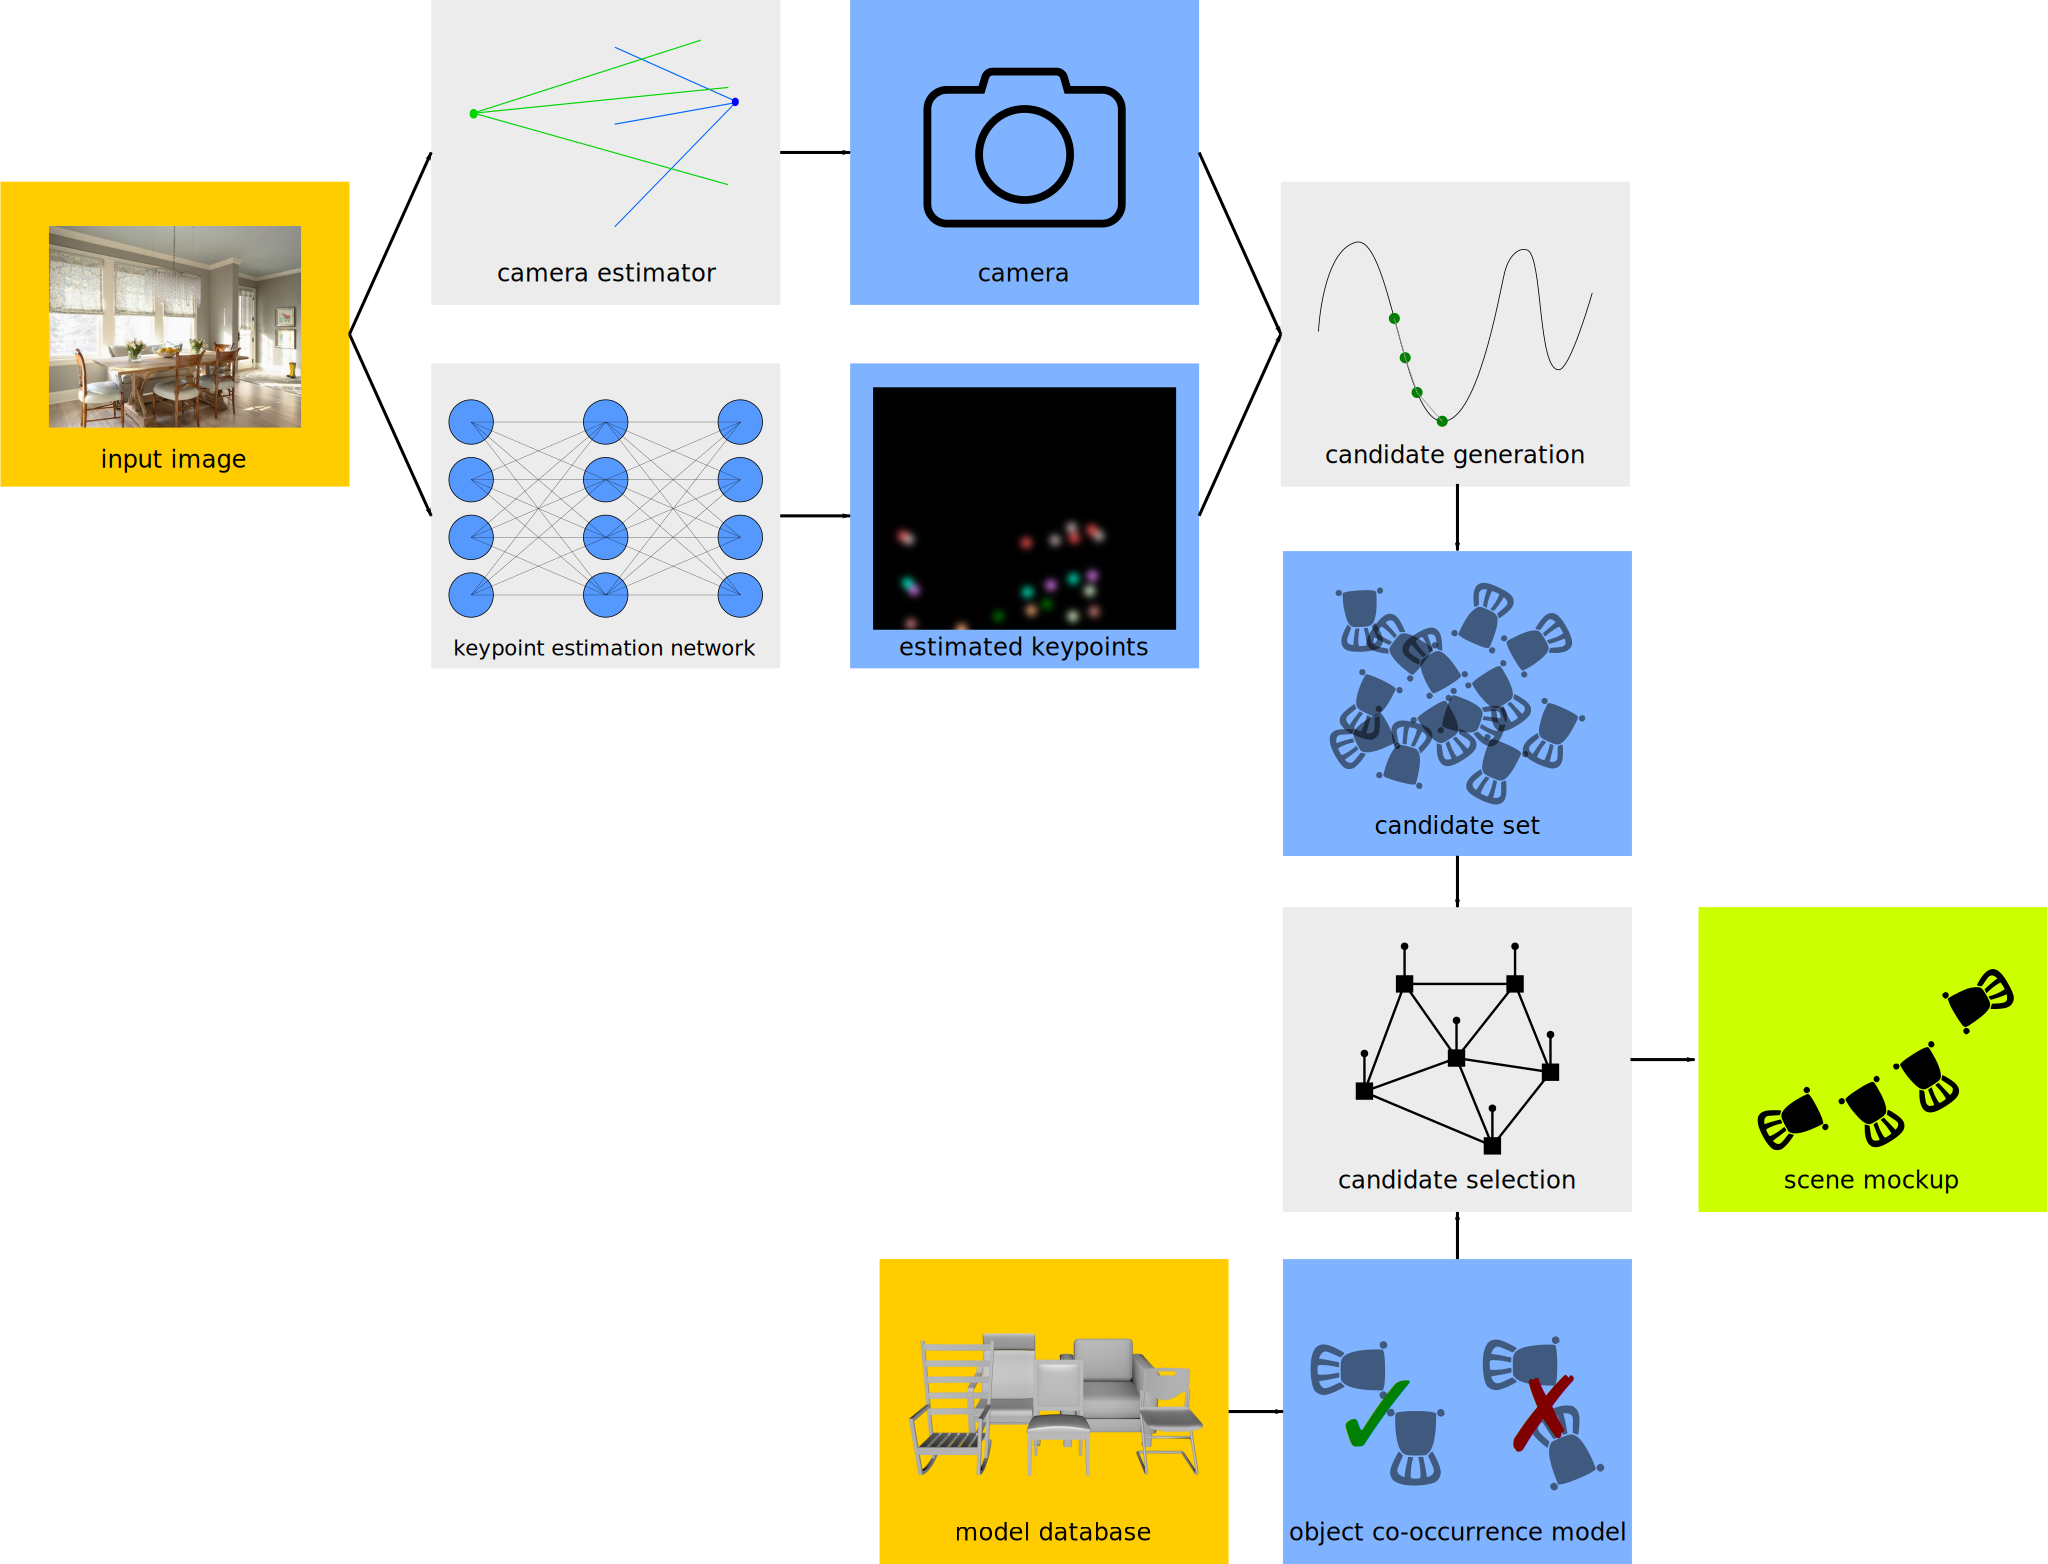
\includegraphics[width=\linewidth]{figures/pipeline/pipeline}
    \caption[Pipeline]{The full pipeline of our method.}
    \label{fig:ch4:pipeline}
\end{figure}
Our pipeline (Figure~\ref{fig:ch4:pipeline}) takes as input a photograph $\bb{x}$ and a database of 3D chair models
$\bb{M}$, and outputs a mocked up 3D scene $\bb{S}$, such that the reprojection
of $\bb{S}$ with the  estimated camera $C$ results in an image that approximates the photograph  $\bb{x}$ (see Figure~\ref{fig:ch4:intended_outcome}).
%The scene consists of chairs $o_i \in S$, where $o_i = \{t_i, \theta_i, s_i\}$
%and $t_i$ is the chair's translation, $\theta_i$ is the chair's rotation around
%the up-axis and $s_i$ is the chair's scale. 

\begin{figure}[t]
    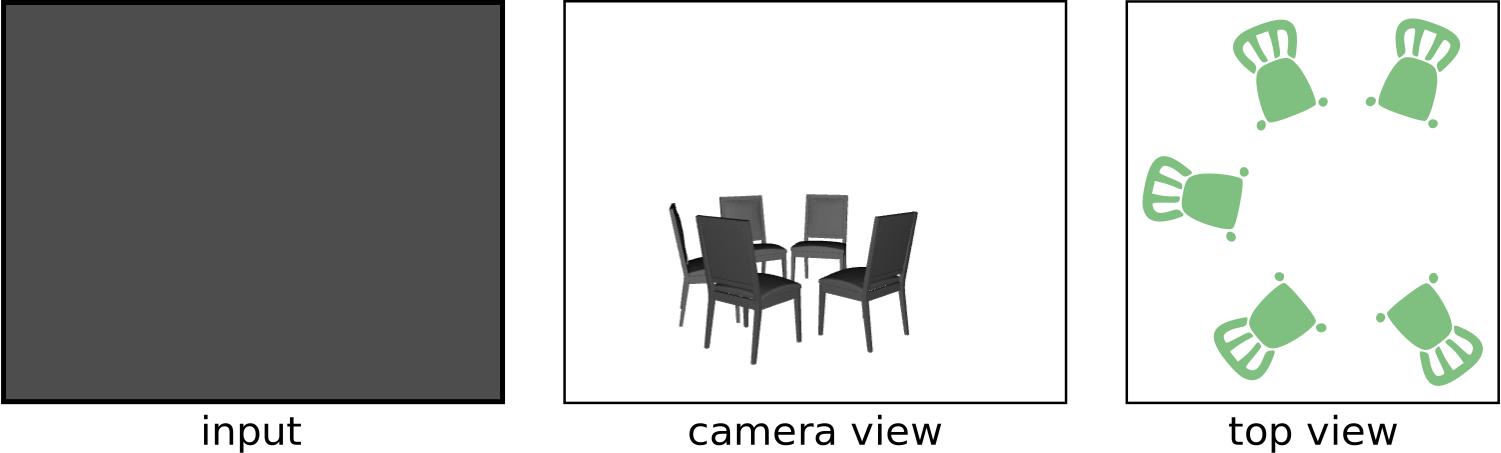
\includegraphics[width=\linewidth]{figures/expected_output/expected_output}
    \caption[Expected output]{Intended working of our method: we take a single image of a structured indoor scene as input, and output a 3D scene with the constituent chairs recovered in the right location and pose, as well as the camera parameters that reproject this scene as close as possible to the original input.}
    \label{fig:ch4:intended_outcome}
\end{figure}

As preprocessing, we estimate the scene camera $C$  using an
vanishing directions~\cite{Hedau:2009:ICCV} to obtain focal length and
camera orientation (Section~\ref{sec:ch4:camera_estimation}). Our method consists of  three stages: (i)~the image is
passed through a keypoint estimation network that outputs a set of
\emph{keypoint probability maps}, representing at each pixel the probability of
the presence of a certain semantically meaningful keypoint
(Section~\ref{sec:ch4:keypoint_maps}); 
%
(ii)~the keypoint maps
are combined with the estimated camera $C$ to generate candidate object
placements (Section~\ref{sec:ch4:candidate_generation}); and  
%
(iii)~a
selection is made among these candidates by optimizing an objective function
which combines object-to-keypoint-map matching with pairwise placement agreement
according to a pre-trained object co-occurrence model
(Section~\ref{sec:ch4:optimization}). The second and third stages are then
iterated, this time taking into account the previously found objects during
candidate generation as a strong prior (Section~\ref{sec:ch4:iteration}). This
process is iterated until convergence. 


\subsection{Camera estimation}
\label{sec:ch4:camera_estimation}
To convert sets of 2D keypoints to possible 3D locations we need the intrinsic
and extrinsic parameters of the camera with which photo $\bb{x}$ was taken.
Specifically, for a good reconstruction, we need the orientation of the camera
with respect to the ground plane in the form of rotation matrix $C_R$, the
focal length $C_f$, and a measure of the scale of the room $C_s$.  However,
estimating the scale of the room without prior information is not possible -- even
if we know the 2D location of a chair, it still might be 1 meter or 100 meters tall. There is no way of deciding this
without some prior knowledge about chairs and their dimensions. We thus fix our
scale parameter and only estimate $C_f$ and $C_R$, and replace $C_s$ with
individual scale parameters for each object in the optimization later on.  Most
methods for camera parameter estimation indeed focus on $C_f$ and $C_r$, and to
do so rely on automatically estimating vanishing points (see
Figure~\ref{fig:ch4:camera_estimation}). We employ the method from Hedau et
al.~\cite{Hedau:2009:ICCV}. In summary, their method uses structured learning
from Tsochantaridis et al.~\cite{Tsochantaridis:2005:JMLR} to rank multiple
room layout candidates, which are generated from estimated vanishing points. We
refer to the paper from Hedau et al. for more information.

To complete our camera parameters, we pick meters as unit in our world
coordinate system (the same coordinate system used by our model set), and set
the camera's location $C_t$ as being at eye height (1.8m) on world origin. This
altogether yields our camera $C$.

\begin{figure}
    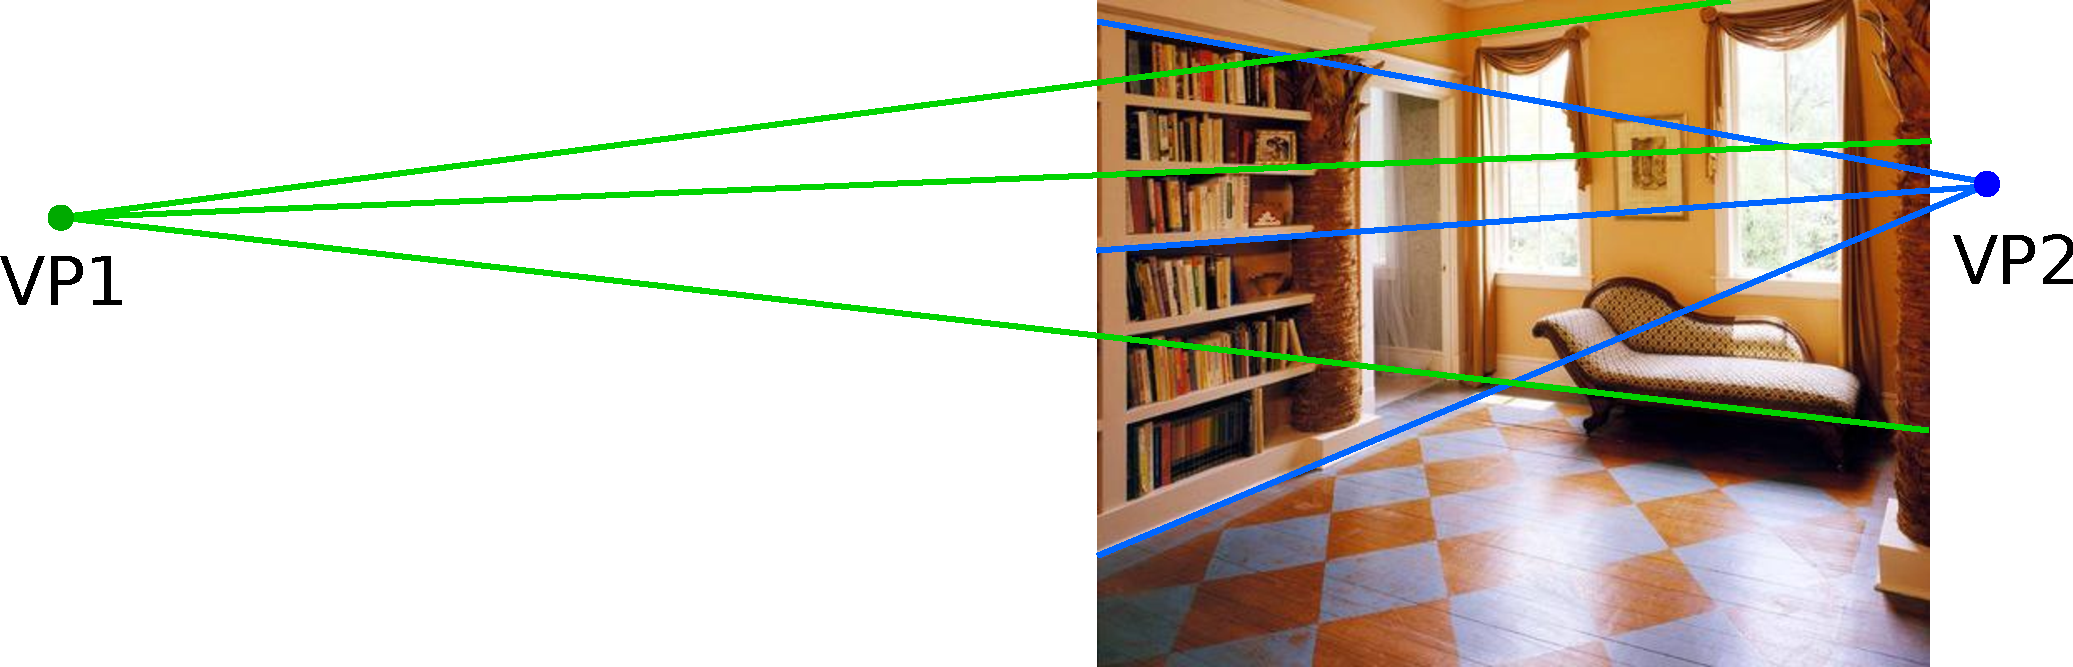
\includegraphics[width=\linewidth]{figures/camera_estimation/camera_estimation}
    \caption[Vanishing point detection]{By estimating vanishing points in the image, the camera rotation matrix and focal length can be detected. Detecting scale a priori is not possible.}
    \label{fig:ch4:camera_estimation}
\end{figure}

\subsection{Keypoint maps}
\label{sec:ch4:keypoint_maps}
Our goal is to find location and pose of as many chairs in the scene as possible.
We aim to do this by finding all instances of a predefined set of
semantically meaningful keypoints in the image, and then use the estimated camera together with a
3D chair template consisting of those same keypoints to reconstruct
the 3D location and pose of the chairs.

We start by defining a set of general keypoint types for the chair object class.
Each keypoint type represents one or more keypoints that should be present in
each (reasonable) chair instance. We selected 8 keypoint types, each of which
is uniquely identifiable on every reasonable chair. These keypoint types
are shown in Figure~\ref{fig:ch4:keypoint_types}.

%\paragraph{Note on object symmetry} Ideal are unique keypoint types, i.e.
%types that occur only once on each instance of the object class.  Because of
%certain symmetries, for certain classes of object this is not always possible.  In
%Figure~\ref{fig:ch4:keypoints} the keypoints for the ``chair'' and ``table''
%class are shown. Note that for chairs, the keypoints are all unique.  In
%contrast, the top corners of the ``table'' class cannot be unambigously
%distinguished from eachother under shape variation and rotation around the
%up-axis.
\begin{figure}[h!tb]
    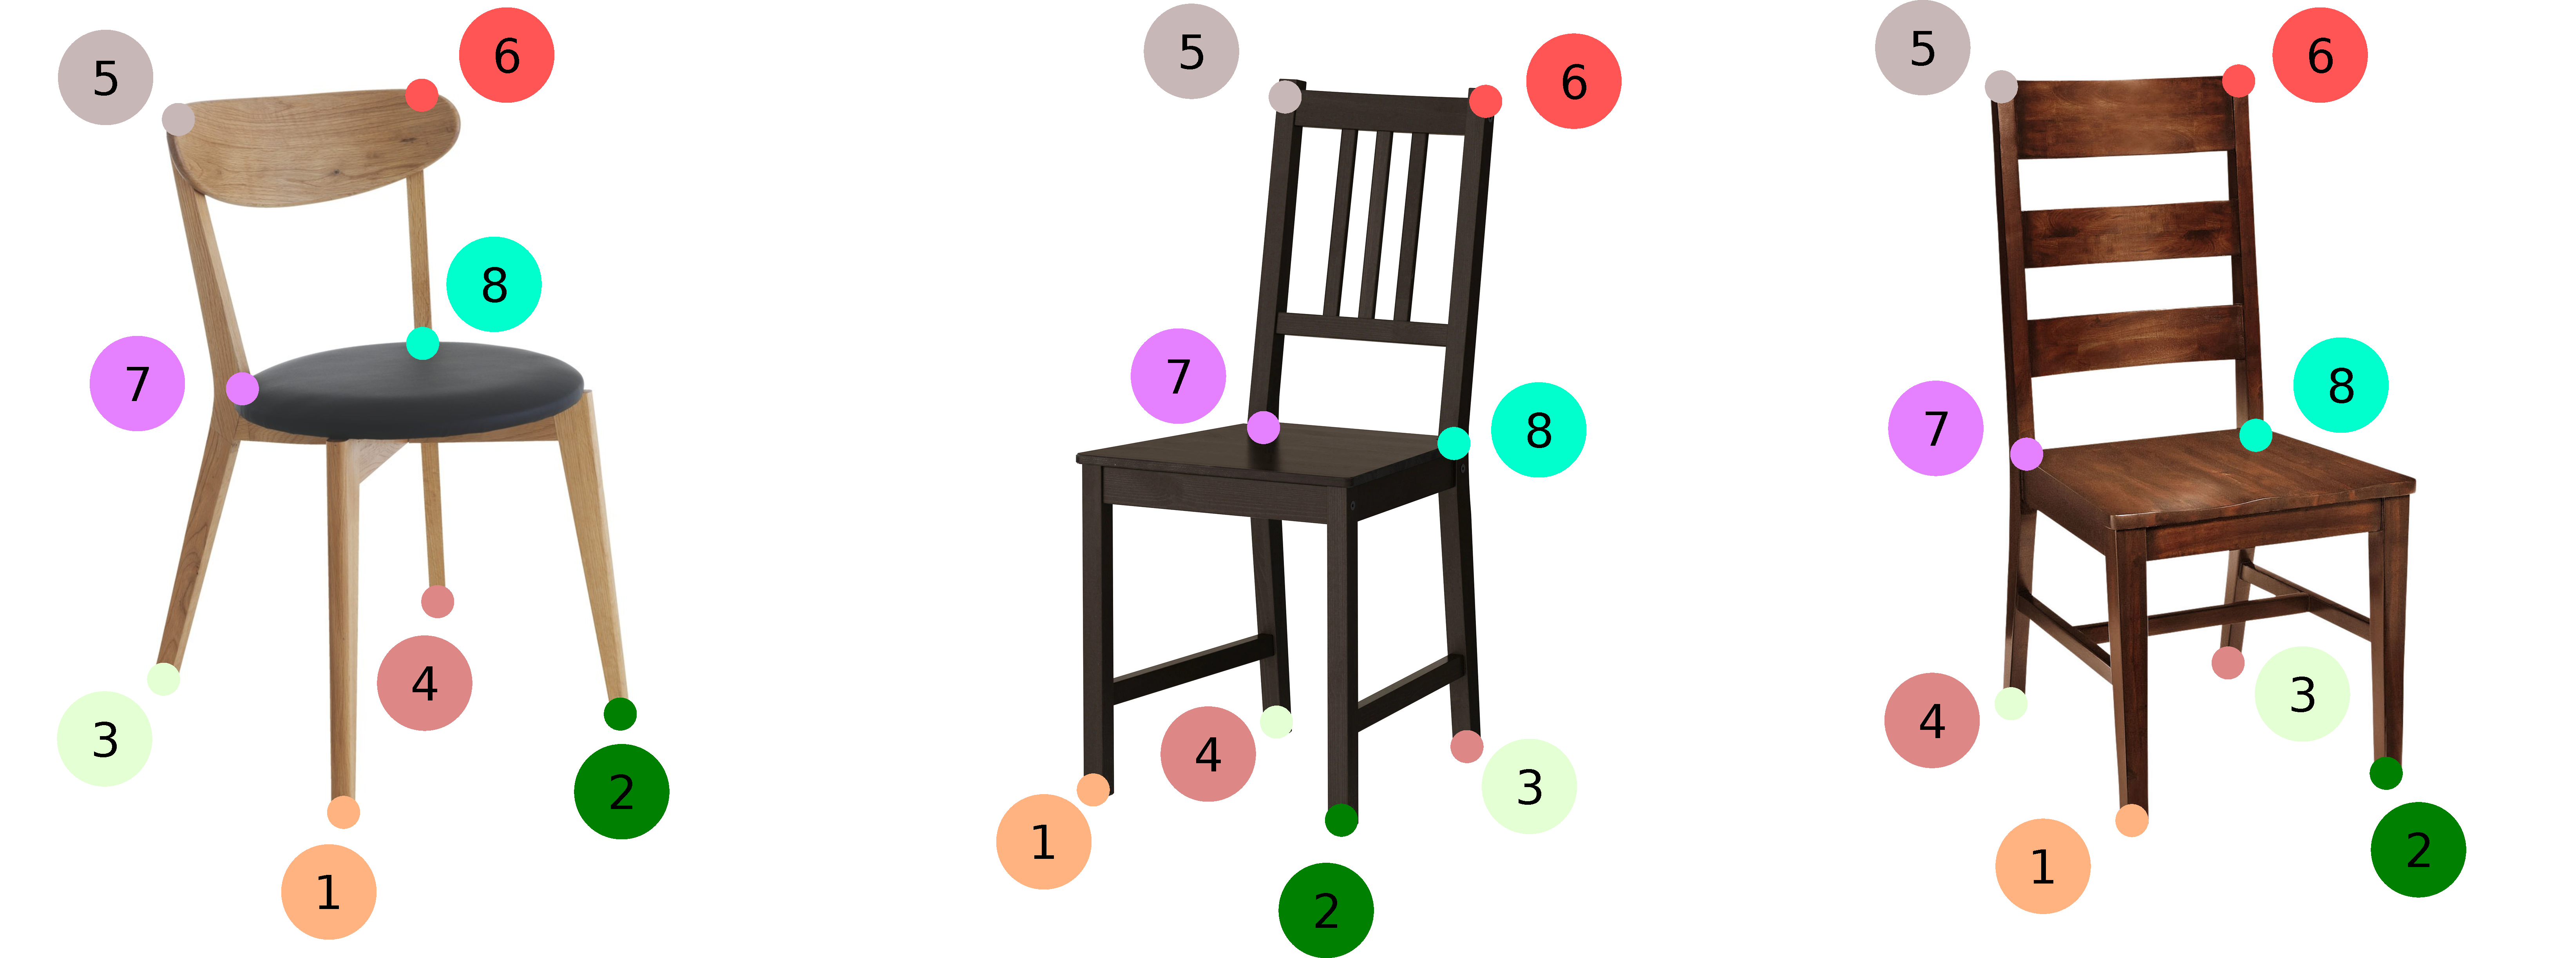
\includegraphics[width=\linewidth]{figures/keypoint_types/keypoint_types}
    \caption[Keypoint types]{Selected keypoint types.}
    \label{fig:ch4:keypoint_types}
\end{figure}

%We stress that the 2D locations of the detected keypoints will be used in
%combination with the found camera parameters $C$ to optimize for the placement
%of a parameterized 3D object template with those same keypoints.  Were the
%object template fixed, knowing 3 correspondences between 3D and 2D keypoints
%would fully define the 3D similarity transform of the template. As we will also
%add the constraint of rotation only being allowed around up-axis, a
%fully-constrained system is achieved with just 2 correspondences.  However, as
%our template is not fixed (i.e. the parameters of the PCA-based template are
%also solved for), 
%
%For a fixed 3D mesh, knowing 3 correspondences between 

\subsubsection{Keypoint location map}
A keypoint location map is a 2D map whose domain is the input image $\bb{x}$, and
represents belief about the presence of a specific keypoint type at a specific
pixel of $\bb{x}$. It is represented as a $r \times r$ single-channel
matrix, with values between 0 and 1. In the case of perfect information, the matrix will have
value 0 everywhere except for those locations where a keypoint of the
corresponding type is present, where it would have value 1. However, as we will employ
an L2 loss function, such step-function keypoint maps would result in an extremely
discontinuous error landscape, destabilizing the training process.  Instead, we
represent each keypoint using a Gaussian lobe centered around its true location,
 resulting in a much smoother loss function (see Figure~\ref{fig:ch4:keypoint_lobes}).

\begin{figure}
    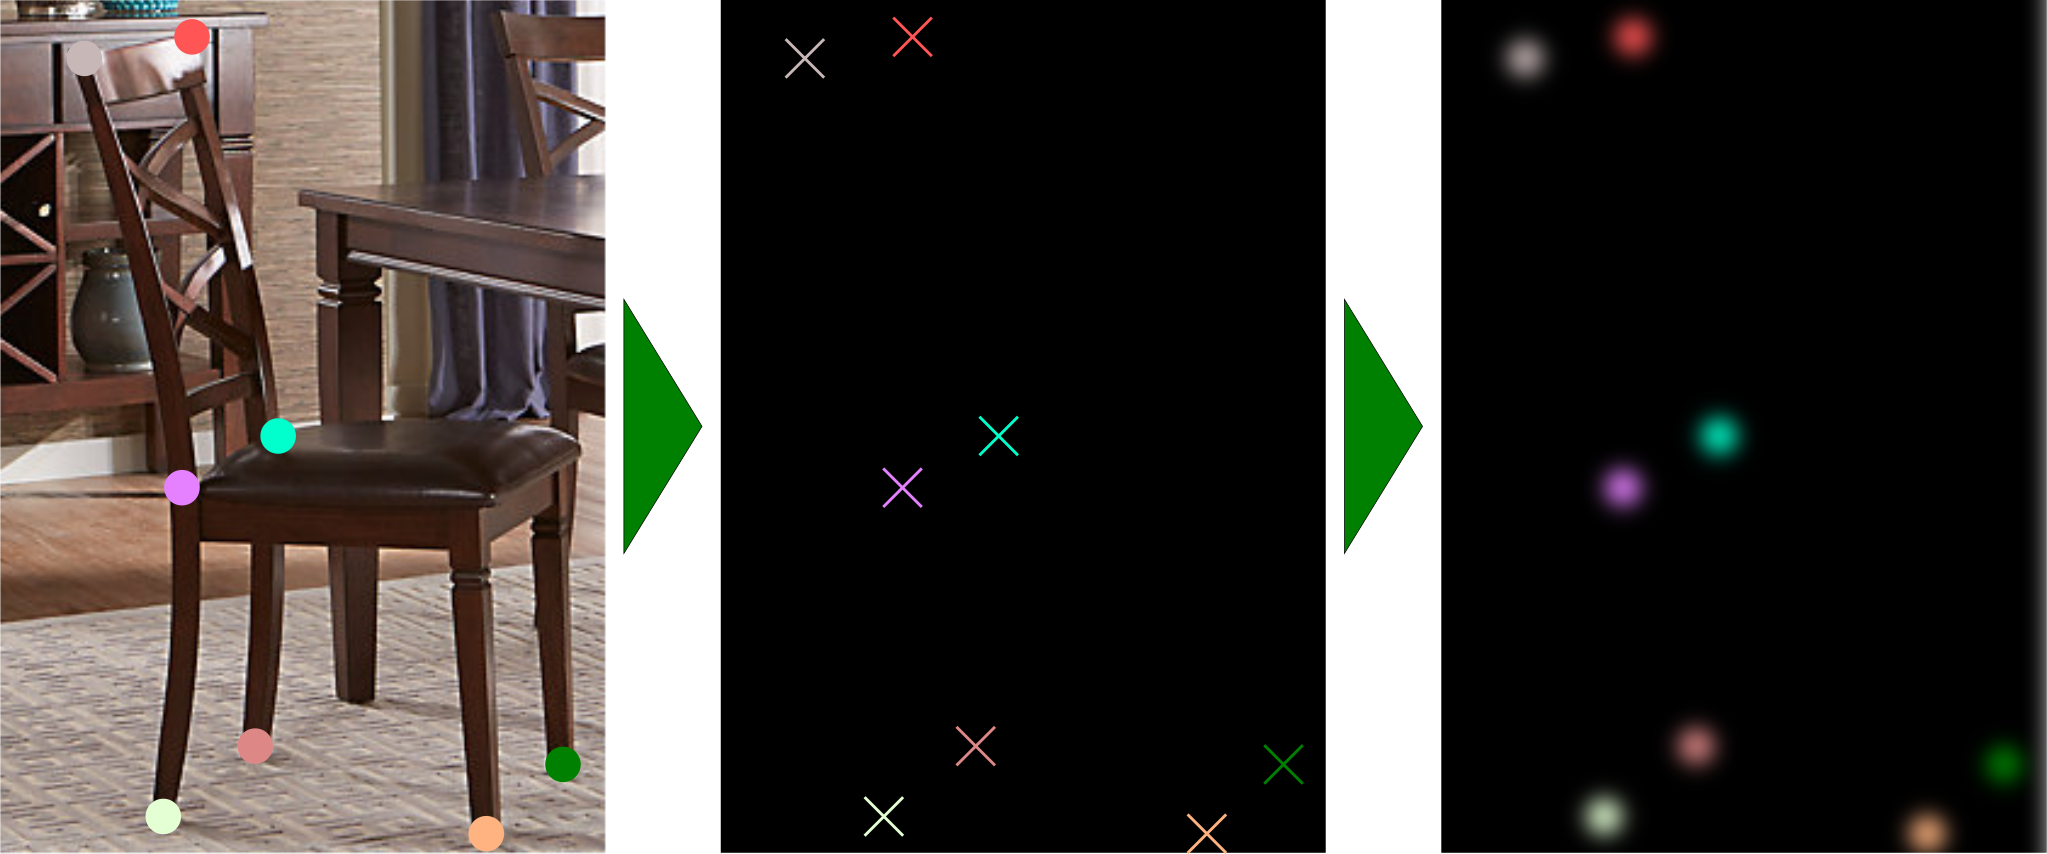
\includegraphics[width=\linewidth]{figures/gaussian_lobes/gaussian_lobes}
    \caption[Gaussian lobes]{To facilitate the training process the keypoints are represented as Gaussian lobes around their location.}
    \label{fig:ch4:keypoint_lobes}
\end{figure}

\subsubsection{Keypoint estimation network}
To extract keypoint location maps for each keypoint type from an input image,
we employ a deep learning architecture.  This network takes our image $\bb{x}$ as
input and outputs a set of keypoint location maps $m_1, \ldots, m_{N_k}$, where
$N_k = 6$ is the total number of predefined semantic keypoints.

The network architecture was selected through experimentation. We tried 2 different architectures:
\begin{itemize}
    \item The convolutional pose machines (CPM) \cite{Wei:2016:CVPR} architecture,
          whose task of human pose estimation through keypoint localization closely resembles our own, and
    \item ResNet-50 \cite{He:2016:CVPR}, a general purpose network with high
          performance on a number of image understanding tasks, such as object detection and semantic segmentation.
\end{itemize}
In both cases, we trained the network using an L2 loss function on the difference between
the output and ground truth keypoint location maps.

Perhaps surprisingly, ResNet-50 resulted in the highest test accuracy (see
Table~\ref{tab:ch4:net_performance}).  Although the task that CPM was meant for
(keypoint detection) more closely resembles our own, it cannot compete with the
fact that ResNet-50 was pretrained on ImageNet, the data distribution of which
is more similar to ours.

\begin{table}
    \centering
    \begin{tabular}{|c|c|}
        \hline
        architecture & MSE \\ \hline
        ResNet-50~\cite{He:2016:CVPR} & $3.24 \times 10^{-5}$ \\ \hline
        CPM~\cite{Wei:2016:CVPR} & $1.02 \times 10^{-4}$ \\ \hline
    \end{tabular}
    \caption[Architecture performance]{Performance of the two tried architectures on our task. ResNet-50's advantage of being pretrained on ImageNet gives it the edge over CPM.}
    \label{tab:ch4:net_performance}
\end{table}

We employed the TensorFlow implementation of ResNet-50. By using an input image
size of $512 \times 512$ and a bottleneck stride of 8 we get a final keypoint
map size of $r = 64$. The full architecture can be seen in Table~\ref{tab:ch4:network_architecture}.
The training data we used is discussed in Section~\ref{sec:ch4:training_data}.

\begin{table}[h!tb]
    \centering
    \resizebox{\linewidth}{!}{
        \bgroup
        \def\arraystretch{1.5}
        \begin{tabular}{|c|c|c|}
            \hline
            layer name & output size & node type \\ \hline
            input      & $512 \times 512$ & \\ \hline
            conv\_1     & $256 \times 256$ & $7\times 7$, stride 2 \\ \hline
            max\_pool   & $128 \times 128$ & Max pooling, stride 2 \\ \hline
            block\_1 & $64 \times 64$ & Bottleneck units with shortcuts, $\begin{bmatrix} 1 \times 1, 64 \\ 3 \times 3, 64 \\ 1 \times 1, 256 \end{bmatrix} \times 3$, last $3\times 3$ stride 2 \MatTableStrut \\ \hline
            block\_2 & $64 \times 64$ & Bottleneck units with shortcuts, $\begin{bmatrix} 1 \times 1, 128 \\ 3 \times 3, 128 \\ 1 \times 1, 512 \end{bmatrix} \times 4$, all stride 1 \MatTableStrut \\ \hline
            block\_3 & $64 \times 64$ & Bottleneck units with shortcuts, $\begin{bmatrix} 1 \times 1, 256 \\ 3 \times 3, 256 \\ 1 \times 1, 1024 \end{bmatrix} \times 6$, all stride 1 \MatTableStrut \\ \hline
            block\_4 & $64 \times 64$ & Bottleneck units with shortcuts, $\begin{bmatrix} 1 \times 1, 512 \\ 3 \times 3, 512 \\ 1 \times 1, 2048 \end{bmatrix} \times 3$, all stride 1 \MatTableStrut \\ \hline
        \end{tabular}
        \egroup
    }
    \caption[Network architecture]{ResNet-50 based architecture used for keypoint estimation.}
    \label{tab:ch4:network_architecture}
\end{table}

\subsection{Candidate generation}
\label{sec:ch4:candidate_generation}
Now that the camera parameters and keypoint locations have been estimated, we
move on to the candidate generation stage. In this part, predefined object templates
are fit to different subsets of the estimated keypoint locations, and scored
by their agreement with the entire keypoint map. First, we will describe how we get specific
keypoint locations from the estimated keypoint maps. Then, we will discuss how we construct
the object templates from our set of 3D models. Finally, we describe the actual
candidate generation process.

\subsubsection{Keypoint locations from keypoint location maps}
The keypoint estimation network's output consists of $N_k$ single channel
keypoint location maps $m_1, \ldots, m_{N_k}$. For our candidate generation process, these maps need
to be converted to concrete keypoint locations. We cannot simply take all
locations with a value above a certain threshold, as the maps spread the
probability of a found keypoint across multiple pixels (Figure~\ref{fig:ch4:keypoint_lobes}).  One way of dealing
with this is to find all local maxima in each map. The issue with this is that
large regions of very low probability still have many local maxima. To discount
these, we first pass each map $m_i$ through a thresholding operation with
threshold $\tau_m$, discarding all pixels below that value.  Then, we find all
8-neighbourhood local maxima in each map $m_i$, and store them as our candidate keypoint
locations. We denote the found keypoint locations of type $k$ as $\bb{Q}_k$, and the
full set $\bb{Q} = \{\bb{Q}_1, \ldots, \bb{Q}_{N_k}\}$.  See
Figure~\ref{fig:ch4:keypoint_map_to_keypoints}.

\begin{figure}[h!tb]
    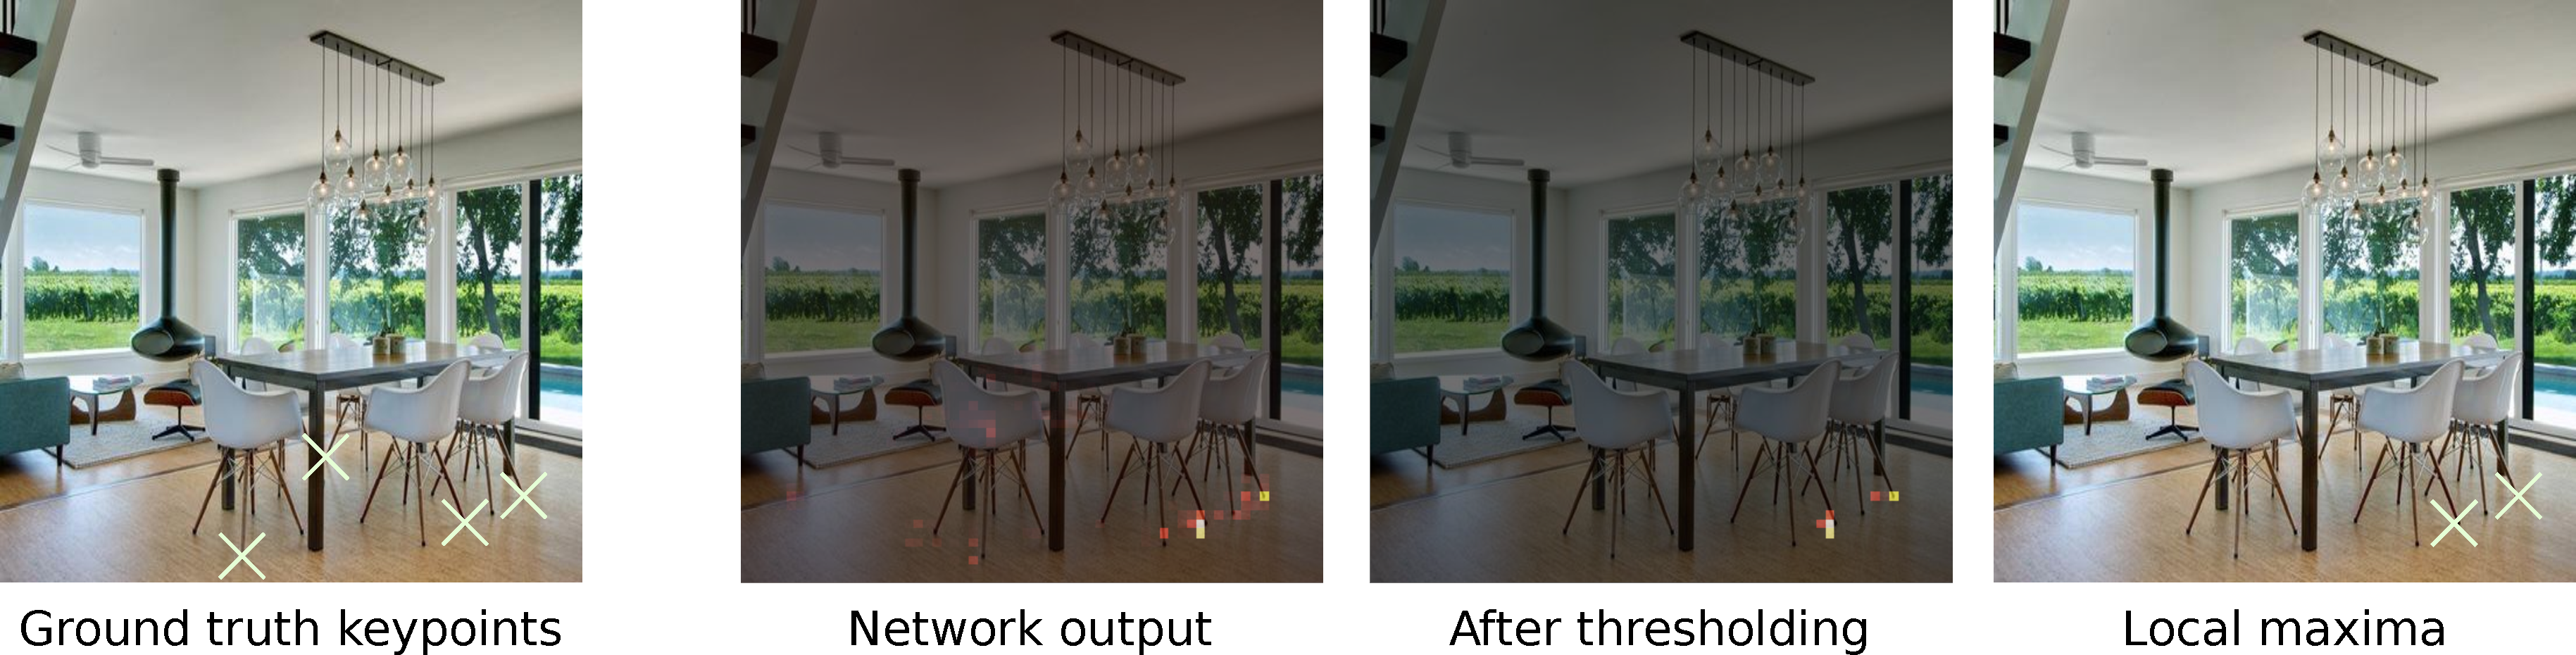
\includegraphics[width=\linewidth]{figures/keypoint_map_to_keypoints/keypoint_map_to_keypoints}
    \caption[Keypoint map postprocessing]{Keypoint candidate locations are found by thresholding the output of the neural network and then finding local maxima}
    \label{fig:ch4:keypoint_map_to_keypoints}
\end{figure}


%We now have a set of candidate keypoints for each of the $N_k$ keypoint types.
%Given a subset of distinct keypoints we can use the estimated camera to fit an annotated chair model to this set
%
%Together with the estimated camera, we can fit any 3D chair model which has been annotated with these same keypoints
%to these 2D keypoints. 
%
\subsubsection{Object templates}
From the keypoint candidates $\bb{Q}$, we want to find actual chair
candidates. As all chairs are slightly different in shape, and fitting each
chair model in our dataset individually is prohibitively expensive, we make use
of a chair template model.

Specifically, we create this chair template model by fitting a Principal
Component Analysis (PCA) basis to the 3D coordinates of all 8 keypoints of all
chair models in our database $\bb{M}$.  By analysing the cumulative
percentage of variance of each resulting PCA dimension, we conclude that the
top 3 PCA dimensions are responsible for $>85\%$ of variance in the shape of
all chairs. These top 3 PCA dimensions represent our chair template model $T$, and
the deviation from the mean $\bb{p} \in \mathbb{R}^3$ represents a variable for our optimization.
See Figure~\ref{fig:ch4:pca_dimensions}.

\begin{figure}[h!tb]
    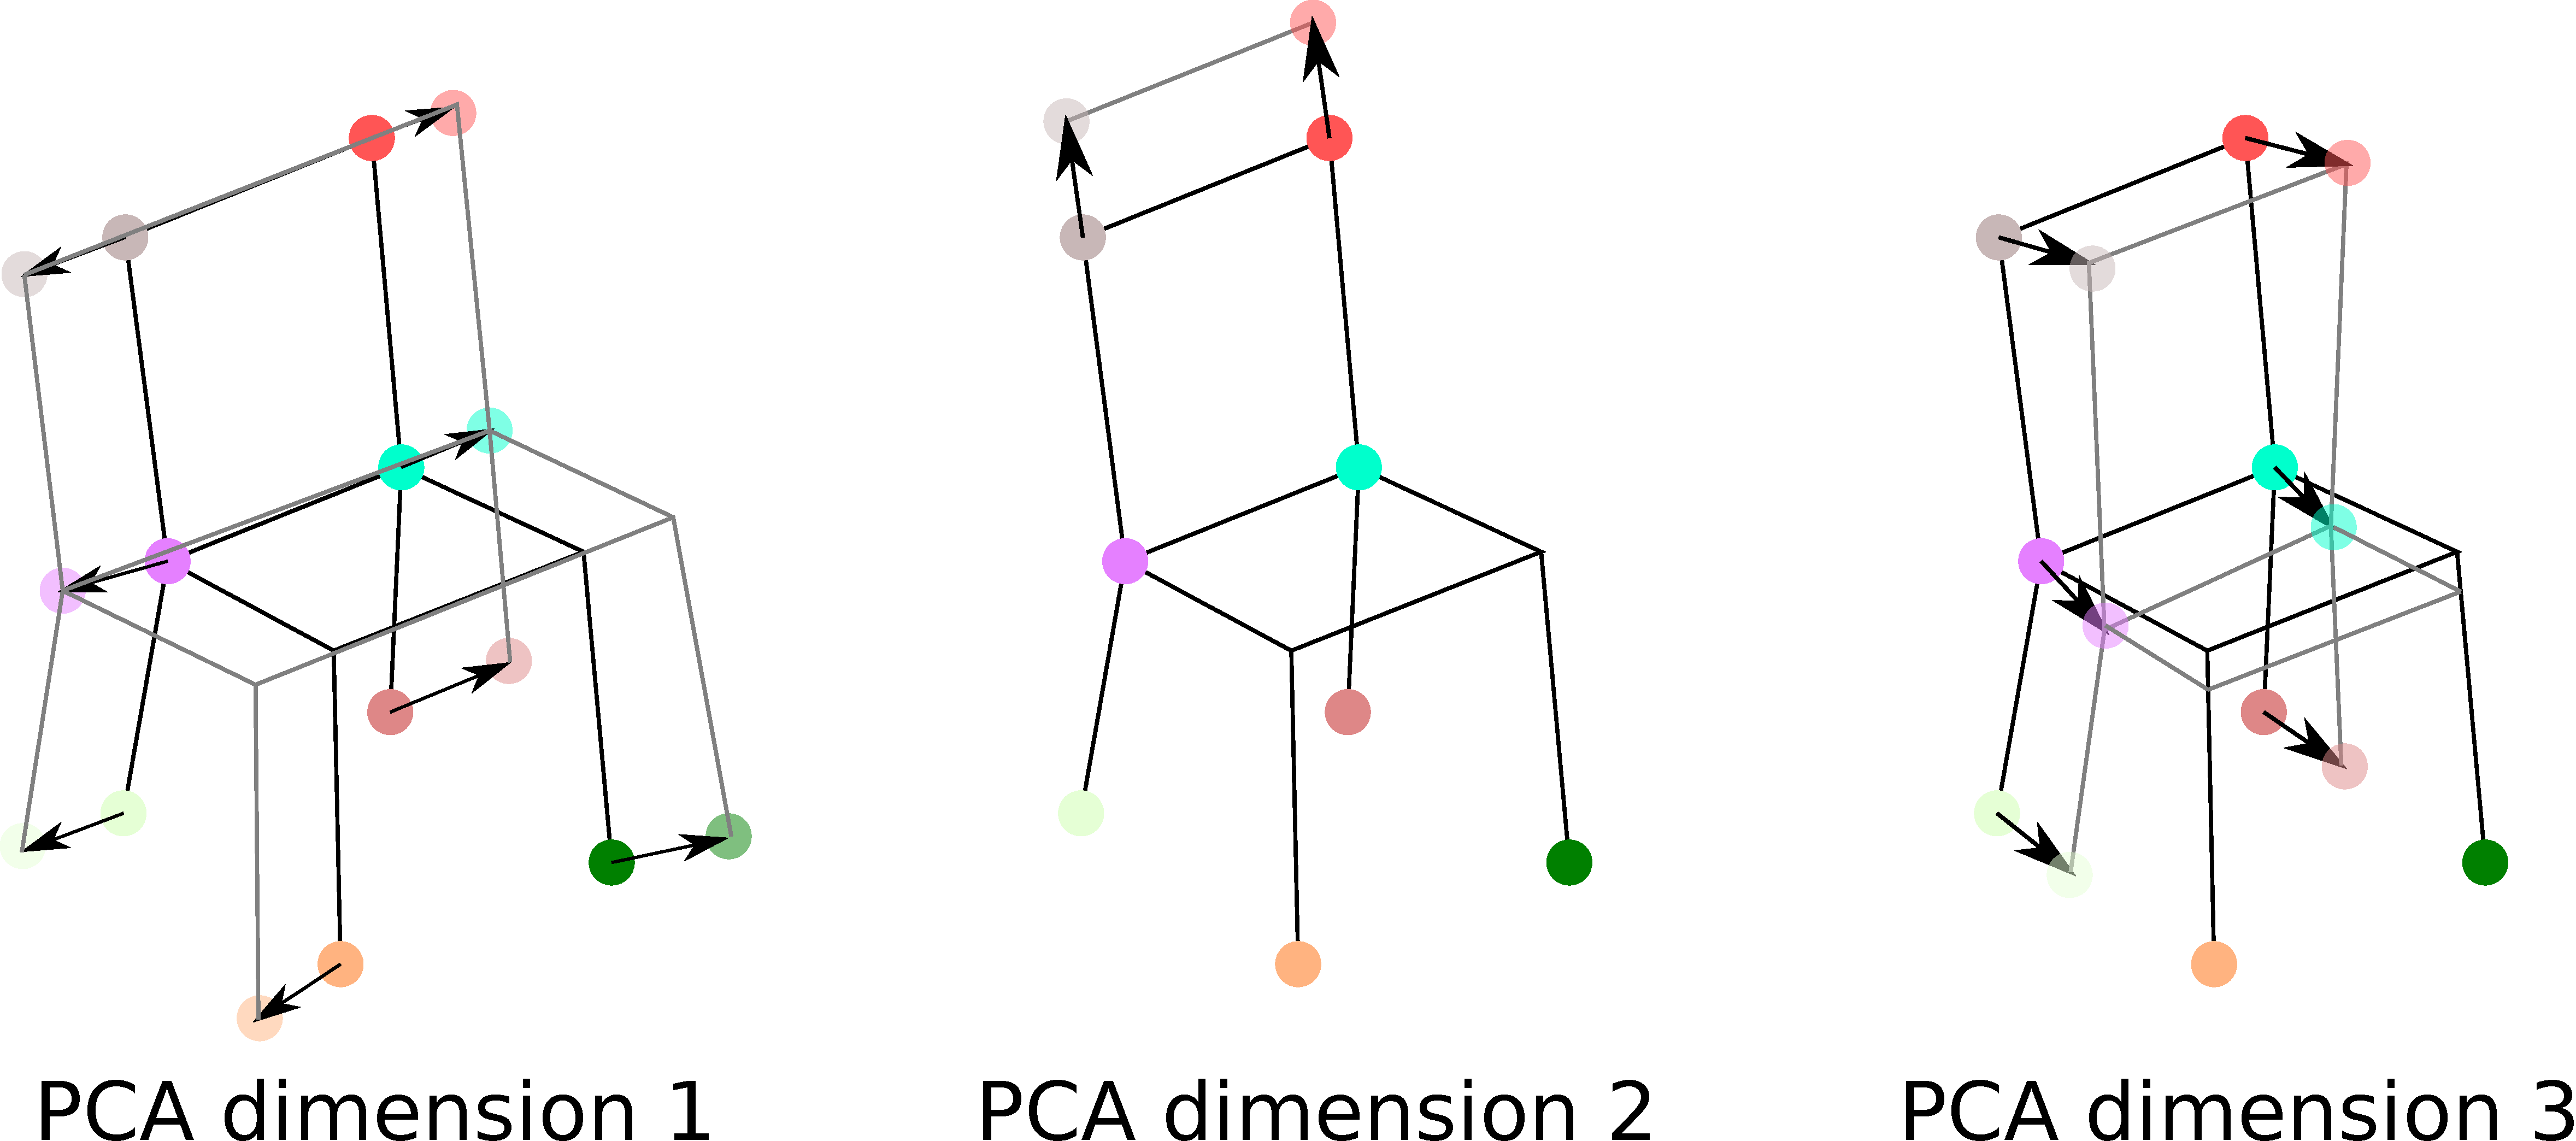
\includegraphics[width=\linewidth]{figures/pca_dimensions/pca_dimensions}
    \caption[Template PCA]{Visualization of the top 3 PCA dimensions of our chair template, with respect to the mean chair. They approximately correspond to respectively chair width, back height and chair depth.}
    \label{fig:ch4:pca_dimensions}
\end{figure}

We define $T(\bb{p})$ as the reprojection of PCA parameters $\bb{p}$ to 3D world space, i.e.
the instantiated coordinates of one particular instance of the chair template.

\vspace{-1mm}
\subsubsection{Candidate keypoint sets}
Finally, we will fit the generated chair template $T$ to the found keypoint
locations $\bb{Q}$.  Unfortunately, we do not have any correspondences between the
keypoint locations of different types -- for example, we do not know which
``top-left'' keypoint belongs with which ``front-right-leg'' keypoint.  As
such, we generate the exhaustive set of candidates by fitting a candidate chair
placement to each minimum set of 2D keypoint locations that results in a
well-defined fitting problem. A single keypoint correspondence is not enough,
as any candidate placement can then be rotated around its up-axis
indiscriminately. As we know the camera and thus the ground plane, and work
under the assumption that the chair models can change only scale and azimuth
(i.e. are placed flat on the ground), we can suffice with 2 keypoint
correspondences. Although this does leave some ambiguities due to overlap
between the scale dimension and the template parameters, due to regularization
on both of these parameter sets the resulting problem is well-defined. We thus
create our set of 2D keypoint candidate pairs as

\[ \bb{K} = \bigcup_{\bb{Q}_i \in \bb{Q}}\bigcup_{\bb{Q}_j \in \bb{Q}\setminus{}\bb{Q}_i} \bb{Q}_i \times \bb{Q}_j, \]

where $\times$ represents the Cartesian product.

\subsubsection{Template fitting}
\label{sssec:ch4:template_fitting}
\begin{figure}[h!t]
    \def\svgwidth{\linewidth}
    \import{figures/notation/}{notation.pdf_tex}
    \caption{Parameters estimated during the candidate fitting process.}
    \label{fig:ch4:fitting_parameters}
\end{figure}
Then, we will generate one candidate chair placement for each $\bb{K}_i \in \bb{K}$
by finding the optimal parameters that yield a reprojection of the template's keypoints in line with $\bb{K}_i$,
as well as the full keypoint location maps $\bb{m}$.
These parameters consist of:
\begin{itemize}
    \item a 2D translation across the ground plane $\bb{t}$,
    \item 1D azimuth $\theta$,
    \item 1D scale $s$,
    \item 3D chair template parameters $\bb{p}$.
\end{itemize}
See Figure~\ref{fig:ch4:fitting_parameters} for clarification.  This
optimization is split into two stages.  In the first stage, we will optimize
specifically for the reprojection of the 3D keypoints corresponding to $k_u,
k_v \in \bb{K}_i$.  In the second stage, we will incorporate our knowledge of
the other keypoint location maps in $\bb{m}$ and further finetune the
parameters to match with them as closely as possible as well.  We now describe
each stage in turn.

\paragraph{First stage -- optimization w.r.t. 2 keypoints}
In the first stage, we find the optimal parameters such that the reprojection of the chair template's keypoints line up with $\bb{K}_i$.
We define the reprojection $z_i$ of each keypoint $k_i, i \in \{u, v\}$ as
%
\[ z_i = P(R(s[T(\bb{t})]_i, \theta) + \bb{t}, C), \]
%
where $R$ represents rotation, and $P$ represents camera projection.

The objective function is then simply the summed mean squared error of these reprojections w.r.t. the data:

\[ L = \sum_{i \in \{u, v\}} \|z_i - k_i \|^2 \]. 

We initialize the parameters as $\bb{t} = \bb{0}, \theta = 0, s = 1,
\bb{p} = \bb{0}$. Furthermore, we add an L2 regularization term to both
the norm of the template parameters $\bb{p}$ as well as the scale $s$.
This non-linear least squares optimization problem is then solved using Ceres~\cite{Ceres}.

\paragraph{Second stage -- optimization w.r.t. all keypoints}
Now that the parameters have been optimized w.r.t.\ our keypoint pair $\bb{K_i}$, we 
finetune the parameters by also taking into account the other keypoint location maps in $\bb{m}$.
Note that we now go back to using the keypoint location maps themselves instead
of the extracted local maxima -- we do not optimize for exact location anymore, and
allow the final reprojection to deviate from the maxima in each individual keypoint location map.
Instead, we maximize the \emph{total probability} over all keypoint location maps. Our objective function  becomes:
%
\[ L = \sum_{i \in \{1, \ldots, N_k\}} \|1 - m_i(z_i)\|^2, \]
%
where $m_i(z_i)$ represents the value of keypoint location map $m_i$ at reprojected keypoint $z_i$.
The same L2 regularizations as in the first stage apply, and we again solve our problem using Ceres~\cite{Ceres}.

If the final loss of the second stage is lower than a threshold $\tau_u$ we add the final parameters
as a candidate placement to our candidate placement set $\bb{O}$. This candidate placement set
is then passed on to the candidate selection stage.

\subsection{Candidate selection}
\label{sec:ch4:optimization}
In the final stage of our pipeline, we incorporate the key insight of this
method, as discussed in the introduction, which states that we need to use higher level
scene statistics to maximize our mockup performance.  Specifically, we take the
candidate placements $\bb{O}$ from the previous stage and employ a
combination of the keypoint location maps and a model of object co-occurrence
statistics to select the final subset of chairs that constitutes our scene
mockup.

\subsubsection{Scene statistics}
\label{ssec:ch4:scene_statistics}
To model these higher level scene statistics, we employ a pairwise object
co-occurrence model. It models the probability of two chairs occurring at a given
relative orientation and translation from each other.  To create this model, we
fit a Gaussian Mixture Model over the relative orientation $\delta_\theta$ and translation $\bb{\delta}_t$ of
pairs of chairs in the synthetic scene dataset \textsc{PBRS} (see
Section~\ref{sec:ch4:training_data}). We only take into account chairs that
are within a distance $\delta_r = 1.5m$ from each other, reasoning that chairs
that are farther apart are more likely to belong to entirely different groups
of chairs, making it imprudent to base our reconstruction on their
relationship. See Figure~\ref{fig:ch4:relative_transform} for clarification.

Fitting the GMM was done using Expectation-Maximization. As the models in \textsc{PBRS} tend to be 
aligned exactly, we regularize the resulting mixture model by adding a small bias (0.01) to the diagonal
of the fitted covariance matrices. The number of mixture components $N_m$ was found by experimentation, and was set to $5$.
A visualization of some of the resulting mixture components can be found in Figure~\ref{fig:ch4:mixture_components}.

\begin{figure}
    \def\svgwidth{\linewidth}
    \import{figures/relative_transform/}{relative_transform.pdf_tex}
    \caption[GMM visualization]{We extract relative transformations of pairs of chairs from the PBRS dataset and fit a GMM to these datapoints.}
    \label{fig:ch4:relative_transform}
\end{figure}

\begin{figure}
    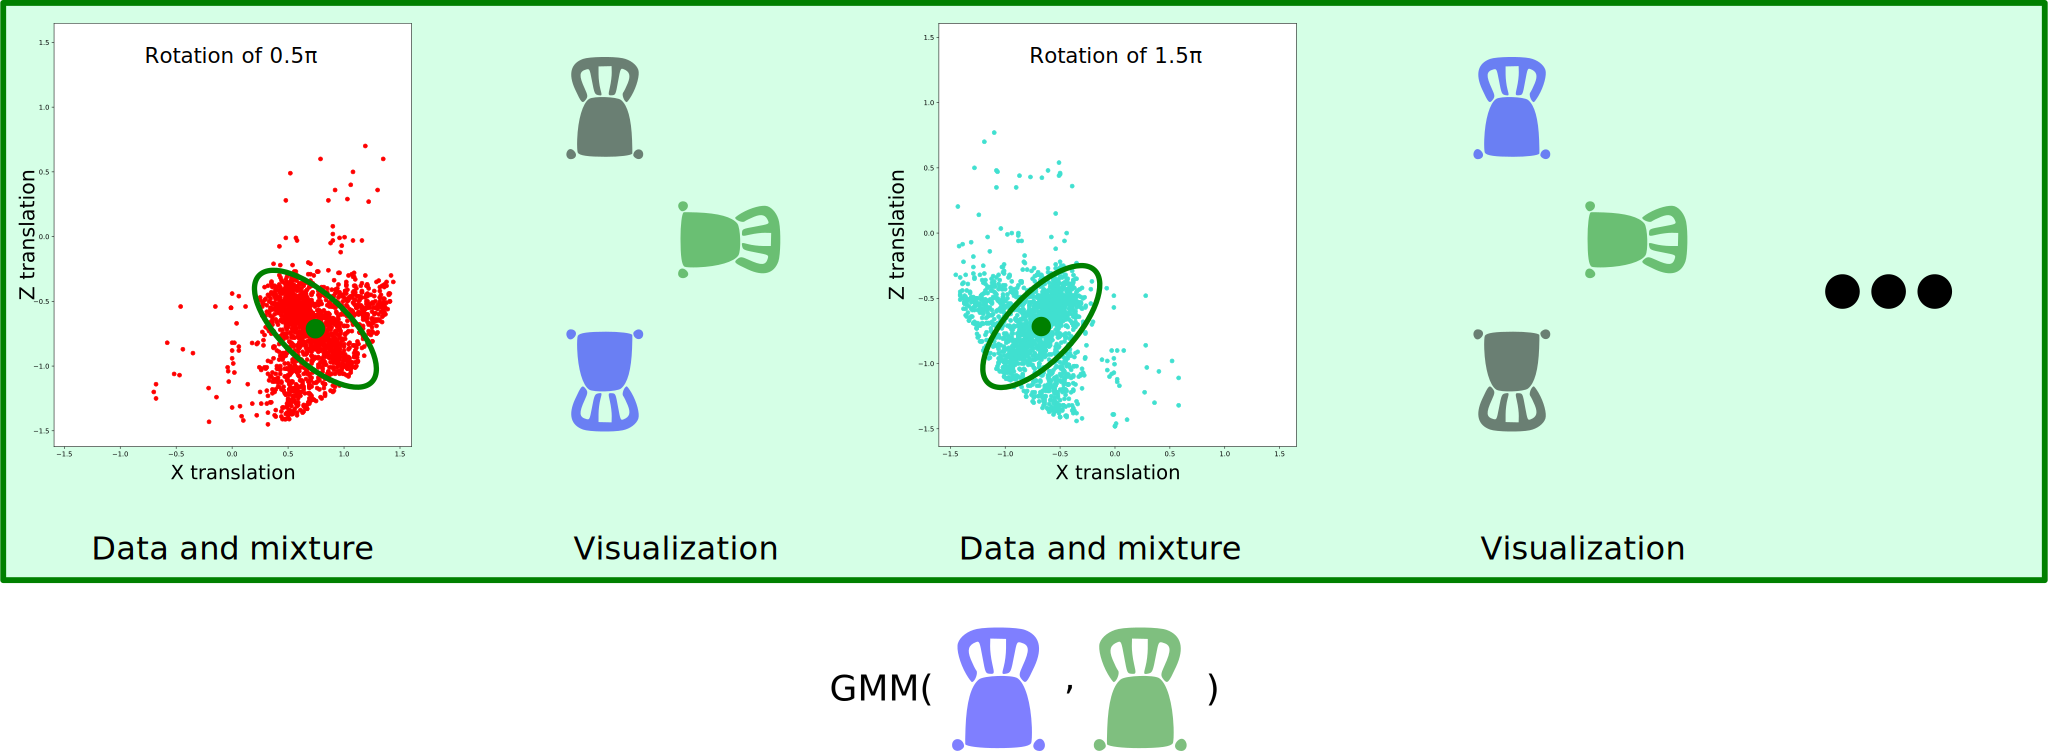
\includegraphics[width=\linewidth]{figures/mixture_components/mixture_components}
    \caption[Mixture components]{A visualization of two of the mixture components resulting from fitting the GMM to the relative transformations of pairs of chairs in the PBRS dataset. The means and standard deviational ellipses are plotted in green.}
    \label{fig:ch4:mixture_components}
\end{figure}

\subsubsection{Graph optimization}
\label{ssec:ch4:graph_optimization}
We now need to prune our over-complete set of candidate placements using the
trained object co-occurrence model. We represent this task as a graph labeling
problem.  Each candidate placement represents a node in the graph, and takes on
a binary label representing whether or not that candidate placement is present
in the final mockup. Unary costs for each label stem from the keypoint location
maps, and pairwise costs stem from the scene statistics GMM.  See
Figure~\ref{fig:ch4:graph_example}.

\begin{figure}
    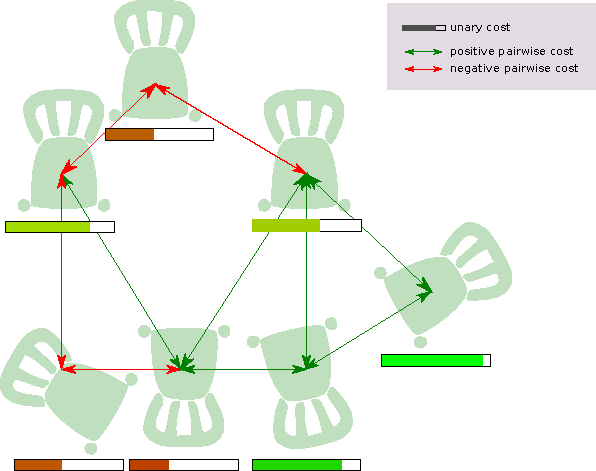
\includegraphics[width=\linewidth]{figures/graph_example/graph_example}
    \caption[Candidate selection visualization]{We model our candidate selection problem as a graph labeling problem, where the unary costs are based on the keypoint location maps, and the pairwise costs on the scene statistics GMM.}
    \label{fig:ch4:graph_example}
\end{figure}

\paragraph{Unary cost} To compute the unary score of a candidate placement $o_i \in \bb{O}$,
we \emph{generate} the keypoint location map $\bb{n}$ of $o_i$ (in the same
way we would do for creating a ground truth keypoint map) and compare it with
the keypoint location map $\bb{m}$ of the input image $\bb{x}$.  As we do not expect a
single placement to explain the entire keypoint location map, we setup the score
as a multiplicative one, with the value only being dependent on the agreement
of the actual keypoints the placement $o_i$ exhibits:
%
\[ u_i = \frac{\|\bb{n} \odot \bb{m}\|_F}{\bb{n} \odot \bb{n}}, \]
%
where $\|\cdot\|_F$ represents the Frobenius norm, and $\odot$ represents the Hadamard product.

The normalization factor ensures that a candidate that perfectly matches the
keypoint location map of our input image $\bb{x}$ gets a score of 1.  Finally, for a specific
candidate $o_i \in \bb{O}$, interpreting $u_i$ as a probability we get unary costs based on the log odds of $u_i$:
\begin{align}
    U_i(0) &= 0 \\
    U_i(1) &= -\log\left(\frac{u_i^\alpha}{1 - u_i^\alpha}\right)
\end{align}
where $\alpha$ is a scaling parameter to set the sensitivity of optimization to
the value in the keypoint maps. Our choice for the log odds means that a (scaled) score
of higher than $0.5$ results in a candidate unary cost that \emph{decreases} the score of the total
cost when selected, and otherwise \emph{increases} it.

\paragraph{Pairwise cost} The pairwise cost is based entirely on the fitted GMM. We extract
the relative translation $\bb{\delta}_t$ and orientation $\delta_\theta$, and evaluate
the trained GMM to get our raw pairwise score:
\[ p_{ij} = GMM(o_i, o_j). \]
The final pairwise score is then again based on the log odds corresponding to $p_{ij}$. It only applies when two objects co-occur:
\begin{align}
    P_{ij}(0, 0) &= P_{ij}(1, 0) = P_{ij}(0, 1) = 0 \\
    P_{ij}(1, 1) &= -\log\left(\frac{p_{ij}^\beta}{1 - p_{ij}^\beta}\right)
\end{align}
with $\beta$ a scaling parameter similar to $\alpha$.

Finally, we add an infinite pairwise cost to all candidate placement pairs that
intersect. These intersections are precomputed based on triangle-triangle
intersections.

We solve the final problem setup using OpenGM~\cite{OpenGM} by converting it to
a linear program and feeding it to CPLEX~\cite{CPLEX}.

\subsection{Iterative optimization}
\label{sec:ch4:iteration}
After the optimization from Section~\ref{sec:ch4:optimization} is complete, we
could stop and pass on the candidate placements with label 1 to the model
selection stage (Section~\ref{sec:ch4:model_selection}).  However, now that
some objects have been definitely placed, we can use this information to
improve our candidate generation step, and by extension our candidate selection
step. In other words, we iterate the process of candidate generation and
selection, using the newly selected candidates in each iteration as a strong prior for the
candidate generation process of the next generation.

\subsubsection{Added pairwise cost in generation step}
To take into account the already selected placements during the candidate
generation phase, we keep our original non-linear least squares optimization,
but to the loss function of each stage of the two stage process (see
Section~\ref{sssec:ch4:template_fitting}) we add a term that represents the
GMM.  Incorporating all mixture components in this
term is hard, as it is challenging to define a well-behaved objective function to minimize that
represents them. As noted by Olson et al.~\cite{Olson:2013:IJRR}, the
structure of the negative log-likelihood (NLL) of a GMM does not lend itself to
non-linear least squares optimization. Instead, they propose to approximate the
NLL of the full GMM by considering it as a Max-Mixture, reducing the NLL to the
weighted distance to the closest mixture mean (see Figure~\ref{fig:ch4:max_mixture} and \cite{Olson:2013:IJRR} for
details).  In fact, in our case it makes sense to only optimize with respect to
the closest mean, and not all means: a chair should either be encouraged to be
next to another chair, or opposite, but never both. This replaces the original GMM likelihood function
%
\[ p_\mathrm{GMM}(\bb{\delta}) = \sum_i w_i N(\bb{\mu}_i, \bb{\Sigma}_i) \]
%
with the Max-Mixture likelihood function
%
\[ p_\mathrm{Max}(\bb{\delta}) = \max_i w_i N(\bb{\mu}_i, \bb{\Sigma}_i), \]
%
where $\bb{\delta} = \begin{bmatrix} \bb{\delta}_t \\ \delta_\theta
\end{bmatrix}$ is the relative translation and orientation of the new candidate
w.r.t. the already placed object, and $w_k$ is the weight of the $k$th mixture in
the model.

Taking the negative log likelihood gives 
%
\[ -\log(p_\mathrm{Max}(\bb{\delta})) = \min_k \frac{1}{2} (\bb{\delta} - \bb{\mu}_k)^T \bb{\Sigma}_k^{-1}(\bb{\delta} - \bb{\mu}_k) - \log(w_k\eta_k), \]
%
where $N(\bb{\mu}, \bb{\Sigma})$ represents the normal distribution, and $\eta_k$ is the Gaussian normalization factor for the $k$th mixture. At
optimization time, during each step we find the mixture component $k^*$ that
minimizes this function, and then optimize w.r.t. the negative log likelihood
of the Gaussian of that component alone, resulting in the following term to be added to the objective function:
\[ \frac{1}{2} (\bb{\delta} - \bb{\mu}_{k^*})^T \bb{\Sigma}_{k^*}^{-1}(\bb{\delta} - \bb{\mu}_{k^*}). \]

By decoupling the component selection from the optimization step, we've
restored the nice properties of the single Gaussian negative log likelihood.
This term is added for each already placed object.

\begin{figure}
    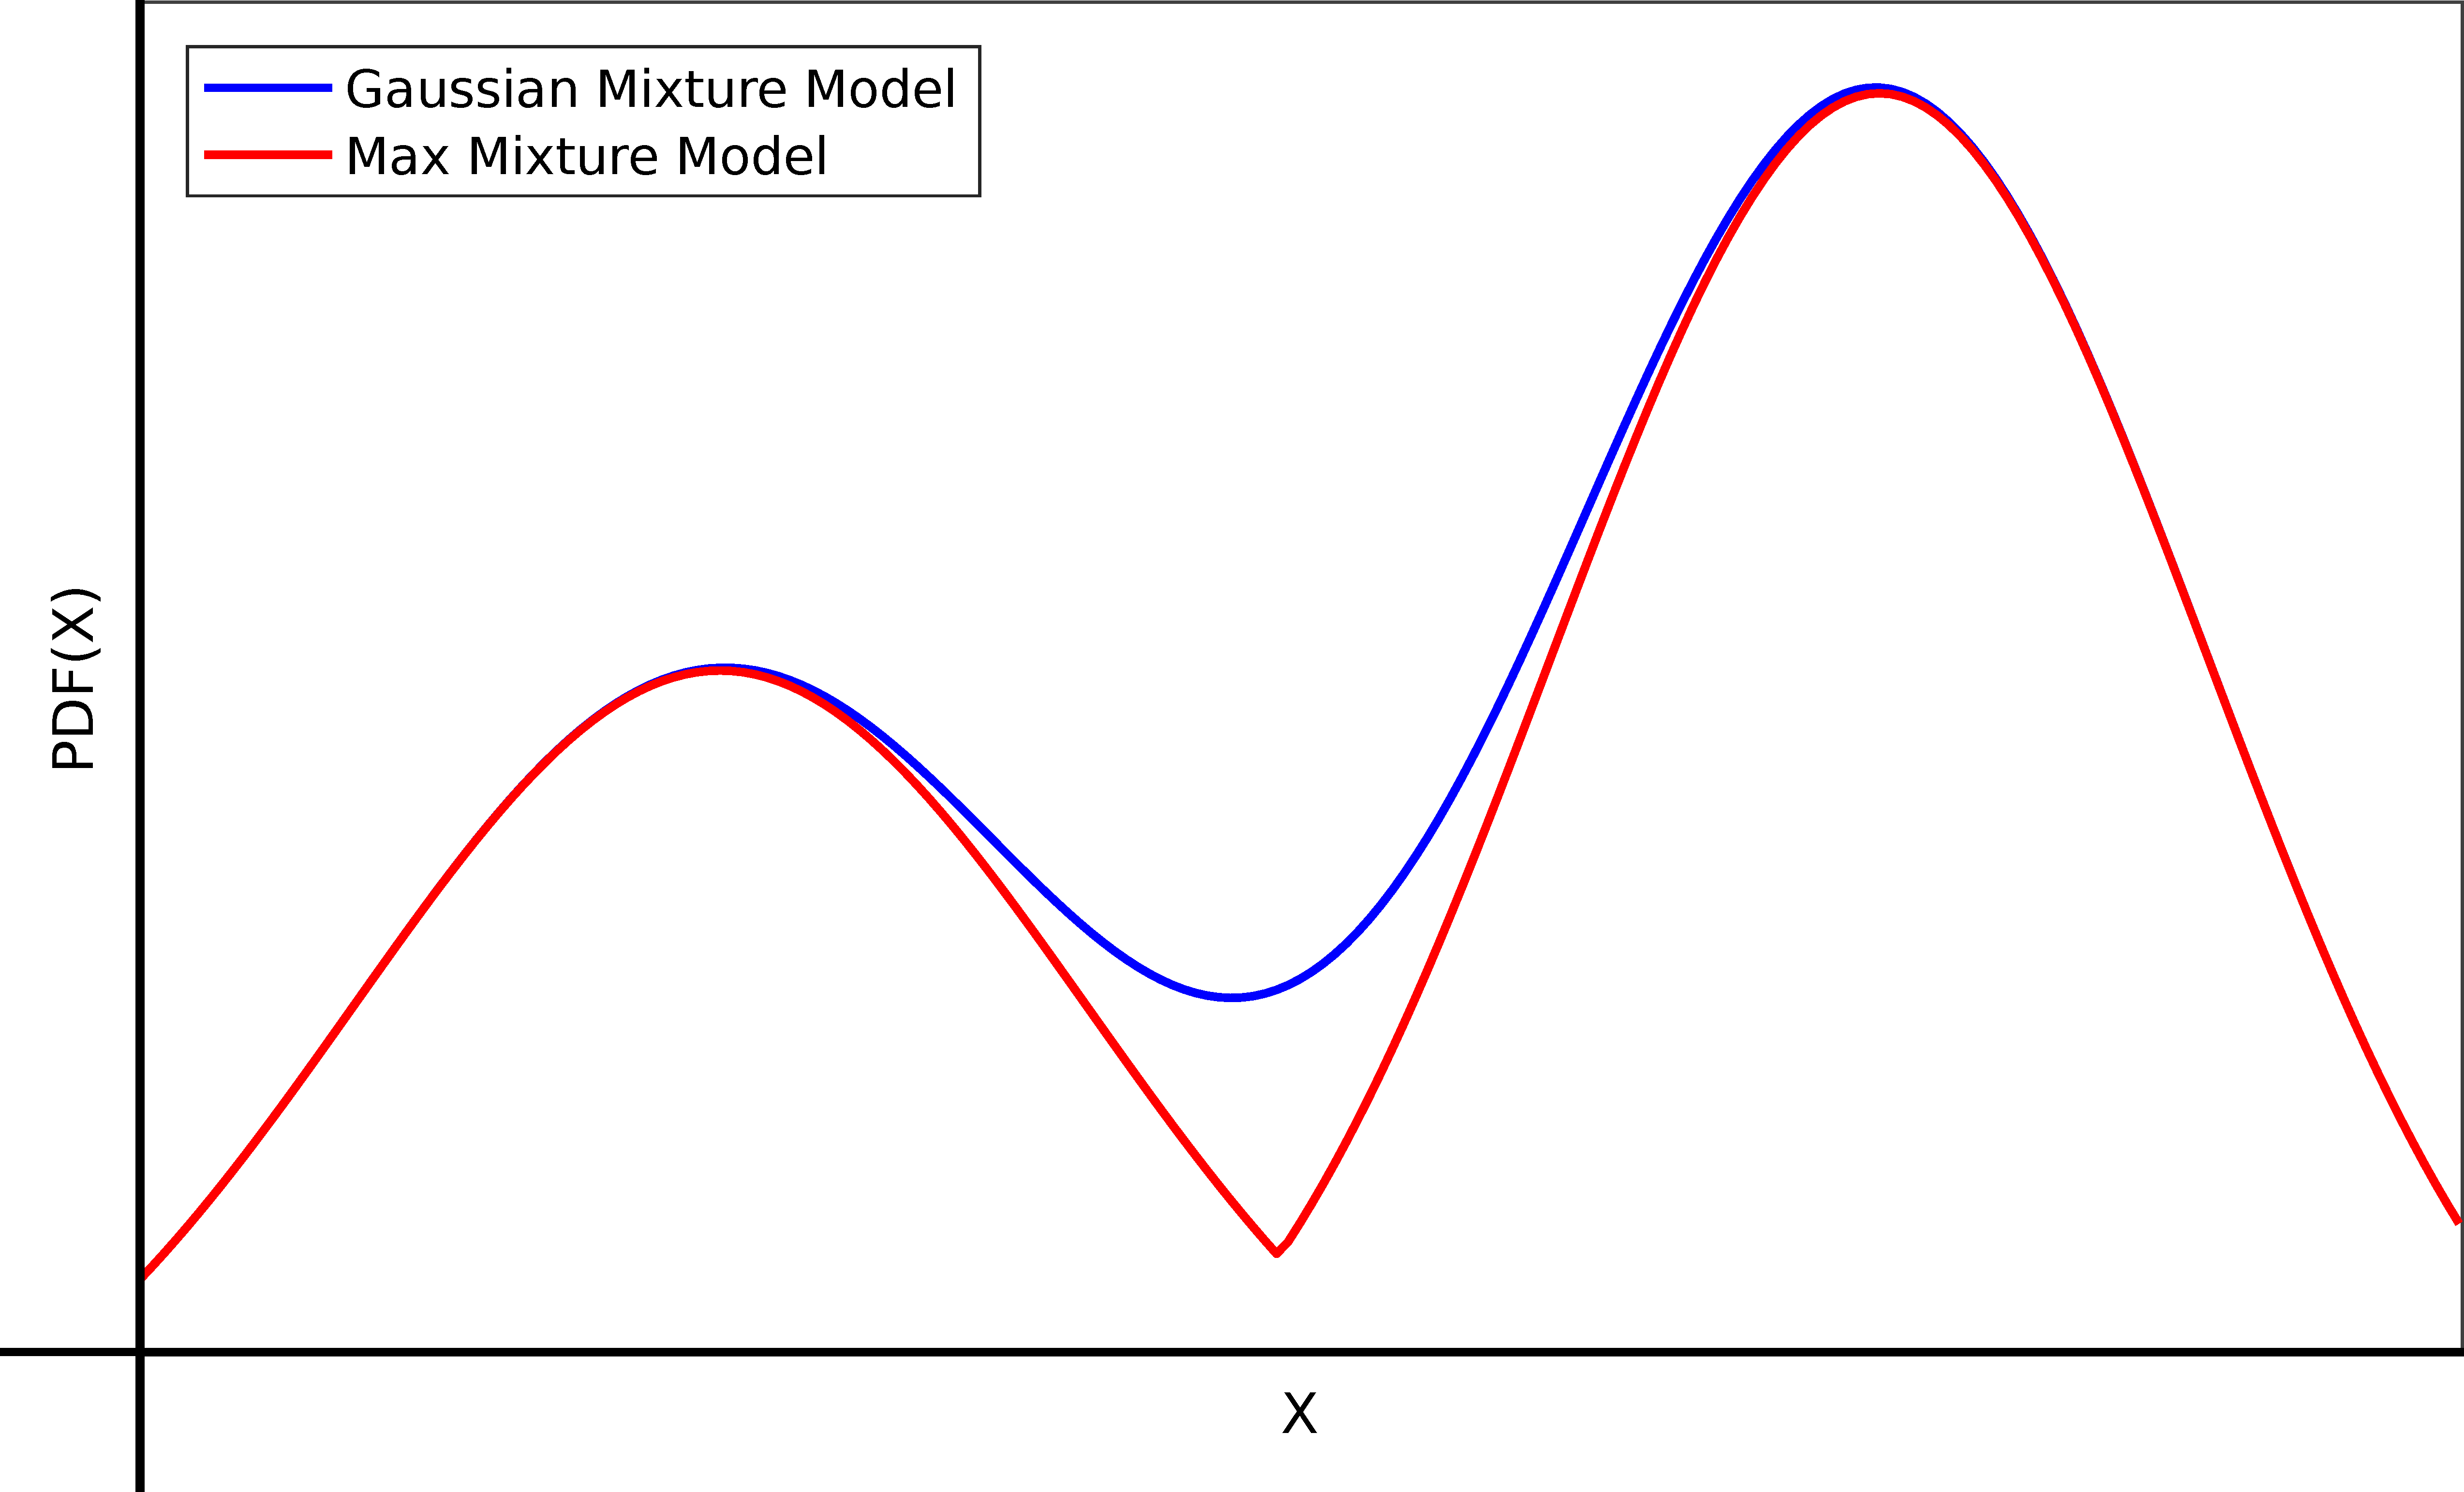
\includegraphics[width=\linewidth]{figures/max_mixture/max_mixture}
    \caption[Max mixture model]{We approximate the GMM using a Max-Mixture Model from Olson et al., 2013~\cite{Olson:2013:IJRR}. Due to the simplified negative log likelihood of this model we can then use it in our non-linear least squares optimization.}
    \label{fig:ch4:max_mixture}
\end{figure}

\subsubsection{Added unary cost in selection step}
As the already selected placements are not part of the optimization during later iterations,
the influence of the GMM on a new candidate placement w.r.t. already selected placements becomes
a unary cost. So, for each candidate placement in the second iteration, we add a term to $U_i(1)$
w.r.t. each of the already selected placements:
%
\[ -\log\left(\frac{GMM(o_i, o^*_j)^\beta}{1 - GMM(o_i, o^*_j)^\beta}\right). \]
%
With these modifications, the candidate generation step and candidate selection
step are iterated until convergence, i.e. until no new objects are added to the
scene.

\subsection{Model selection}
\label{sec:ch4:model_selection}
The set of all selected placements still only consist of template parameters, not actual chair models.
As a final step, we find the chair $g^*$ in our database $\bb{M}$ that best fits the
template. To do so, we reproject the 3D keypoint coordinates of each chair in
the database to the PCA coordinate space, and find the chair whose PCA
coordinates are closest to the PCA coordinates of our template:
%
\[ g^* = \arg\min_{g \in \bb{M}} \|[\mathrm{PCA(g)}]_0^3 - \bb{p}\|^2, \]
where $\bb{p}$ are the PCA coordinates of the candidate's template.
%
The resulting chair models together with their transform constitute our final scene mockup.

\subsection{Hyper parameters}
Our optimization pipeline depends on a number of hyper parameters. We optimized
these using HyperOpt~\cite{HyperOpt}, which employs a Tree of Parzen Estimators (Bergstra et al., 2013~\cite{Bergstra:2013:ICML}).
As our objective function we used the PercCorrectFull measure (see Section~\ref{sec:ch4:performance_measures}).
As ground truth data we used 10 scenes we annotated specifically for this purpose,
in the same way as the data used for evaluation (see Section~\ref{sec:ch4:ground_truth_annotation}).
See Table~\ref{tab:ch4:hyperparameters} for a list of resulting hyper parameter values.

\begin{table}
    \centering
    \resizebox{\linewidth}{!}{
        \begin{tabular}{|c|c|c|}
            \hline
            Name     & Description                               & Value \\ \hline
            $\alpha$ & Sensitivity of keypoint maps              & 0.61  \\ \hline
            $\beta$  & Sensitivity to object co-occurrence model & 0.14  \\ \hline
            $\tau_m$ & Lower threshold of keypoint location map  & 0.25  \\ \hline
            $\tau_u$ & Maximum cost for selecting candidate      & 0.21  \\ \hline
        \end{tabular}
    }
    \caption[Hyper parameters]{Hyper parameters of optimization, found by HyperOpt~\cite{HyperOpt}}
    \label{tab:ch4:hyperparameters}
\end{table}

\subsection{Data}
\label{sec:ch4:training_data}
\subsubsection{Image data}
For purposes of qualitative evaluation, we scraped the
interior design website~\cite{Houzz} for the top 1000 results of the search
query ``dining room''. We denote this dataset \textsc{Houzz}.  These images are
high quality and represent difficult but fair scenarios on which we expect our
method to perform well. Some examples of these images can be seen in
Figure~\ref{fig:ch4:houzz}.

\begin{figure}
    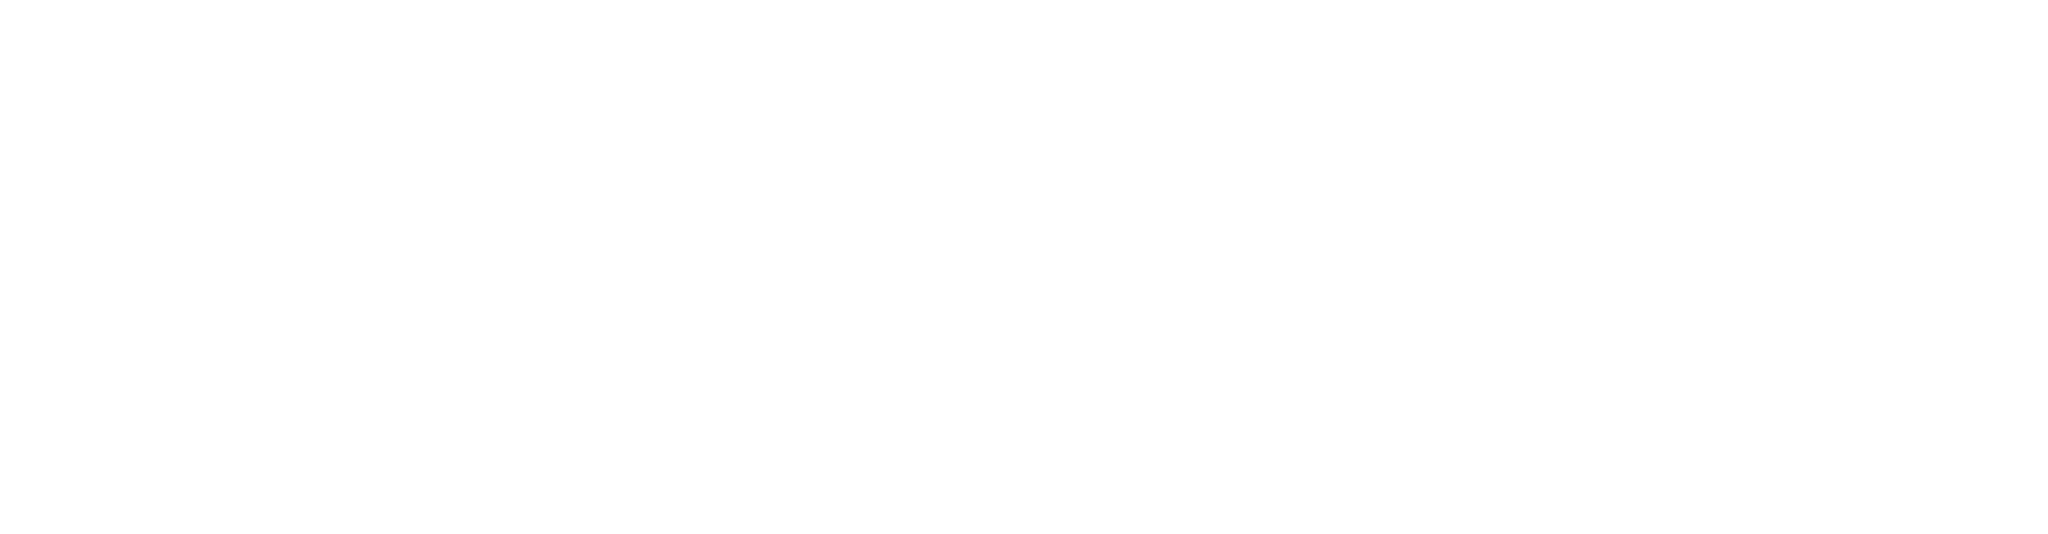
\includegraphics[width=\linewidth]{figures/houzz_example/houzz_example}
    \caption[Houzz samples]{Example images from our scraped \textsc{Houzz} dataset.}
    \label{fig:ch4:houzz}
\end{figure}

\subsubsection{Network training data}
Traditionally, training a deep neural network requires a large amount of
training data.  To our knowledge, there is no known large dataset of
photographs accurately annotated with object keypoints. As such, we resort
to creating our own training data. Ideally, the training data should be
from the same distribution as our intended testing data, i.e.\ photographs
of indoor scenes. However, creating a large-scale dataset of this type
is extremely time-consuming and expensive. On the other hand, synthetic
data in the form of realistic 3D indoor scenes along with physically-based
renders is already available in high numbers \cite{Zhang:2017:CVPR}.
Still, despite the high quality of the renders, there is still a significant
discrepancy between the feature distribution of the renders and that of the
photographs. As such, we augment the synthetic dataset with a subset of real
photographs from \textsc{Houzz} annotated through Amazon Mechanical Turk. We
now discuss each data type in turn.

\paragraph{Synthetic data}
The dataset provided by Zhang et al.~\cite{Zhang:2017:CVPR} provides 45K realistic indoor
scenes, and 400K physically-based renders of these scenes (see Figure~\ref{fig:ch4:pbrs}). We denote this
dataset as \textsc{PBRS}. These scenes consist of a fixed set of 2500 different
models across 60 classes. Among these models there are $\pm250$ chairs. We took a
subset of 100 of these chairs and annotated them with our previously selected
keypoint types. We then took all renders that contain at least 1 of the
annotated chairs and reprojected the keypoint locations into these renders,
yielding one image/keypoint map pair as training data per render. This resulted
in a set of $\pm8000$ image/keypoint map pairs in total.

\begin{figure}
    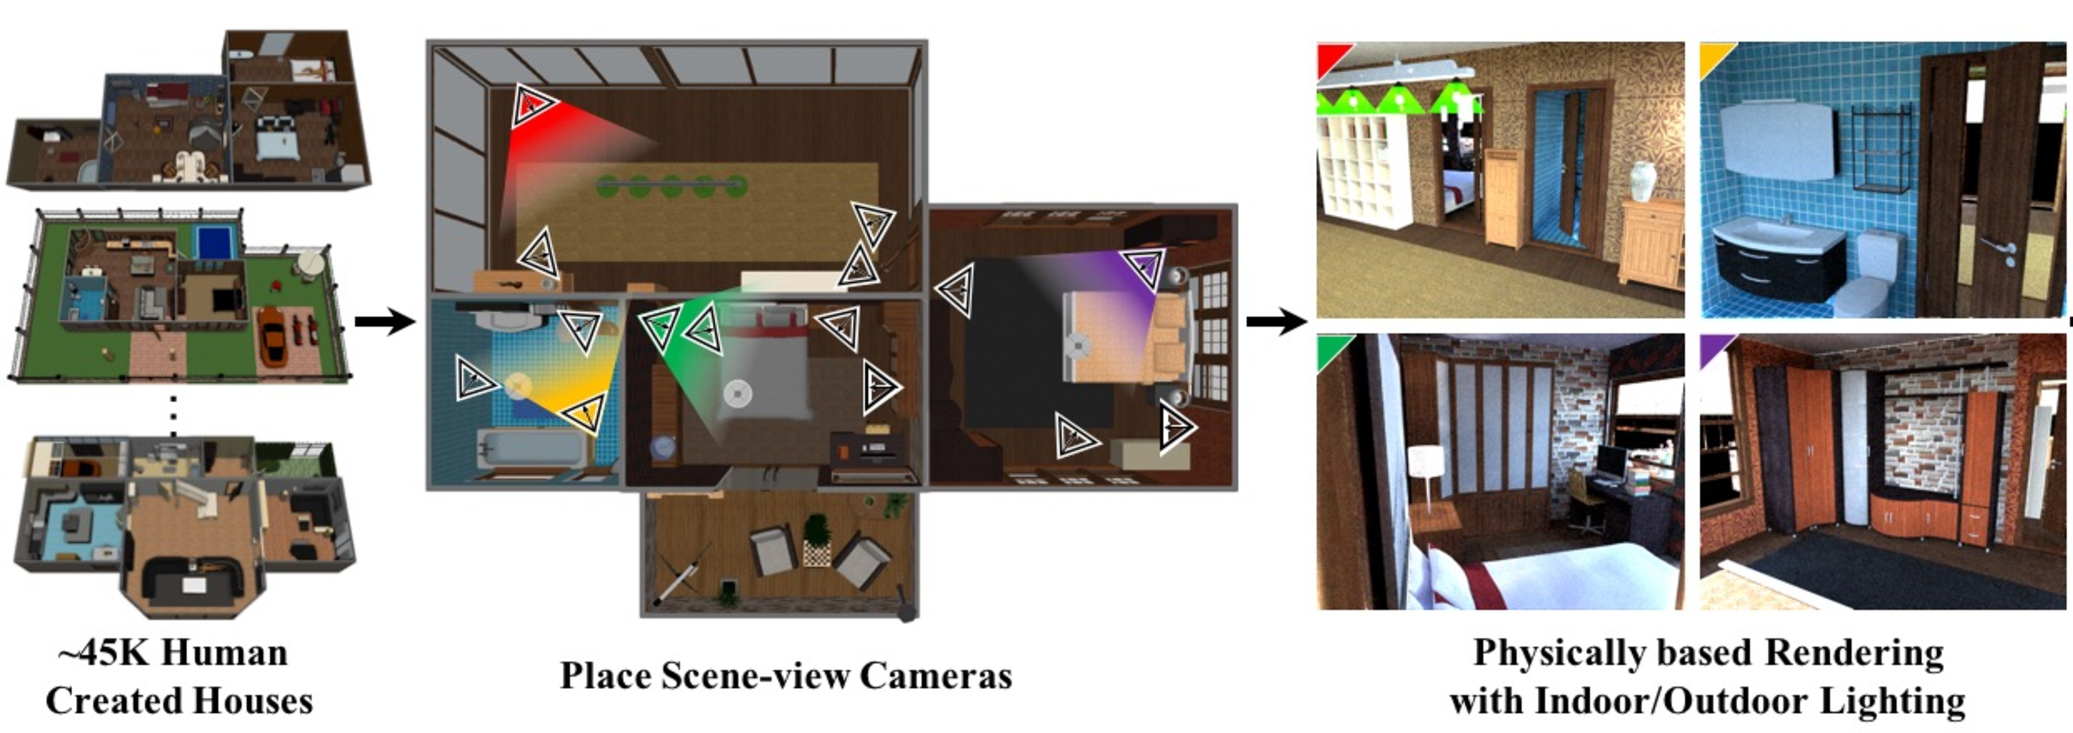
\includegraphics[width=\linewidth]{figures/pbrs/pbrs}
    \caption[PBRS dataset]{For the training setup of our network with synthetic data, we use renders from the PBRS dataset~\cite{Zhang:2017:CVPR}, which provides $\pm$45K houses with $\pm$400K high quality renders. Figure from \cite{Zhang:2017:CVPR}.}
    \label{fig:ch4:pbrs}
\end{figure}

\paragraph{Real data}
Unfortunately, the synthetic data alone does not result in good performance on
real data. Two distinct reasons can be identified. First, even though the renders
in \textsc{PBRS} are of high quality, their feature distribution is both
distinct from real photographs as well as less diverse. Secondly, at the time
of writing, the set of renders and the set of scenes available for
\textsc{PBRS} had some discrepancies between them, resulting in a small but
significant set of renders that do not agree with the automatically generated
keypoint maps.

To address both of these issues, we annotated a subset of 500 images from the
\textsc{Houzz} dataset through Amazon Mechanical Turk. We asked 3 workers per
image to annotate all keypoints in the image through a drag-and-drop interface
(see Figure~\ref{fig:ch4:amt}), and averaged the resulting 3 keypoint maps per
image.  This resulted in a training set of 500 hand-annotated photographs, which
was then used to train our keypoint estimation network.

\begin{figure}
    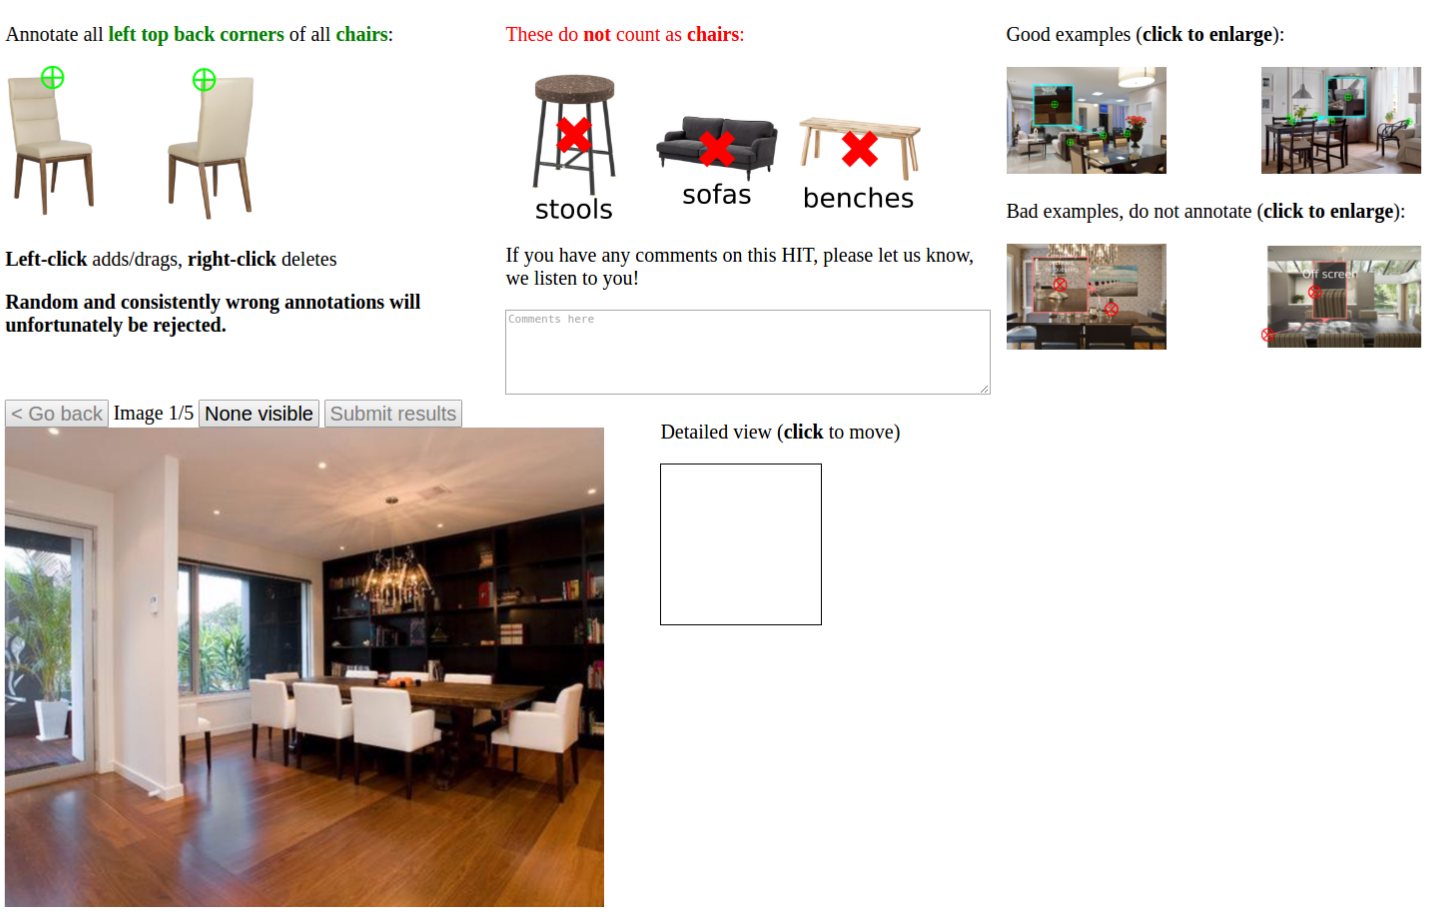
\includegraphics[width=\linewidth]{figures/amt/amt}
    \caption[MTurk interface]{The Amazon MTurk interface we used to annotate 500 photographs with keypoints.}
    \label{fig:ch4:amt}
\end{figure}

\paragraph{Final training set} We experimented with 3 different training setups.
In the first setup, we trained the network only with synthetic data. In the second setup,
we only trained the network with real data. Finally, in the third setup, we 
first trained the network until convergence with the synthetic data,
and then finetuned the network using the smaller set of real data.

Surprisingly, the best performance on the test set resulted from setup 2, i.e.
training only with the real data. Apparently, the shortcomings of the synthetic
data mentioned above were of higher importance than expected. One likely
explanation is the fact that training the network with the synthetic data first
steers away the network weights from those that were the result of the ImageNet
pretraining, which already encompass a high general understanding of real
photographs. The numbers show that this initial information is more valuable than the
extent of the synthetic data as well as its structural similarity to our test
data.

\subsubsection{Model data} The models annotated for the purpose of generating
synthetic network training data also immediately function as our model set
$\bb{M}$.

\section{Evaluation}
\label{sec:ch4:evaluation}
We thoroughly evaluated our method, investigating the importance of each part
of our pipeline as well as comparing our results with other methods.  We will
first discuss the creation of a set of ground truth annotated scenes for the
purpose of quantitative evaluation (Section~\ref{sec:ch4:ground_truth_annotation}). We then define
a set of diverse performance measures (Section~\ref{sec:ch4:performance_measures}), after which we introduce two baseline methods for comparison purposes (Section~\ref{sec:ch4:baselines}). We evaluate our method with the ground truth set,
and compare the numbers with two distinct baseline methods (Section~\ref{sec:ch4:comparison}). Finally, we perform
an ablation study to show the influence of each on the final performance (Section~\ref{sec:ch4:ablation}). Both
quantitative and qualitative results will be shown along the way.

\subsection{Ground truth annotation}
\label{sec:ch4:ground_truth_annotation}
In order to quantitatively measure the performance of both the baseline methods
and our own, we need a set of ground truth annotated scenes, i.e. images for
which all objects have been placed manually.  We setup an application in which
an object can be placed by clicking and dragging, as well as by annotating a
number of keypoints of the object and optimizing for its location and scale.
Moreover, objects can be copied and translated along their local coordinate
axes, allowing for quick and precise annotation (see
Figure~\ref{fig:ch4:gt_annotation}). We use the automatically estimated camera
parameters, making sure we discard any scenes for which the camera estimation
is completely off.  We used this tool to fully annotate 100 scenes, which were
randomly selected from our \textsc{Houzz} dataset of 1000 images.

\begin{figure}
    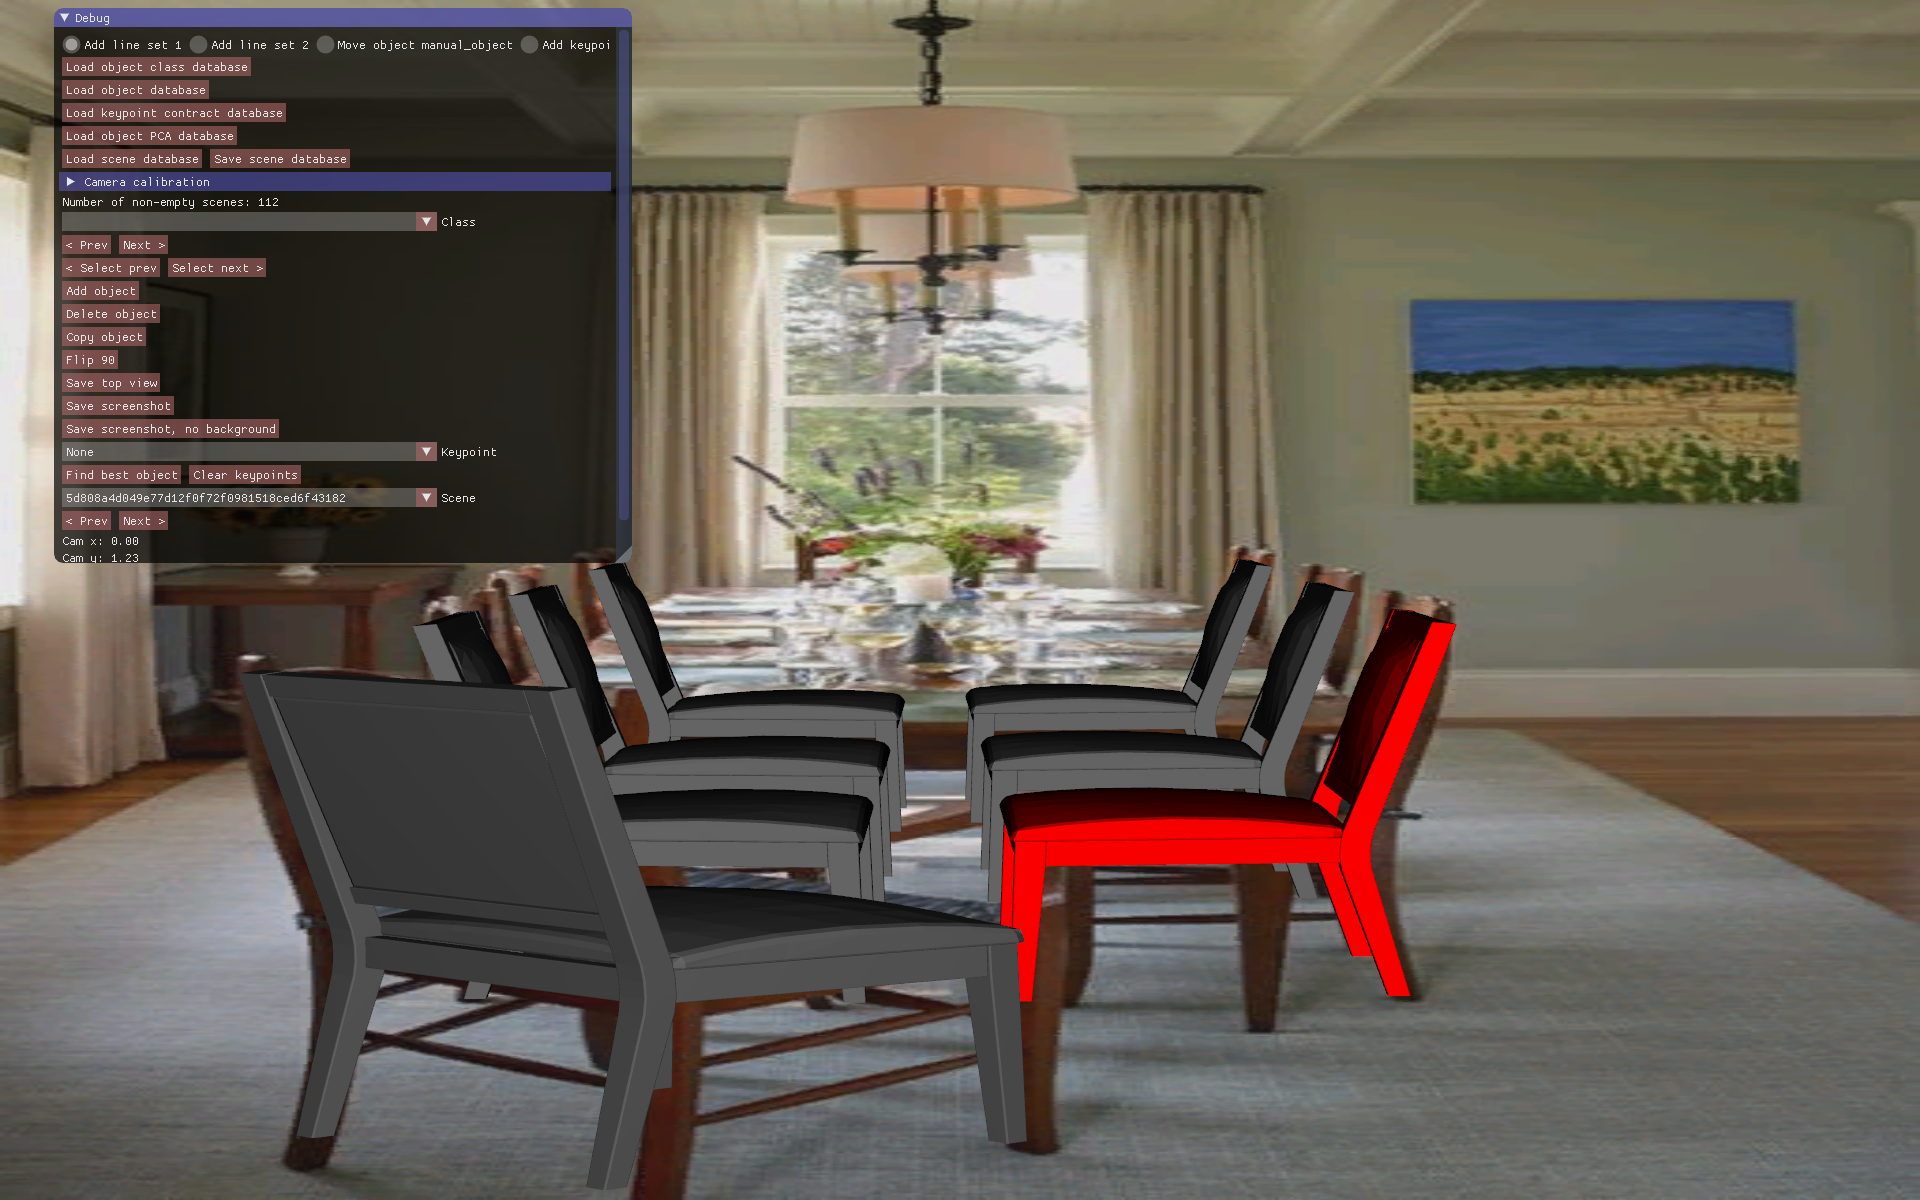
\includegraphics[width=\linewidth]{figures/groundtruth_annotation/groundtruth_annotation}
    \caption[Annotation tool]{We created a ground truth annotation tool for quickly creating ground truth scene mockup examples.}
    \label{fig:ch4:gt_annotation}
\end{figure}

\subsection{Performance measures}
\label{sec:ch4:performance_measures}
A scene mockup method can be quantitatively evaluated in many different ways.
As no single measure tells the full story, we have opted for a number of
different ones. 

\paragraph{Notation} We will use the concept of ``source'' and ``target''
to denote the two scenes between which some measure is computed. We
specifically do not use ``result scene'' and ``ground truth scene'', because
they can act as either source or target scene in most measures. We denote
the objects in the source and target scene as $o_S \in \bb{S}$, $o_T \in \bb{T}$
respectively.  $J_3(o_S, o_T)$ and $J_2(o_S, o_T)$ represent the Jaccard index
or \emph{intersection-over-union} (IoU) of the bounding boxes of $o_S$ and
$o_T$ in 3D world space and 2D screen space respectively (see Figure~\ref{fig:ch4:iou}). Finally, given an
object $o_S$ we define the ``$J_i^*$ correspondence'' with $\bb{T}$ as the object in
$T$ with the maximum Jaccard index with $o_S$: \[ J_i^*(o_S, \bb{T}) = \arg\max_{o_T \in \bb{T}}
J_i(o_S, o_T) \]
Intuitively, this returns, for a given object, the "best matching" object from
the other scene in terms of overlap.
\begin{figure}
    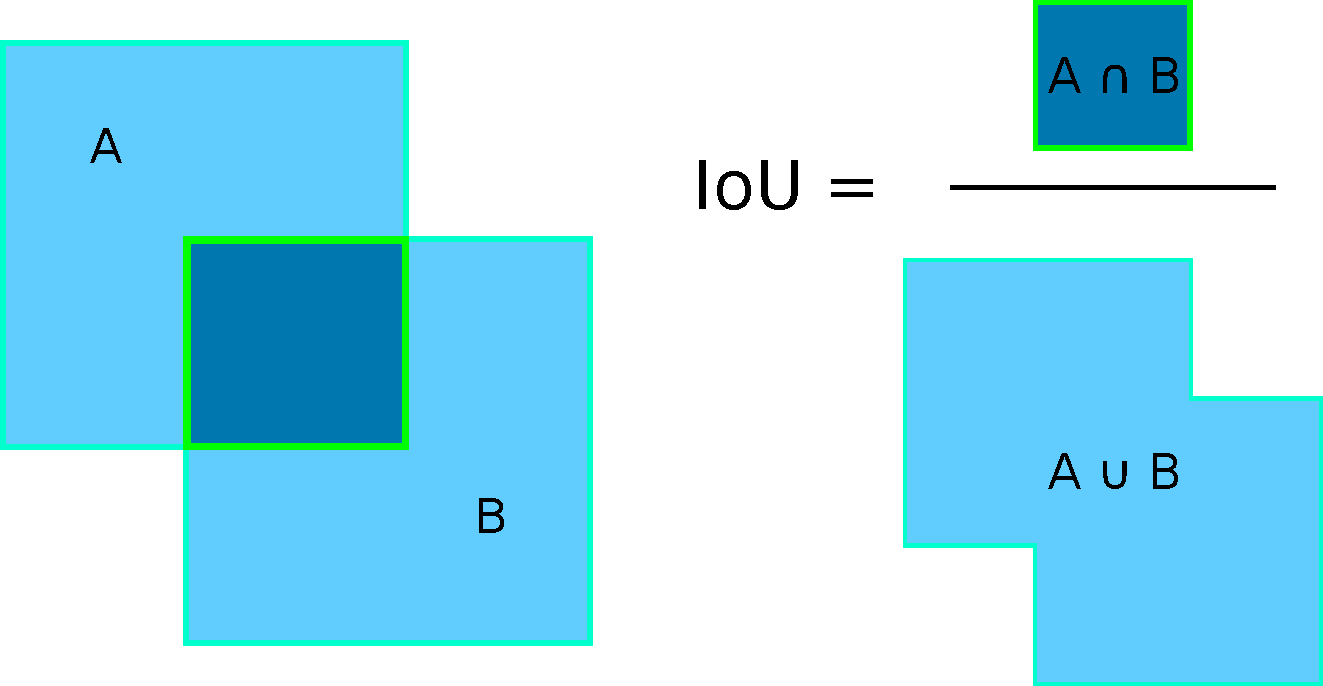
\includegraphics[width=\linewidth]{figures/iou/iou}
    \caption[Intersection-over-union visualization]{Visualization of the intersection-over-union measure in 2D.}
    \label{fig:ch4:iou}
\end{figure}
\begin{description}\itemsep0pt
    \item[Average Max IoU] This measure takes a source scene and a target
        scene, and records the accuracy with which the volumes of the objects
        in the source scene agree with the objects in the target scene.
        Specifically, for each object in the source scene, we record the IoU of
        the object with its MaxIoU correspondence.  This measure is averaged
        over all objects in the source scene to produce the final measure. 

        \[ \mathrm{AvgMaxIoU}(\bb{S}, T) = \frac{1}{|\bb{S}|} \sum_{o_S \in \bb{S}} J_3(o_S, J_3^*(o_S, \bb{T})) \]

        We measure in both directions, i.e. with the ground truth as source and
        result as target, as well as vice versa.  The former can be thought of
        as a form of ``recall'' and the latter as a form of ``precision''. This
        measure is angle-agnostic and captures the location similarity of objects in the source
        scene w.r.t. those in the target scene.
    \item[Percentage correct location] This measure takes a source scene and a
        target scene, and records the percentage of objects in the source scene
        that have a $J_3^*$ correspondence over a certain threshold
        $\tau_{J}$. To define it, we first set
        \begin{multline*}
            \mathrm{CorrectLoc}(\bb{S}, \bb{T}) = \\ \{ o_S \in \bb{S} \mid J_3(o_S, J_3^*(o_S, \bb{T})) > \tau_{J} \}.
        \end{multline*}
        Then,
        \[ \mathrm{PercCorrectLoc}(\bb{S}, \bb{T}) = \frac{|\mathrm{CorrectLoc}(\bb{S}, \bb{T})|}{|S|}. \]
        We again measure in both directions, yielding recall (ground truth is source, result is target)
        and precision (vice versa) measures.
    \item[Percentage correct] As the previous measure, but with the added constraint that the
        angle difference is under a threshold $\tau_{\theta}$. So,
        \begin{multline*}
            \mathrm{CorrectFull}(\bb{S}, \bb{T}) = \\ \{ o_S \in \mathrm{CorrectLoc}(\bb{S}, \bb{T}) \mid \angle(o_S, J_3^*(o_S, \bb{T})) < \tau_{\theta} \}. 
        \end{multline*}
        Then,
        \[ \mathrm{PercCorrectFull}(\bb{S}, \bb{T}) = \frac{|\mathrm{CorrectFull}(\bb{S}, \bb{T})|}{|\bb{S}|}. \]
    \item[Angle difference] This measures the average angle difference for the objects that have
        correct location. This measure is symmetrical.
        \begin{multline*}
            \mathrm{AngleDiff}(\bb{S}, \bb{T}) = \\ \frac{\sum_{o_S \in \mathrm{CorrectLoc}(\bb{S}, \bb{T})} \angle(o_S, J_3^*(o_S, \bb{T}))}{|\mathrm{CorrectLoc}(\bb{S}, \bb{T})|}
        \end{multline*}
    \item[Average Max 2D IoU] This measures the average maximum IoU of the
        bounding boxes of each projected object in the source scene with the
        bounding boxes of the projected objects in the target scene.
        \[ \mathrm{AvgMax2DIoU}(\bb{S}, \bb{T}) = \frac{1}{|\bb{S}|} \sum_{o_S \in \bb{S}} J_2(o_S, J_2^*(o_S, \bb{T})) \]
\end{description}

\subsection{Baseline methods}
\label{sec:ch4:baselines}
We compare our method with two baselines from the literature. As the exact problem
formulation we employ has to our knowledge not been attempted, we convert the output
of each baseline (in both cases 3D pose but 2D, image space locations of chairs) to
the 3D scene mockup format that our method produces.

\begin{figure}[h!tb]
    \centering
    \def\svgwidth{\linewidth}
    \import{figures/baseline_example/}{baseline_example.pdf_tex}
    \caption[Baseline output]{Example of raw output of the two baseline methods.}
    \label{fig:ch4:baseline_example}
\end{figure}

\paragraph{Seeing chairs~\cite{Aubry:2014:CVPR}} This method from Aubry et al. finds chairs by
matching so-called ``discriminative visual elements'' or DVEs from a set of
rendered views of 1000+ chair models with the input image. These DVEs are
linear classifiers over HOG features \cite{Dalal:2005:CVPR} learnt from the
rendered views in a discriminative fashion. They are learned at multiple scales,
and only the most discriminative ones are kept for matching purposes. At test time,
a patch-wise matching process finds the best-matching image patch/rendered patch pairs,
and then finds sets of pairs that come from the same rendered view (see Aubry et al.'s paper for details~\cite{Aubry:2014:CVPR}).

This method outputs scored image space bounding boxes together with a specific
chair model and pose. See Figure~\ref{fig:ch4:baseline_example}, left. For the 3D
performance measures (Section \ref{sec:ch4:performance_measures}) we need the
output in the form of a 3D scene. To this end we convert each set of bounding
box, pose, and chair model to a 3D scene. As the camera is known
(Section~\ref{sec:ch4:camera_estimation}), we can optimize the location (in the
X-Z plane) of the 3D model without changing its pose, such that the 2D bounding
box of the projected model matches as closely as possible with the detected
bounding box. This can be formulated as a least-squares optimization problem,
which we solve using Ceres~\cite{Ceres}.

\paragraph{FasterRCNN~\cite{Ren:2015:NIPS} + 3D-INN~\cite{Wu:2016:ECCV}} This
baseline is a combination of a convolutional neural network (CNN) trained for
object detection (FasterRCNN) and another CNN trained for 3D object interpretation
(3D-INN). We use FasterRCNN to extract bounding boxes of chairs from the input
image, and then feed these regions of interest to 3D-INN, which produces a
templated chair model consisting of a set of predefined 3D keypoints as well as
a pose estimate (azimuth and elevation).  See Figure~\ref{fig:ch4:baseline_example}, right. 
The set of keypoint types we have chosen for our method is a subset of the keypoints
produced by 3D-INN, and thus we can use the candidate generation part of our pipeline (see Section~\ref{sec:ch4:candidate_generation})
to convert the extracted keypoints to a 3D chair.


\subsection{Comparison}
\begin{figure*}[h!tb]
    \centering
    %\def\svgwidth{\linewidth}
    %\import{figures/qualitative_results/}{qualitative_results.pdf_tex}
    \includegraphics[width=\linewidth]{figures/qualitative_results/qualitative_results.pdf}
    \caption[Qualitative results]{Qualitative results for our method vs. the baseline methods.}
    \label{fig:ch4:qualitative_results}
\end{figure*}

\label{sec:ch4:comparison}
\begin{table*}[h!]
    \resizebox{\linewidth}{!}{
        \begin{tabular}{|c|c|c|c|c|}
        \hline
                                                                      & AvgMaxIoU (precision)   & AvgMaxIoU (recall)   & AvgMaxIoU (F1)   & \\ \hline
        3D-INN~\cite{Wu:2016:ECCV} + FasterRCNN~\cite{Ren:2015:NIPS}  & 0.316                   & 0.150                & 0.198            & \\ \hline
        SeeingChairs~\cite{Aubry:2014:CVPR}                           & 0.195                   & 0.128                & 0.149            & \\ \hline
        Ours                                                          & \textbf{0.386}          & \textbf{0.250}       & \textbf{0.293}   & \\ \hline
                                                                      & PercCorrect (precision) & PercCorrect (recall) & PercCorrect (F1) & \\ \hline
        3D-INN~\cite{Wu:2016:ECCV} + FasterRCNN~\cite{Ren:2015:NIPS}  & 0.263                   & 0.124                & 0.165            & \\ \hline
        SeeingChairs~\cite{Aubry:2014:CVPR}                           & 0.071                   & 0.043                & 0.052            & \\ \hline
        Ours                                                          & \textbf{0.298}          & \textbf{0.167}       & \textbf{0.207}   & \\ \hline
                                                                      & PercCorrectFull (precision) & PercCorrectFull (recall) & PercCorrectFull (F1) & \\ \hline
        3D-INN~\cite{Wu:2016:ECCV} + FasterRCNN~\cite{Ren:2015:NIPS}  & 0.04                        & 0.015                    & 0.021                & \\ \hline
        SeeingChairs~\cite{Aubry:2014:CVPR}                           & 0.013                       & 0.007                    & 0.009                & \\ \hline
        Ours                                                          & \textbf{0.285}              & \textbf{0.161}           & \textbf{0.198}       & \\ \hline
                                                                      & AvgMax2DIoU (precision) & AvgMax2DIoU (recall) & AvgMax2DIoU (F1) & AngleDiff (in degrees) \\ \hline
        3D-INN~\cite{Wu:2016:ECCV} + FasterRCNN~\cite{Ren:2015:NIPS}  & 0.526                   & 0.336                & 0.401            & 55.8                   \\ \hline
        SeeingChairs~\cite{Aubry:2014:CVPR}                           & 0.372                   & 0.325                & 0.341            & 11.4                   \\ \hline
        Ours                                                          & \textbf{0.628}          & \textbf{0.470}       & \textbf{0.525}   & \textbf{7.3}           \\ \hline

        \end{tabular}
    }
    \caption[Quantitative performance]{Quantitative performance of our method vs. the two baseline methods. We outperform the baseline significantly across all measures.}
    \label{tab:ch4:performance}
\end{table*}
We ran our pipeline and the two baseline methods on the full ground truth
annotated scene set (Section~\ref{sec:ch4reddy.pradyumna5@gmail.com:ground_truth_annotation}). A sampling
of results can be seen in Figure~\ref{fig:ch4:qualitative_results}. The same visualization
for all 100 scenes in our ground truth set can be found in Appendix~\ref{app:results}.

The baseline methods perform well when there is no occlusion in the scene.
Chairs that are clearly visible are reconstructed reliably, as the visual
information directly available is enough for these methods to make a reasonable
inference about the object's pose and identity. However, when a chair is partly
occluded, these methods break down quickly. In contrast, our method is more
often able to recover from these situations, due to the incorporation of the
object co-occurrence model. 

This difference in performance is also reflected in the quantitative results. We
extracted the performance measures listed in
Section~\ref{sec:ch4:performance_measures} from each method, and list them in
Table~\ref{tab:ch4:performance}. Our method outperforms the baselines on all
counts.  Moreover, in Figure~\ref{fig:ch4:performance_changes} we show how the
PercCorrectFull measure changes under varying thresholds of IoU and angle (see
Section~\ref{sec:ch4:performance_measures}).

\begin{figure}[h!]
    \begin{subfigure}[t]{0.49\linewidth}
        \centering
        \def\svgwidth{\linewidth}
        \import{figures/performance_comparison/}{performance_perc_f1_angle_thresh.pdf_tex}
        \caption{Performance under varying $\tau_\theta$}
    \end{subfigure}
    \begin{subfigure}[t]{0.49\linewidth}
        \centering
        \def\svgwidth{\linewidth}
        \import{figures/performance_comparison/}{performance_perc_f1_iou_thresh.pdf_tex}
        \caption{Performance under varying $\tau_J$}
    \end{subfigure}
    \caption{Changes in performance under varied angle and IoU thresholds.}
    \label{fig:ch4:performance_changes}
\end{figure}


\subsection{Ablation study}
\label{sec:ch4:ablation}
Finally, we evaluated the importance of each of our pipeline's optional steps to the final performance. Specifically,
we ran our pipeline on the full test set under two weakening conditions. In the first condition, we disable all pairwise
costs, and run the entire pipeline based solely on the keypoint location maps. In the second condition, we only run
the second and third stage once, removing the possibility of the candidate generation stage benefiting from previously placed objects.
Results are found in Table~\ref{tab:ch4:ablation}.

There are some things to note. First, although AvgMaxIOU recall increases when disabling scene statistics, the precision goes down significantly. This makes sense,
as the pairwise costs by themselves do not propose new objects -- they only make output mockups more precise by pruning objects
that do not agree with others. Second, using only a single iteration increases precision, but recall takes a significant hit. Again, this is logical,
as in later iterations the keypoint location maps have decreased influence relative to the pairwise costs. This means that objects with weaker
keypoint response get found more easily, but also that false positives are somewhat more likely. Overall, the combined AvgMaxIOU F1 measure is highest
for the full pipeline, and perhaps most importantly the PercCorrectFull F1 measure as well.

\begin{table*}
    \resizebox{\linewidth}{!}{
        \begin{tabular}{|c|c|c|c|c|c|c|}
        \hline
                           & AvgMaxIOU (precision) & AvgMaxIOU (recall) & AvgMaxIOU (F1) & PercCorrectFull (precision) & PercCorrectFull (recall) & PercCorrectFull (F1) \\ \hline
        Full pipeline      & 0.386                 & 0.250              & \textbf{0.293} & 0.285                       & \textbf{0.161}           & \textbf{0.198} \\ \hline
        No scene stats     & 0.296                 & \textbf{0.265}     & 0.267          & 0.174                       & 0.151                    & 0.154 \\ \hline
        Single iteration   & \textbf{0.421}        & 0.190              & 0.251          & \textbf{0.346}              & 0.123                    & 0.175 \\ \hline
        \end{tabular}
    }
    \caption[Ablation study]{Ablation study showing the importance of using scene statistics and multiple iterations for best performance.}
    \label{tab:ch4:ablation}
\end{table*}

\section{Discussion}
We proposed a method for automatically finding chairs in a photograph of a structured scene.
Our key insight is the incorporation of higher level
scene statistics that allows more accurate reasoning about medium to highly occluded objects. 
We demonstrate considerable quantitative and qualitative performance improvement across multiple measures. Nevertheless, our method suffers from the following limitations:
\begin{itemize}
    \item Our method is currently only evaluated on chairs. However, this is not a limitation of the method, and with a proper data annotation effort 
        it could be extended to arbitrary other classes. Note that adding more classes will likely improve the accuracy of finding chairs by themselves as well,
        as there will be more scene information to draw from.
    \item The keypoint network is currently trained with 500 sample images. This is a small set of data, and the performance of the network has potential room for improvement
        through the addition of more training data. However, gathering such data is expensive. Finding a better way to incorporate large amounts of synthetic training
        data into the pipeline is an interesting avenue for future work.
    \item After candidate selection, we do not reoptimize the placement of each object. As we now have the added information of the location of the other objects, 
        this may result in more accurate object placements.
    \item We do not explicitly model style. Although the use of the chair template does have some influence on the outer shape of the chair being used, there are many more
        properties that could be modelled for a more convincing mockup.
\end{itemize}


{\small
\bibliographystyle{ieee}
\bibliography{egbib}
}



%
\appendix
\onecolumn
\section{Full results}
\label{app:results}
Results start on next page.
\begin{sidewaysfigure}[h!t]
    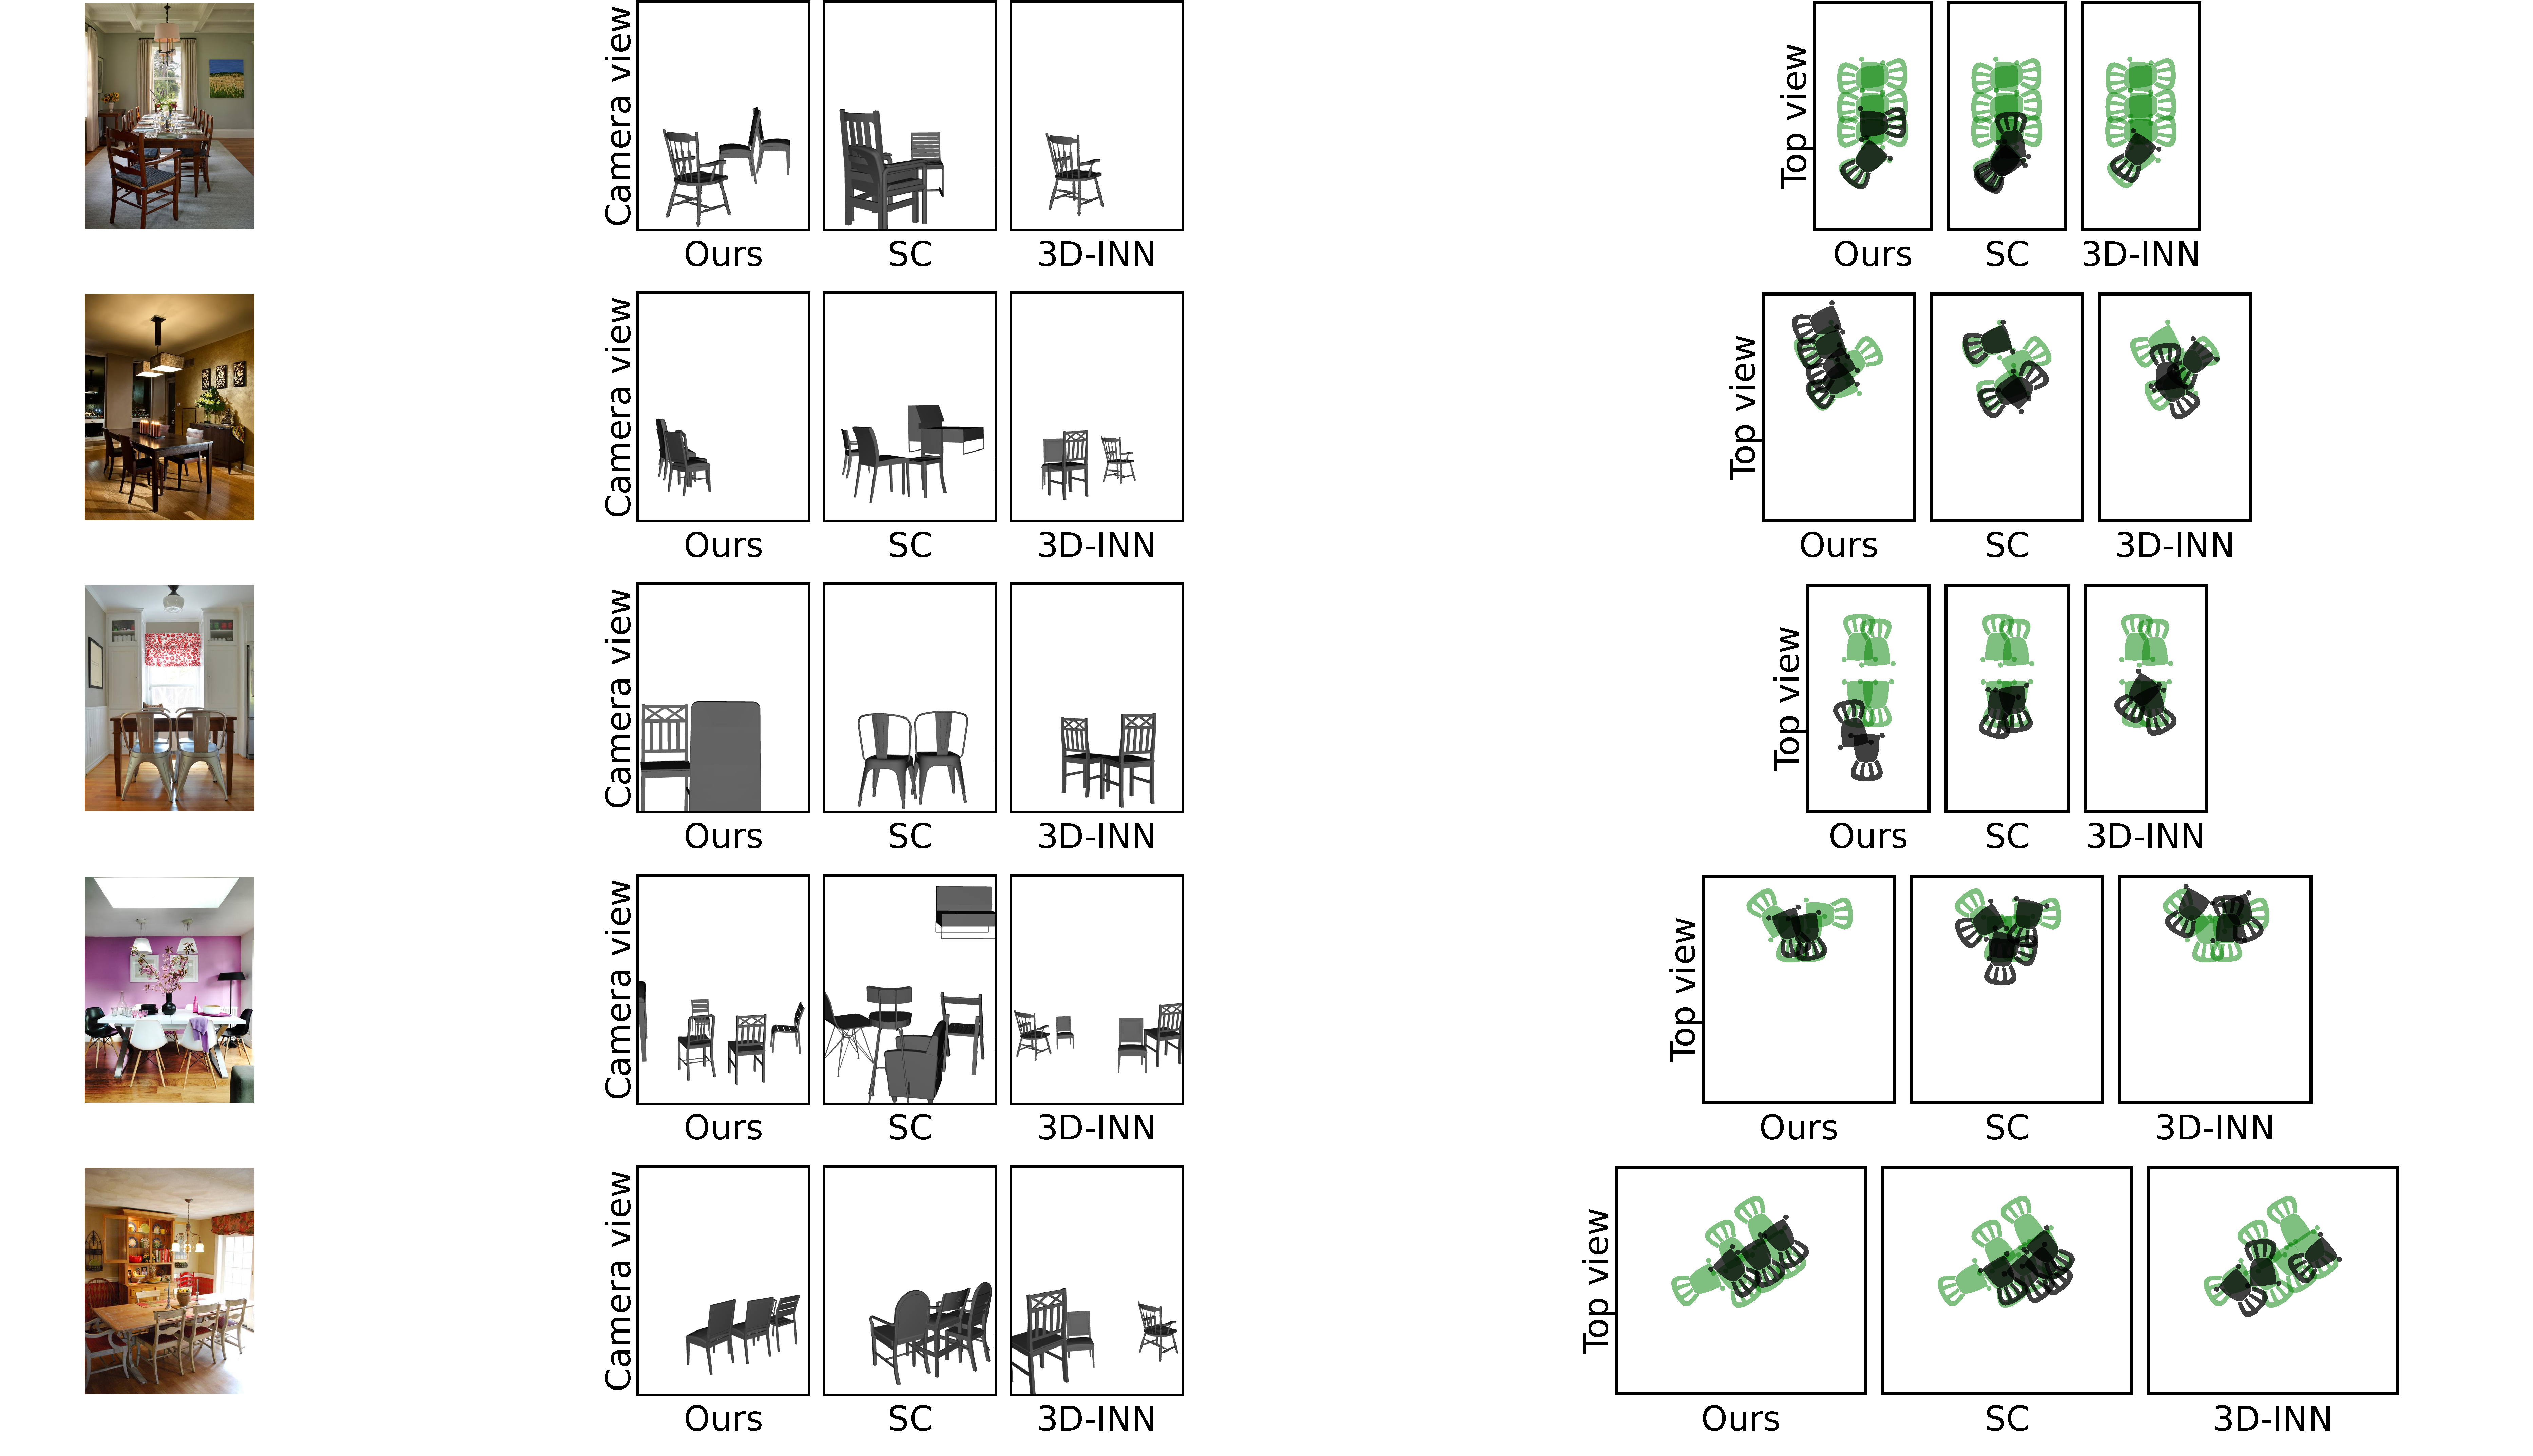
\includegraphics[width=\textwidth]{figures/qualitative_results/full/qual_results_0.pdf}
\end{sidewaysfigure}
\begin{sidewaysfigure}
    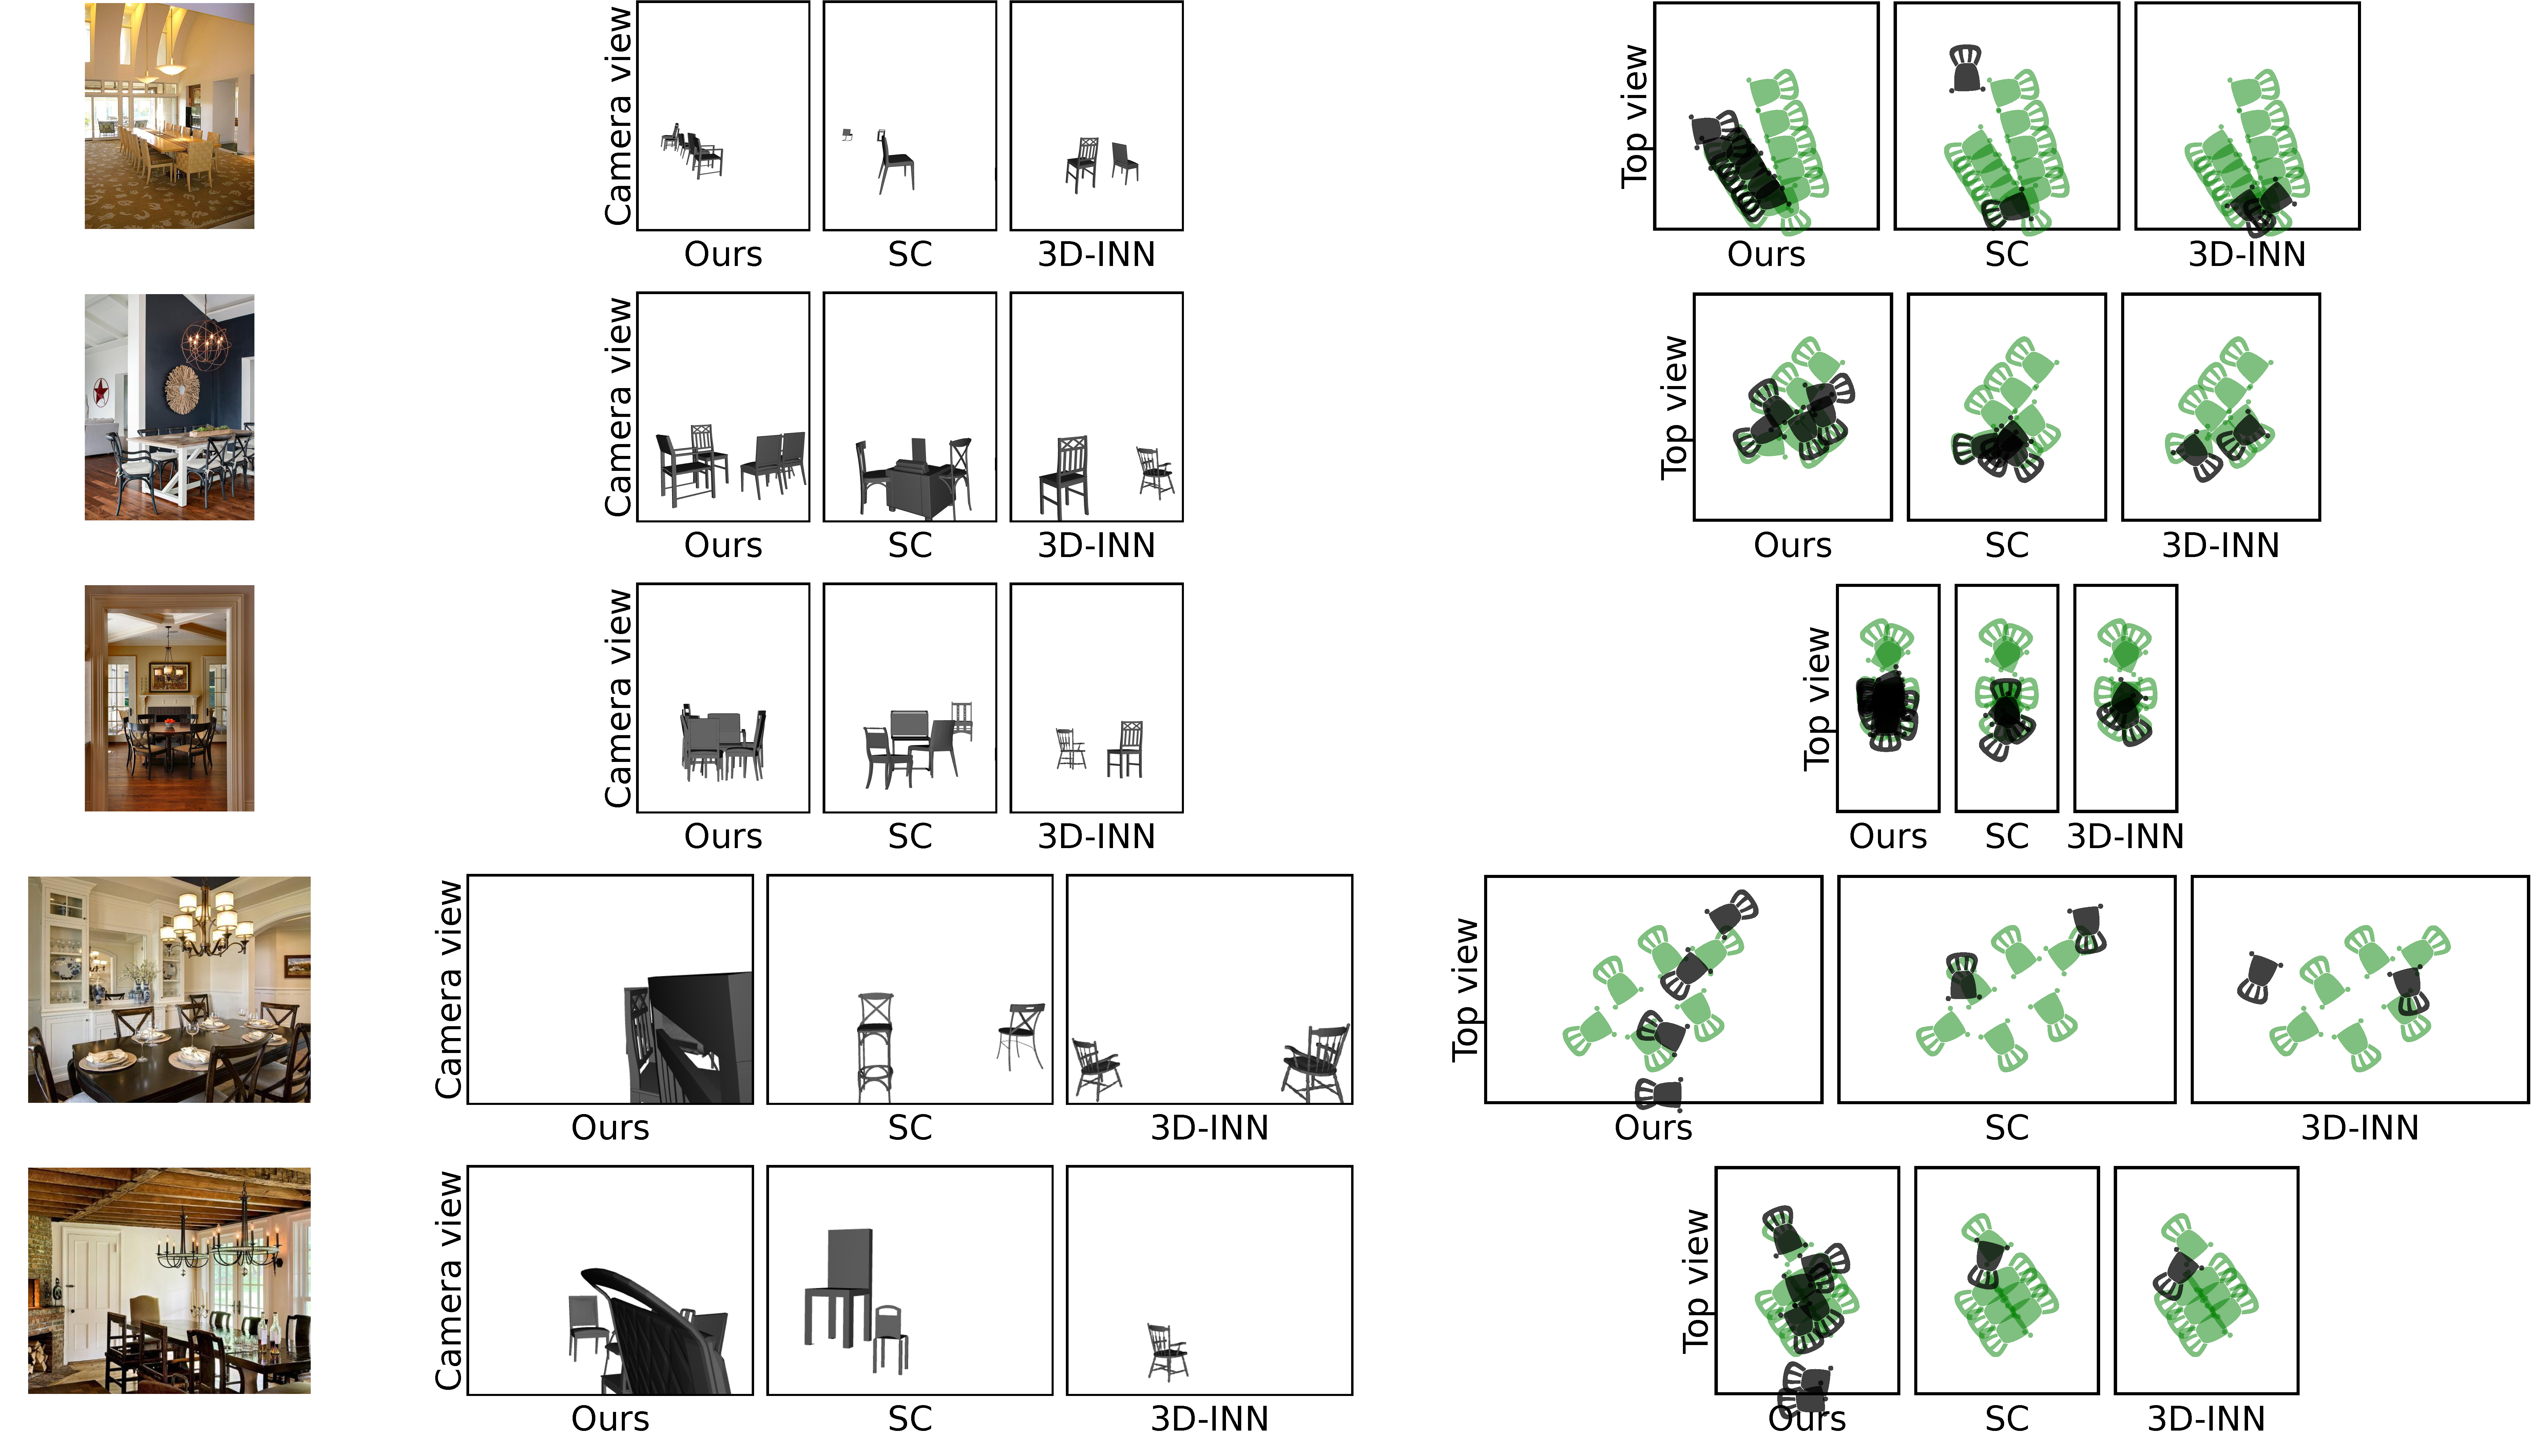
\includegraphics[width=\textwidth]{figures/qualitative_results/full/qual_results_1.pdf}
\end{sidewaysfigure}
\begin{sidewaysfigure}
    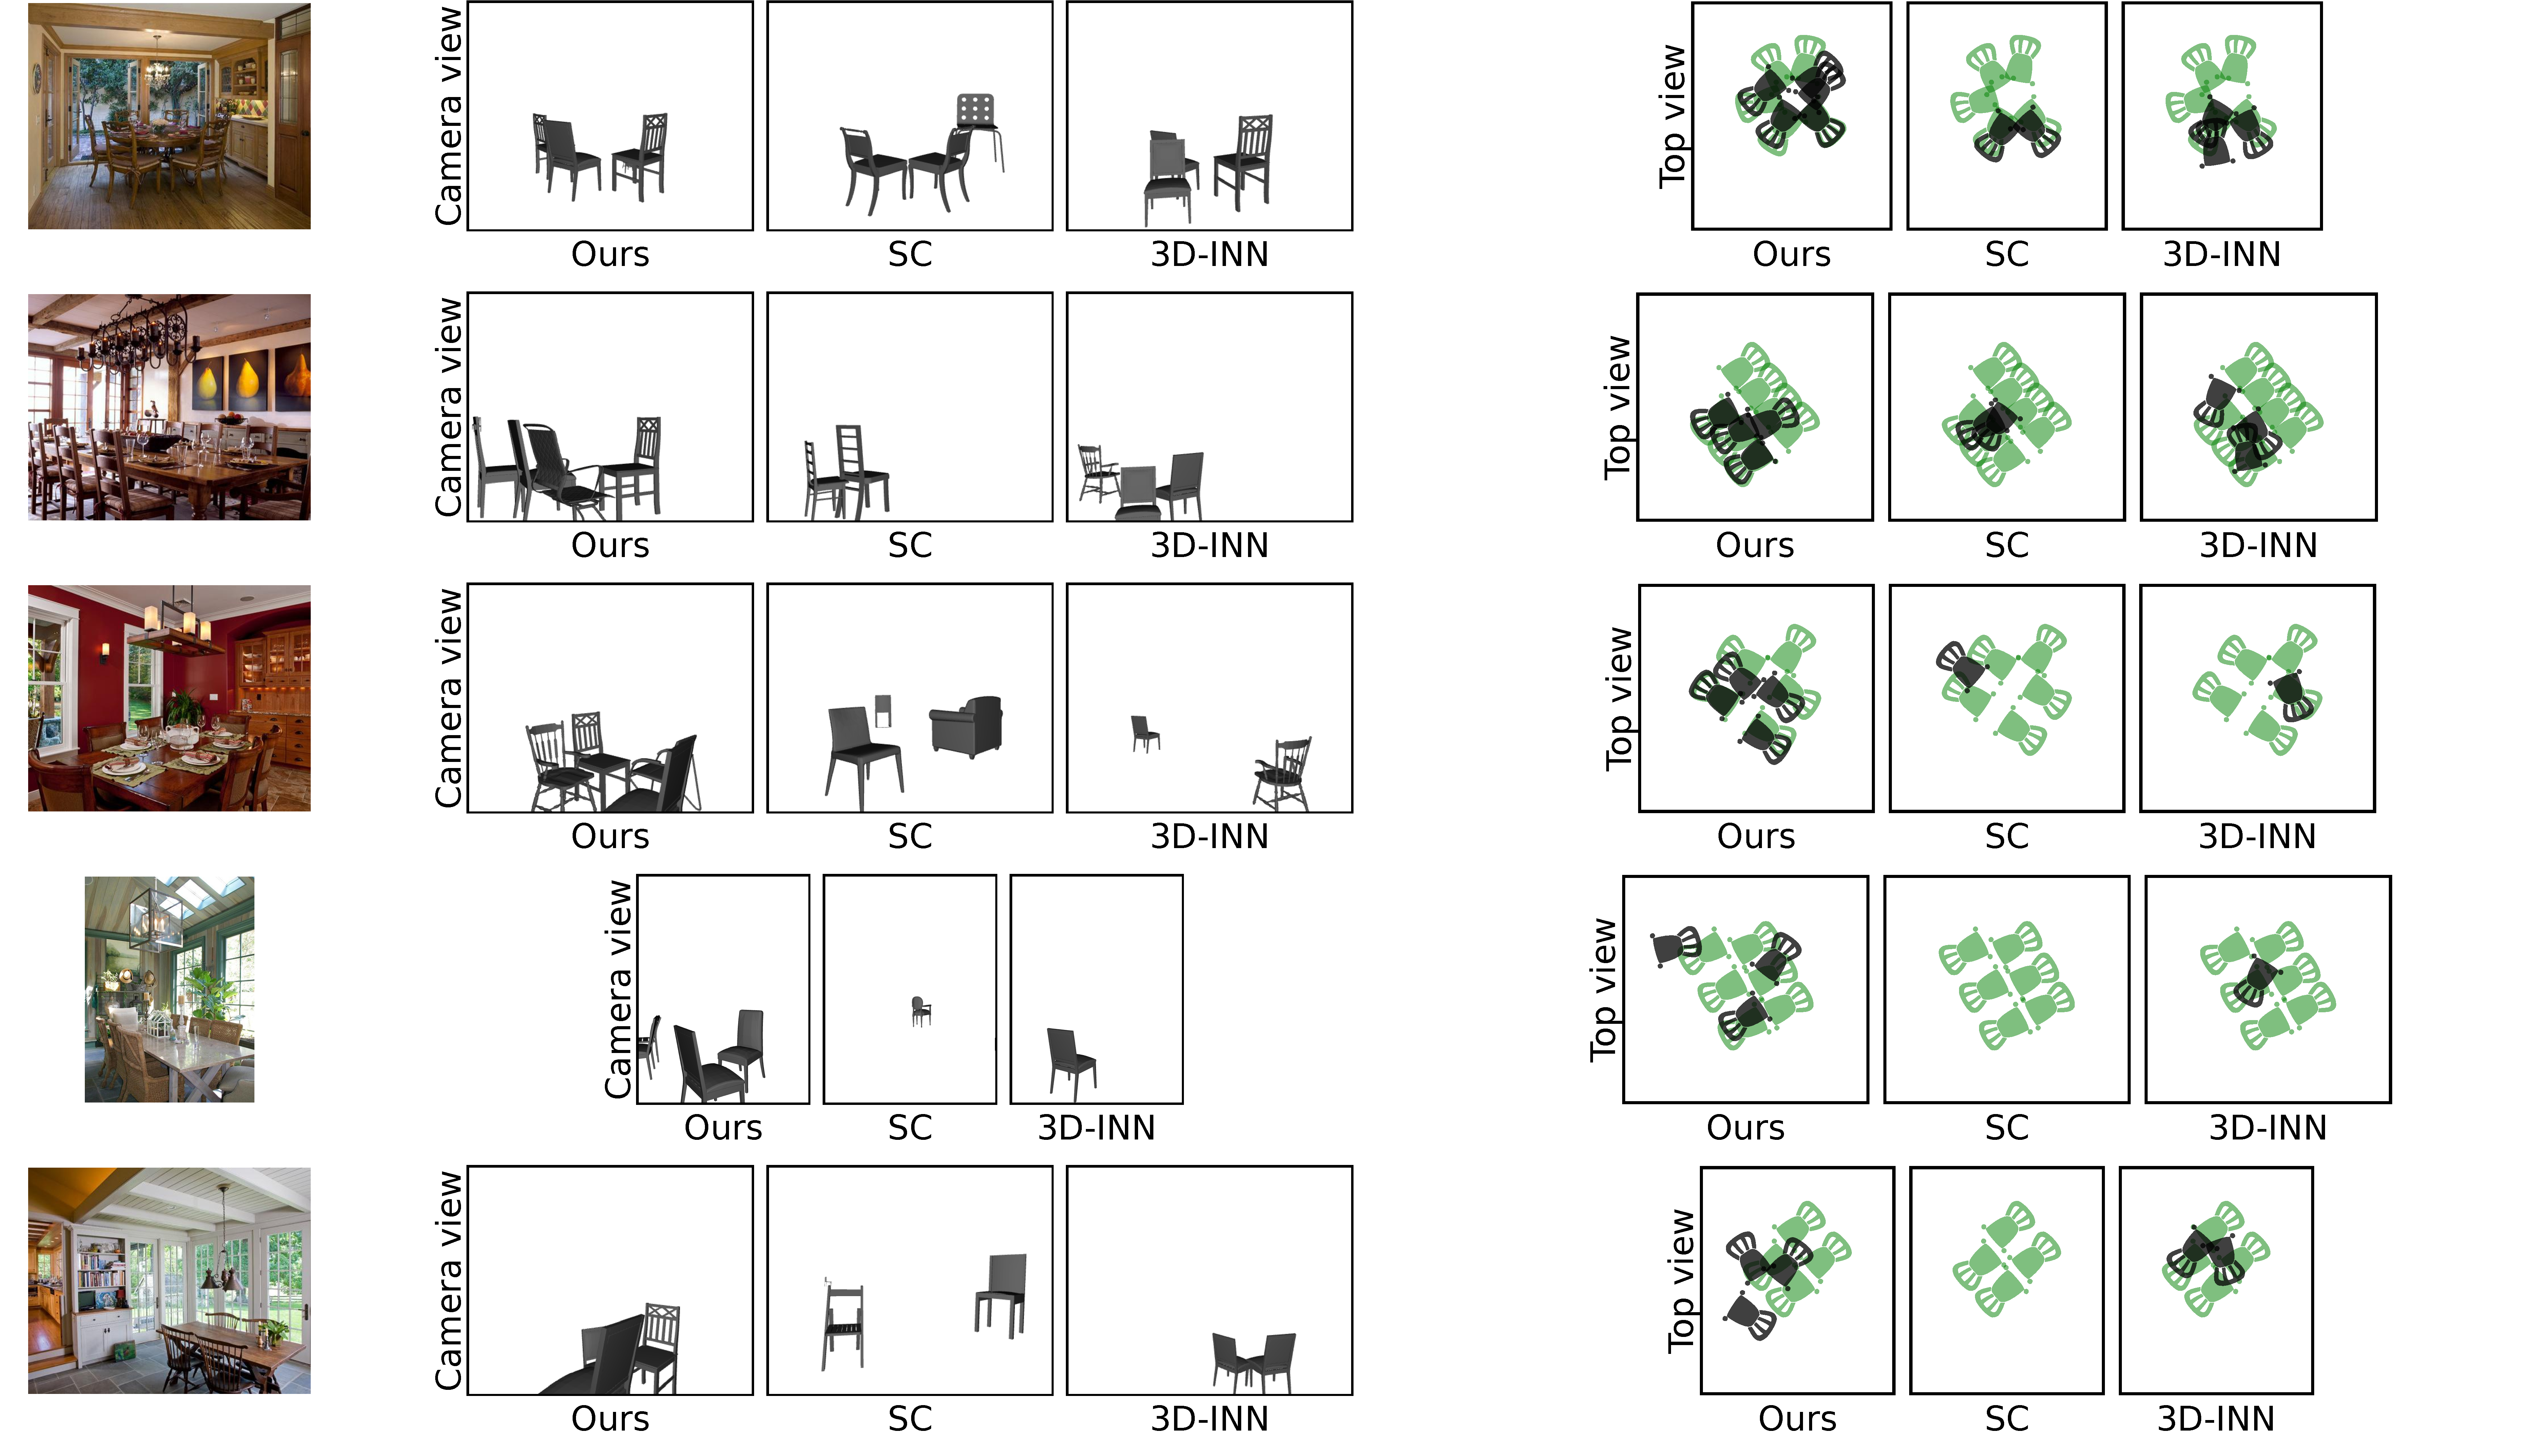
\includegraphics[width=\textwidth]{figures/qualitative_results/full/qual_results_2.pdf}
\end{sidewaysfigure}
\begin{sidewaysfigure}
    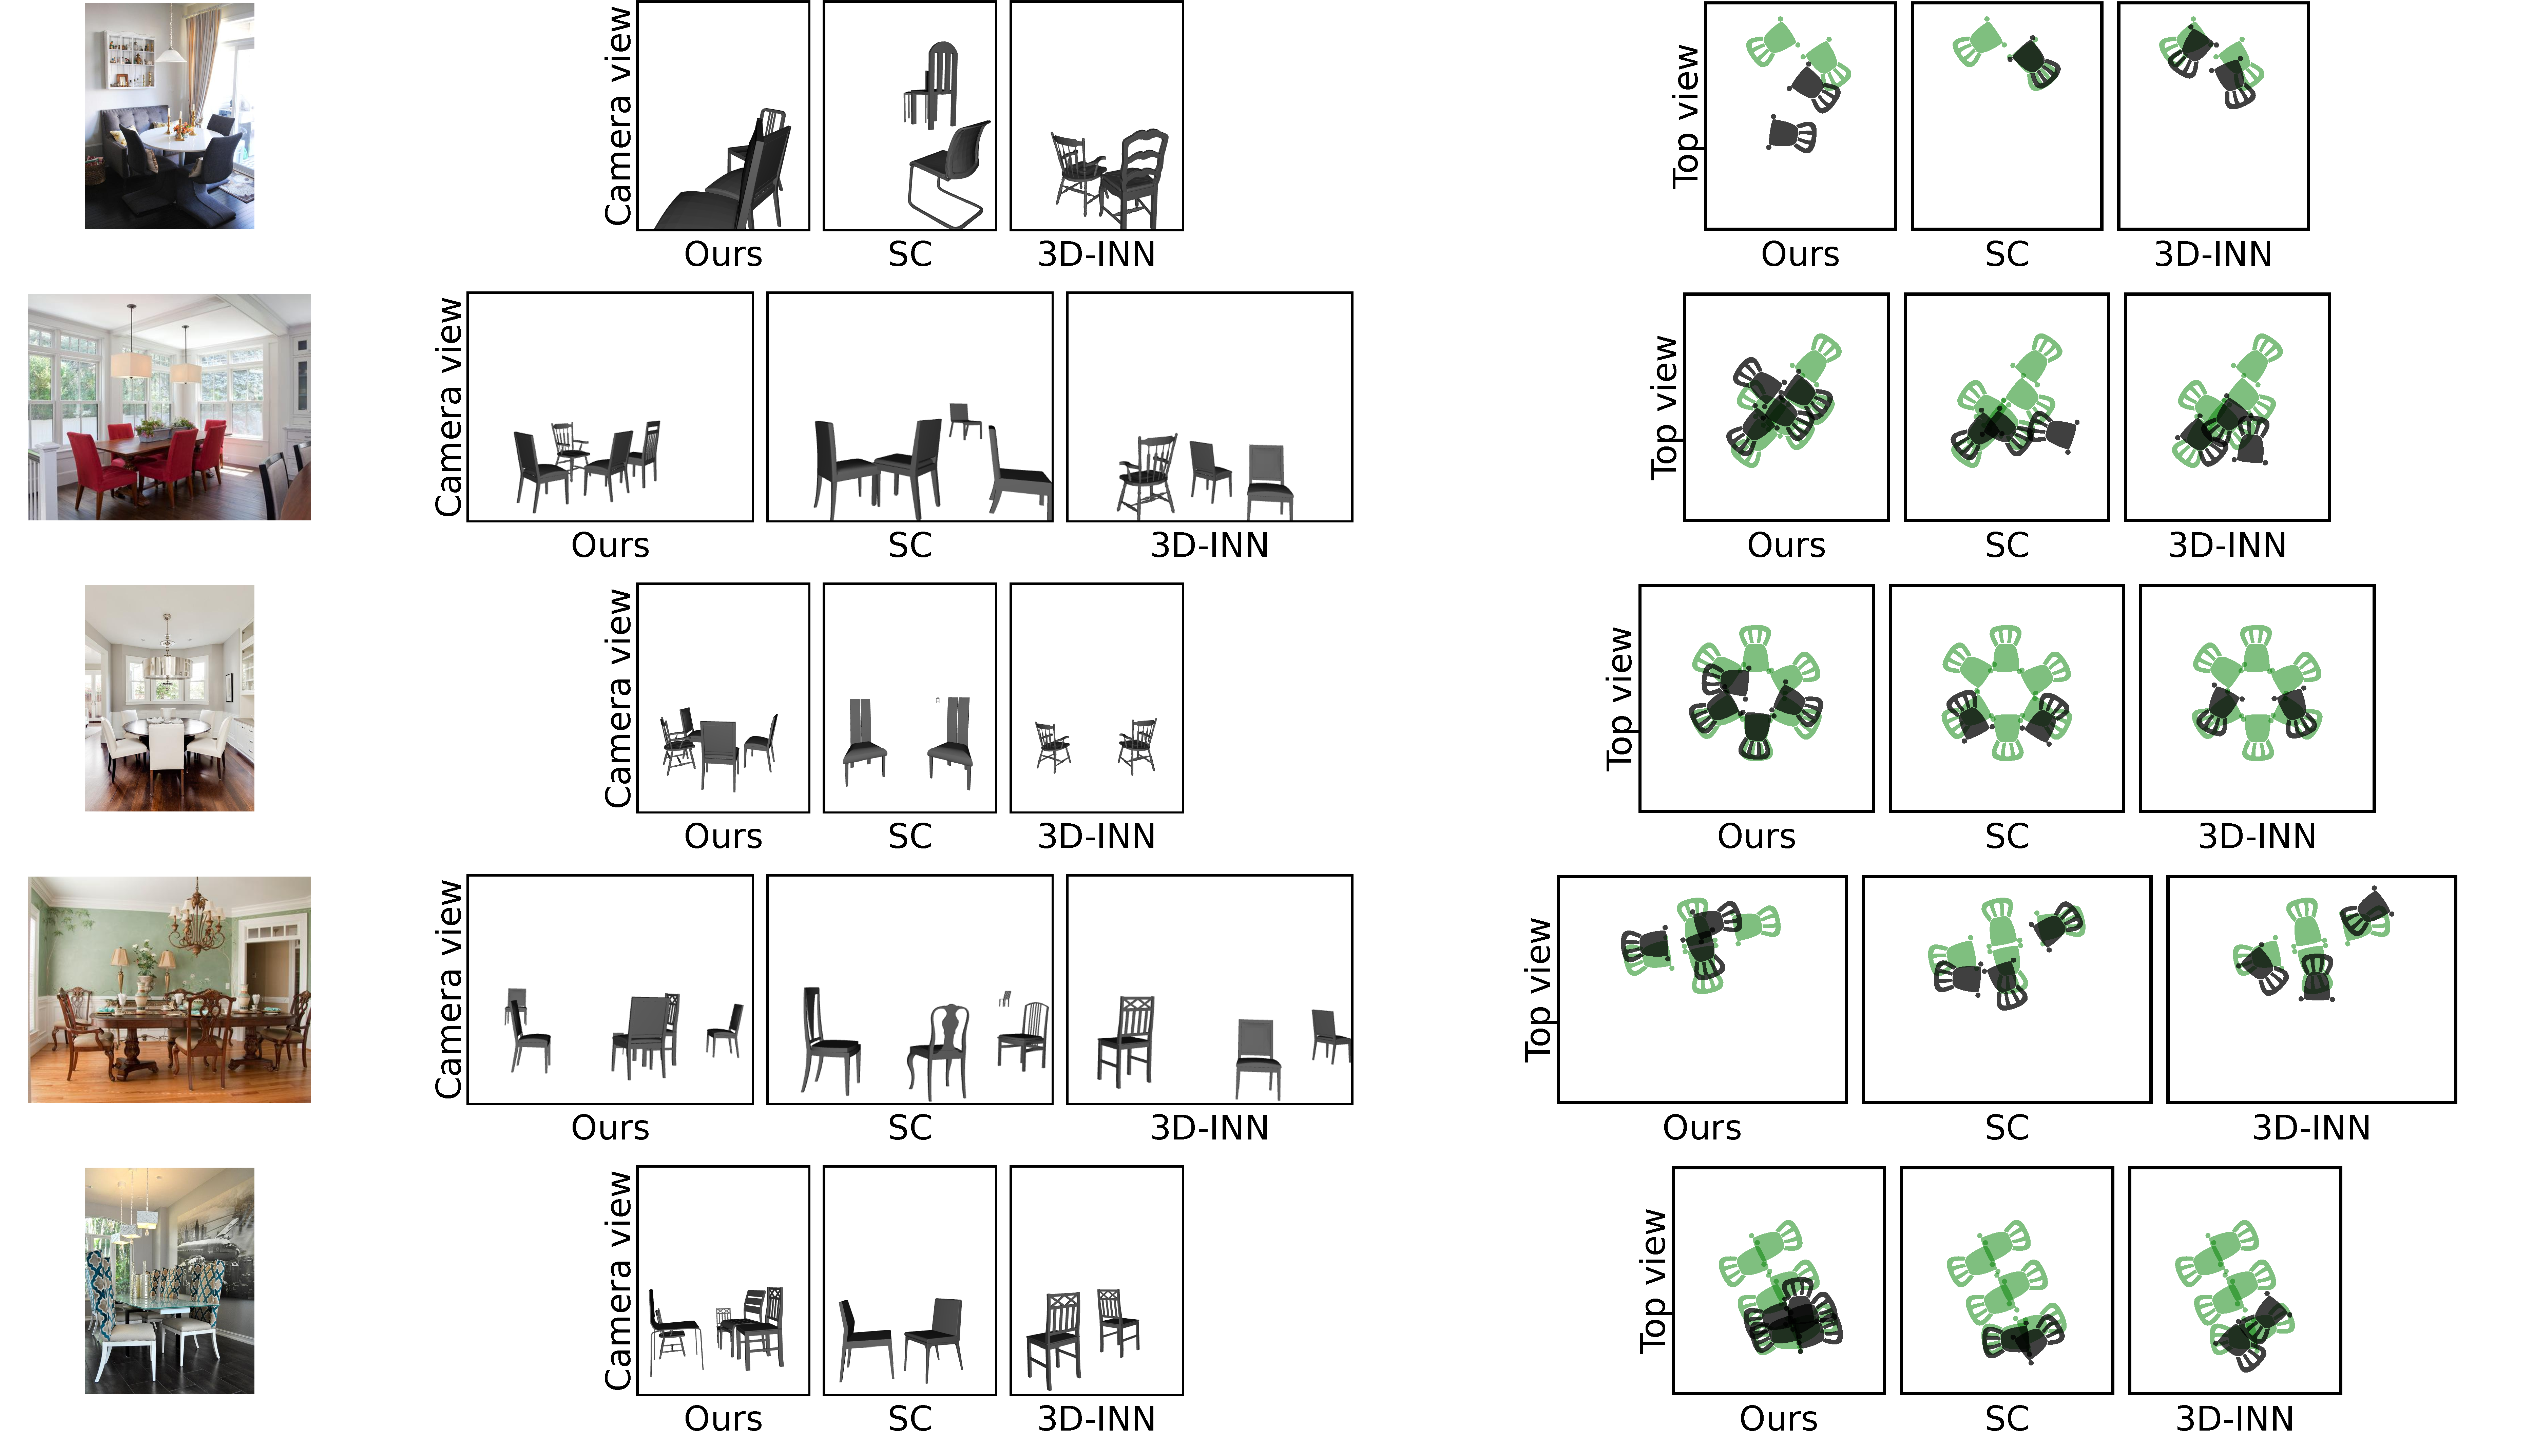
\includegraphics[width=\textwidth]{figures/qualitative_results/full/qual_results_3.pdf}
\end{sidewaysfigure}
\begin{sidewaysfigure}
    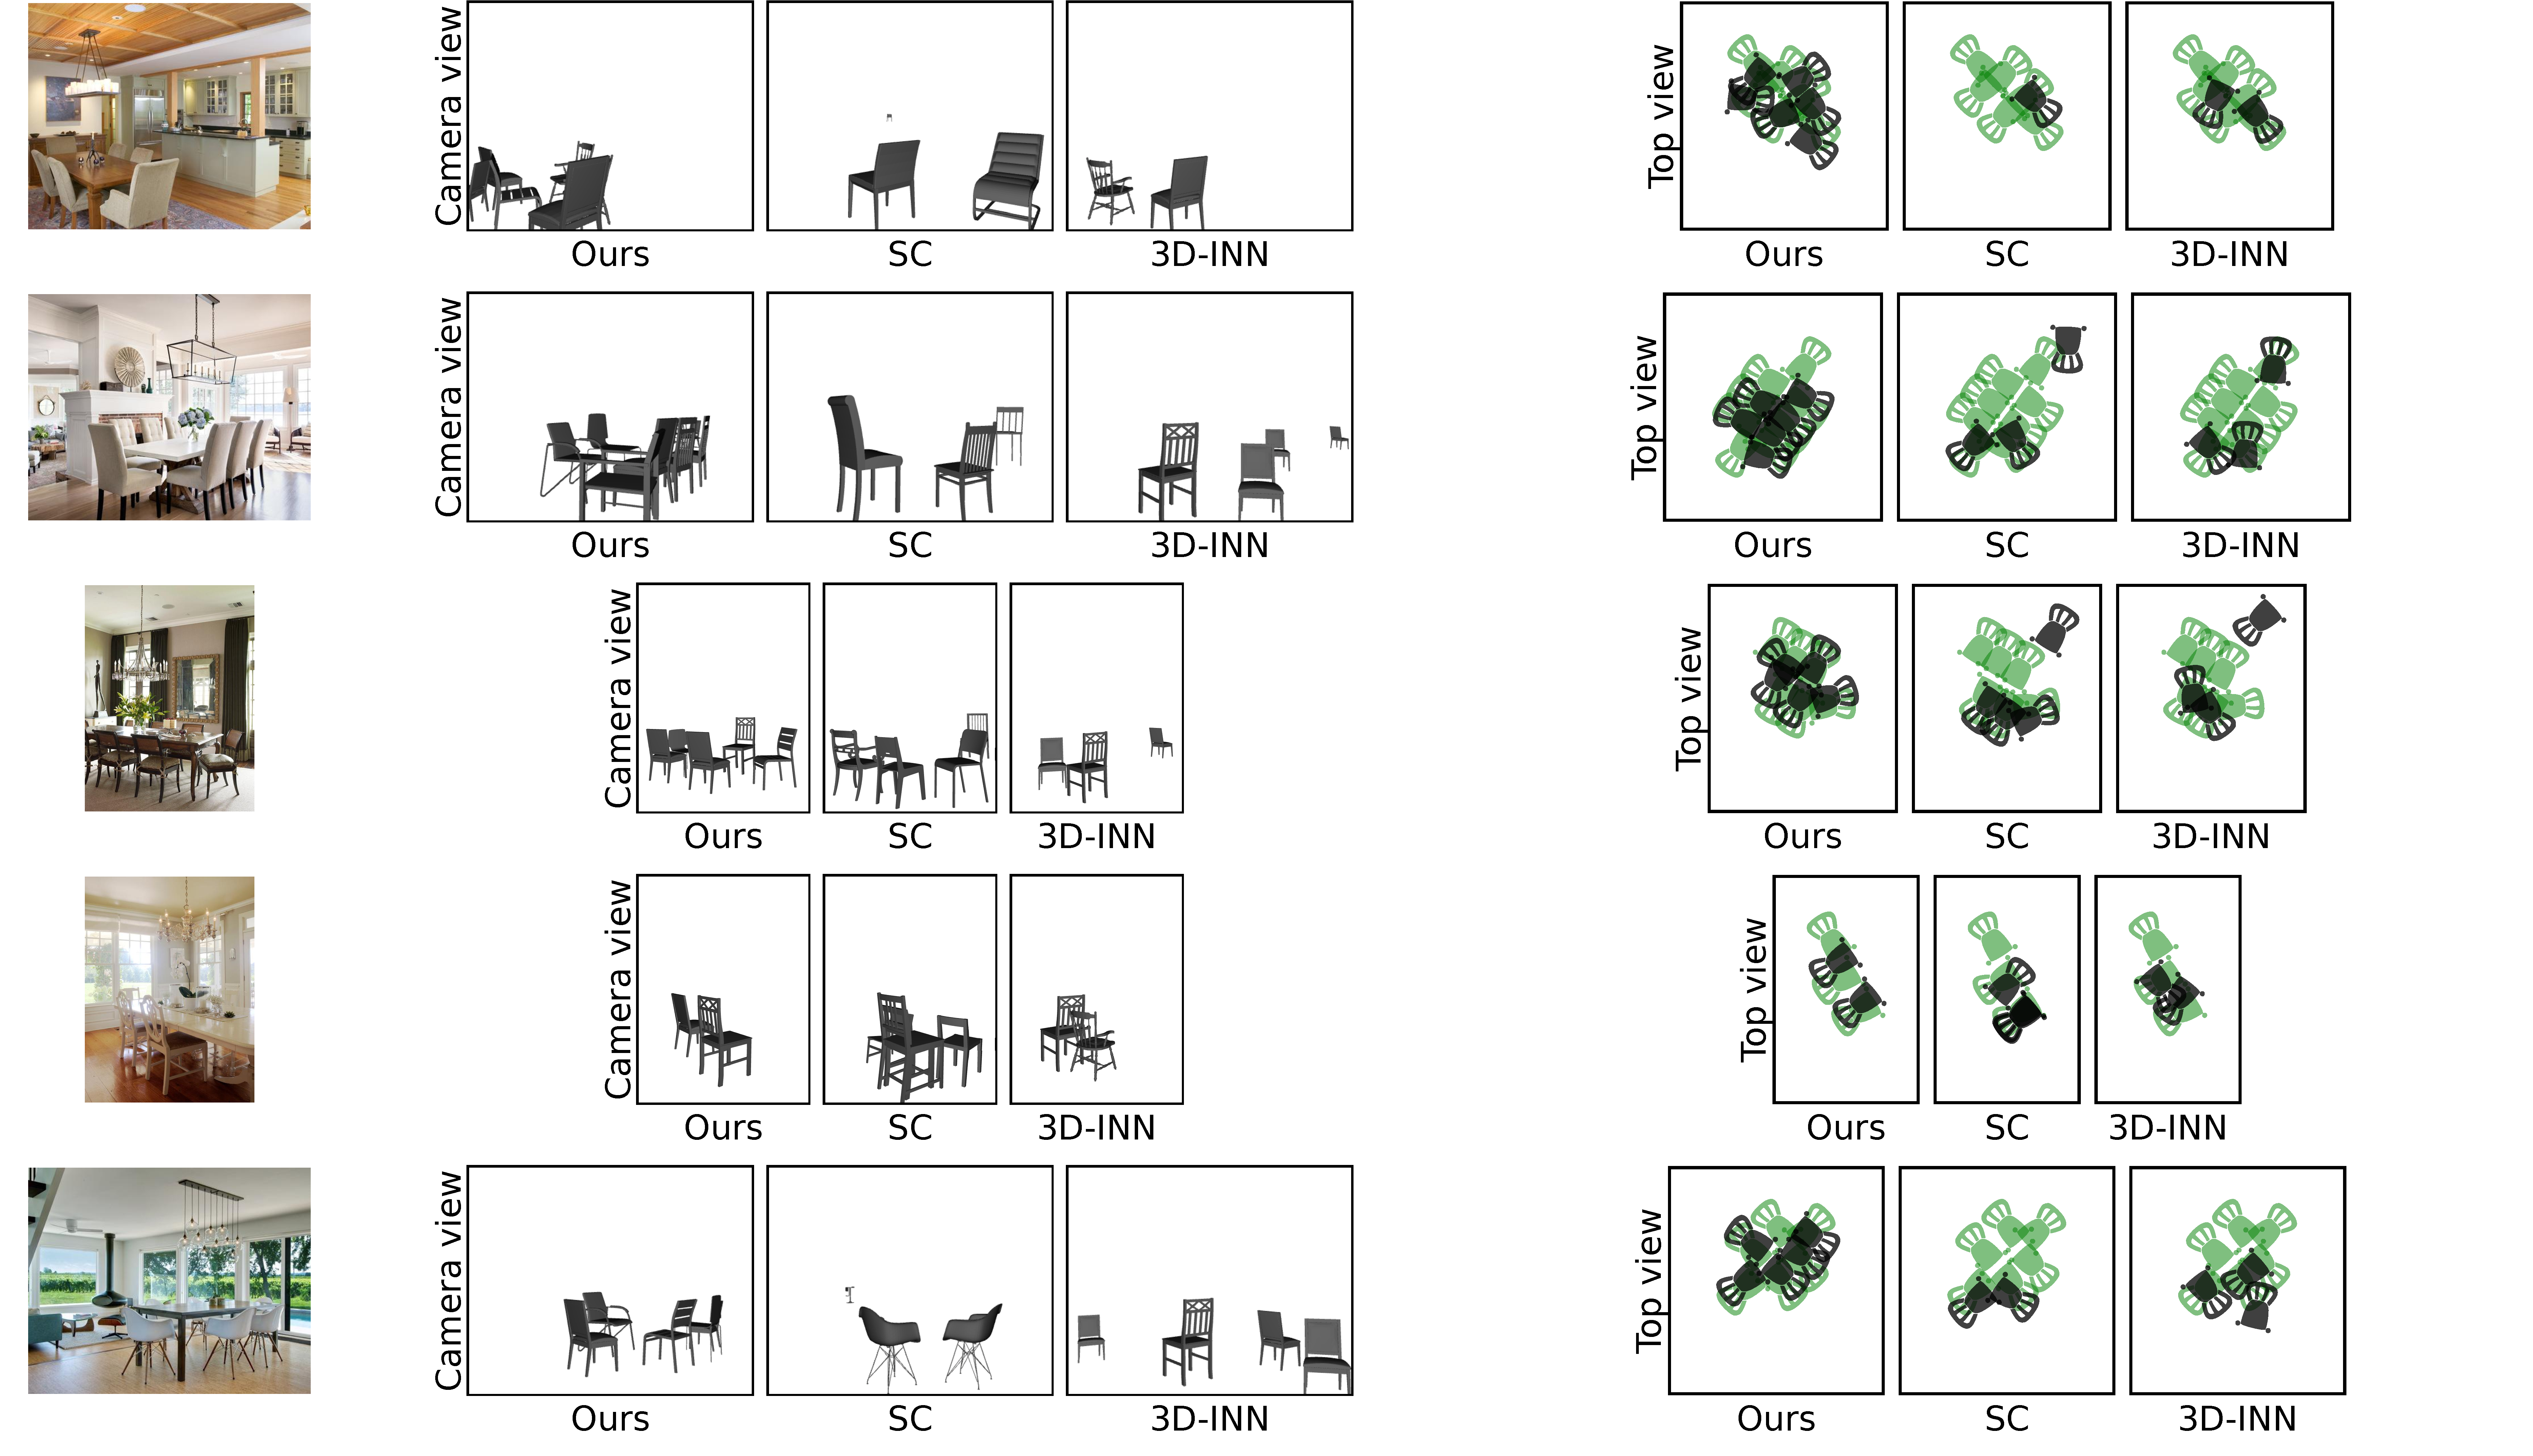
\includegraphics[width=\textwidth]{figures/qualitative_results/full/qual_results_4.pdf}
\end{sidewaysfigure}
\begin{sidewaysfigure}
    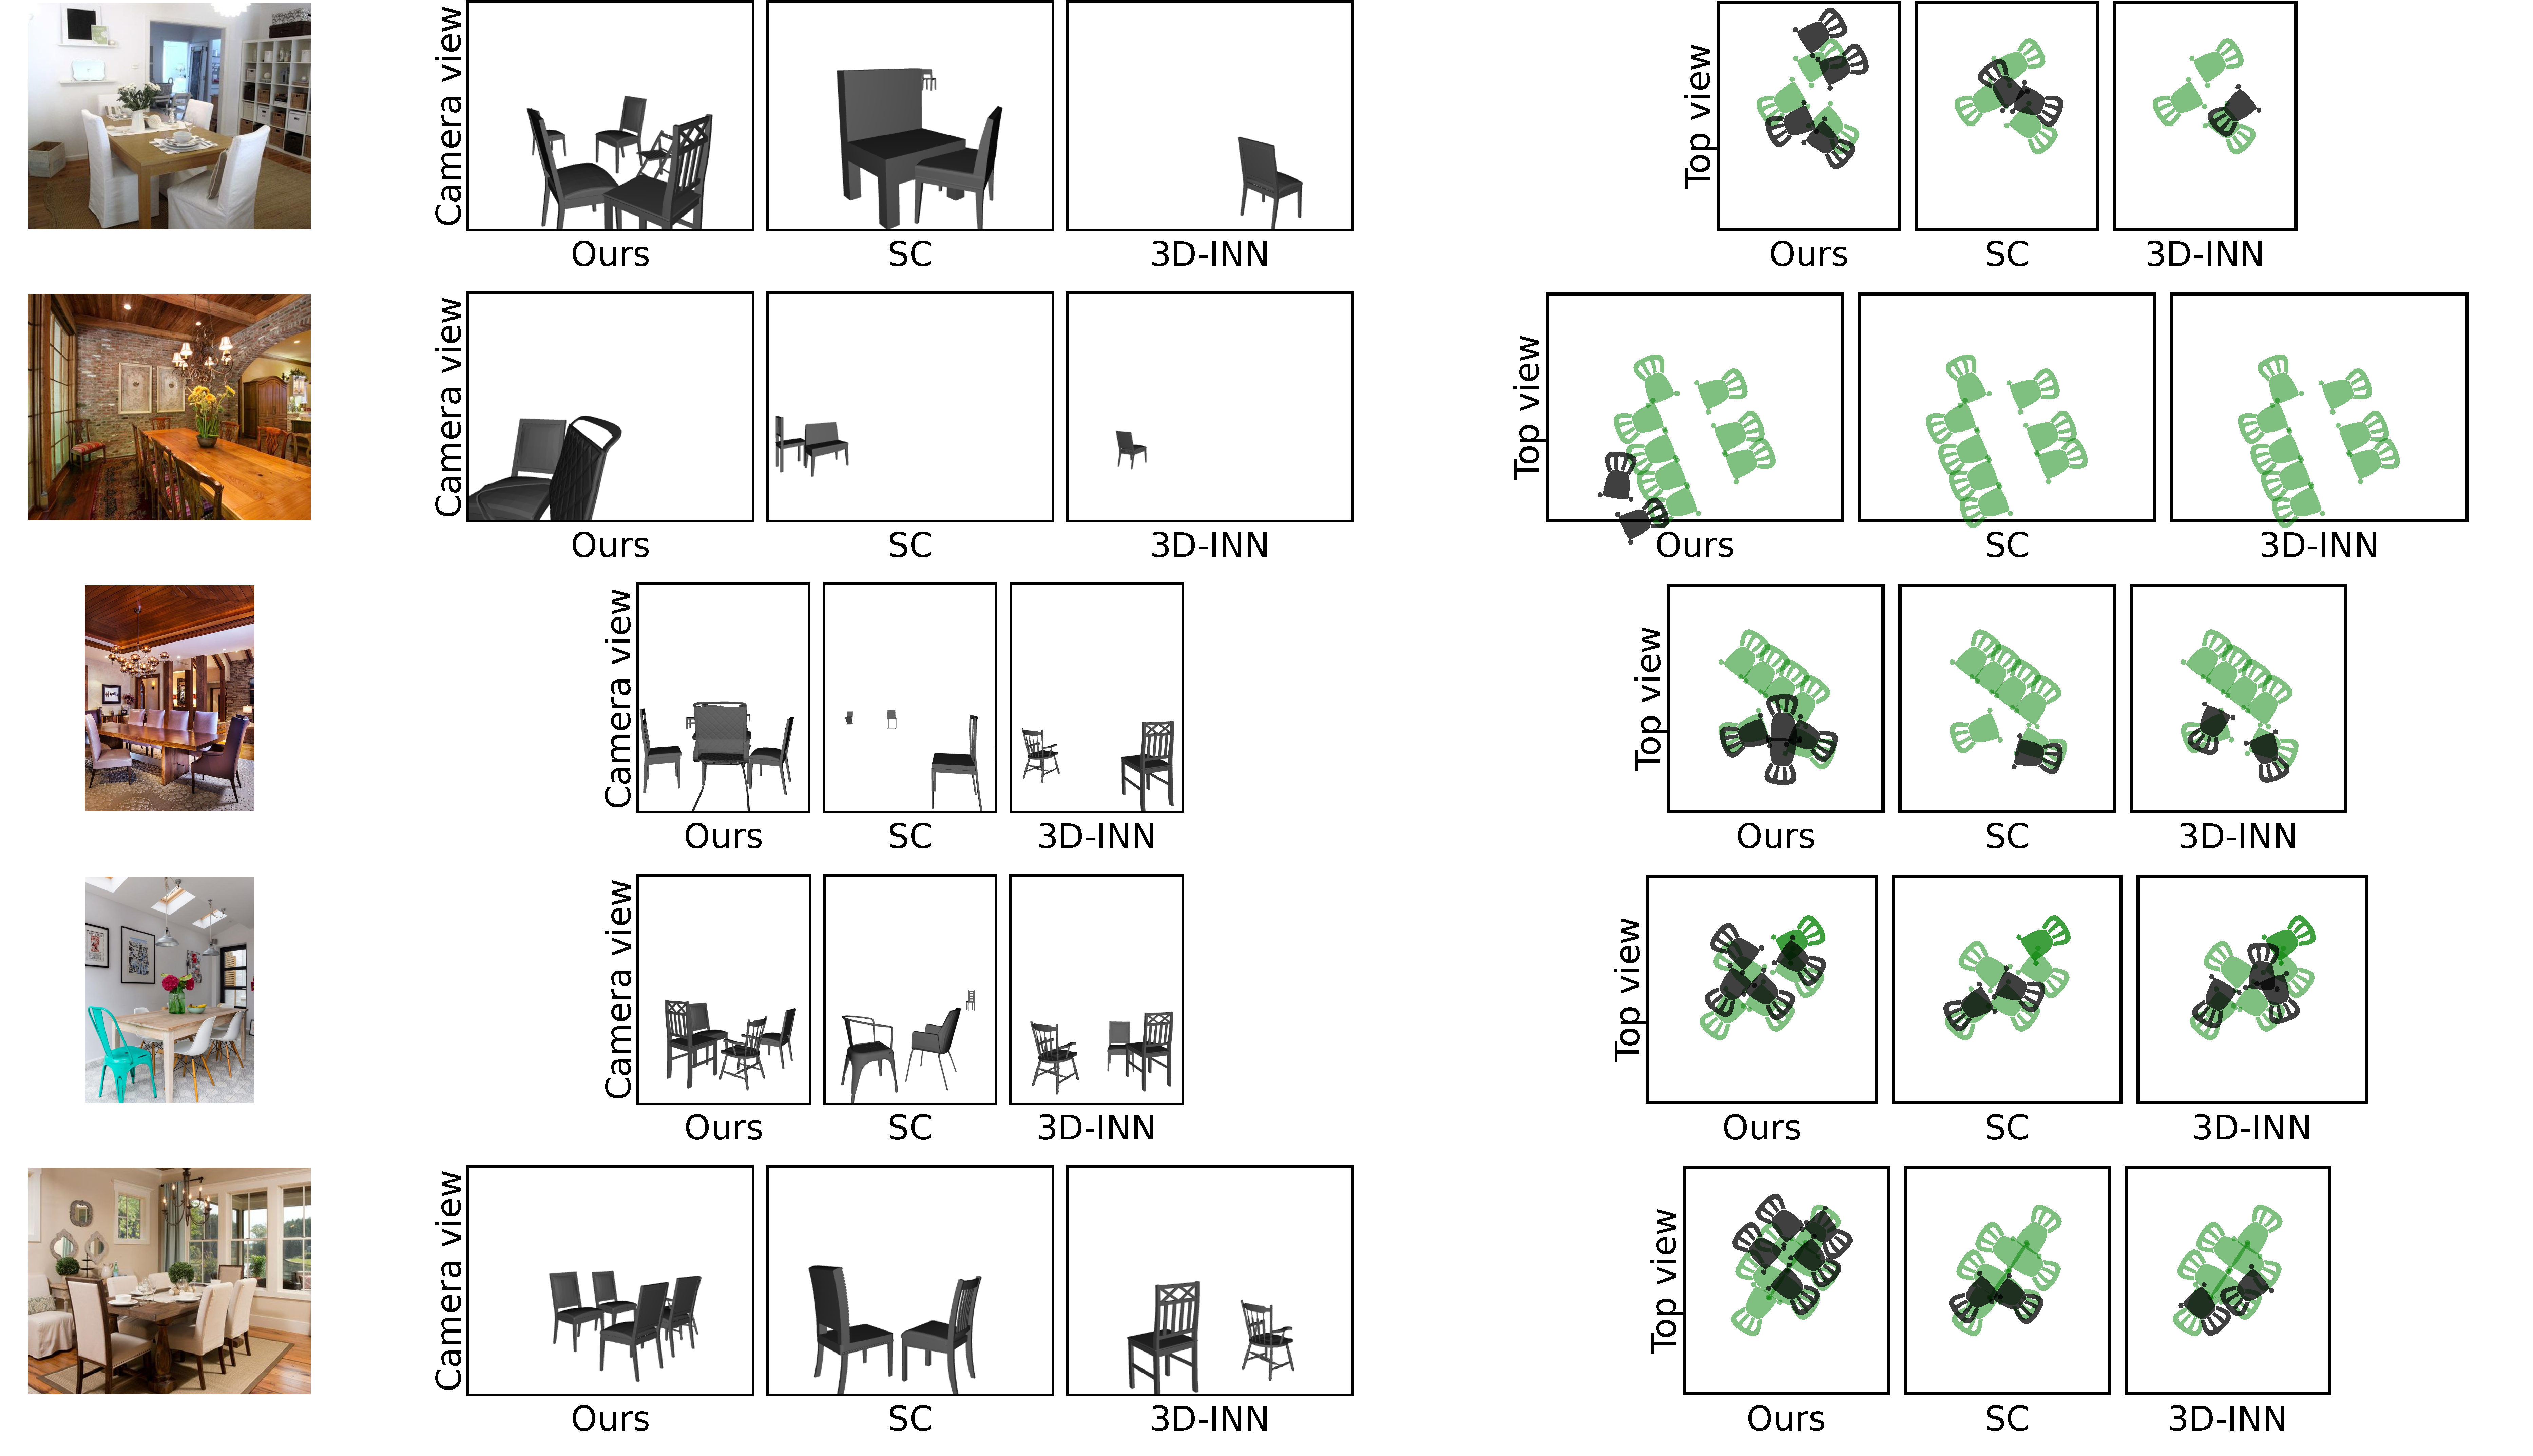
\includegraphics[width=\textwidth]{figures/qualitative_results/full/qual_results_5.pdf}
\end{sidewaysfigure}
\begin{sidewaysfigure}
    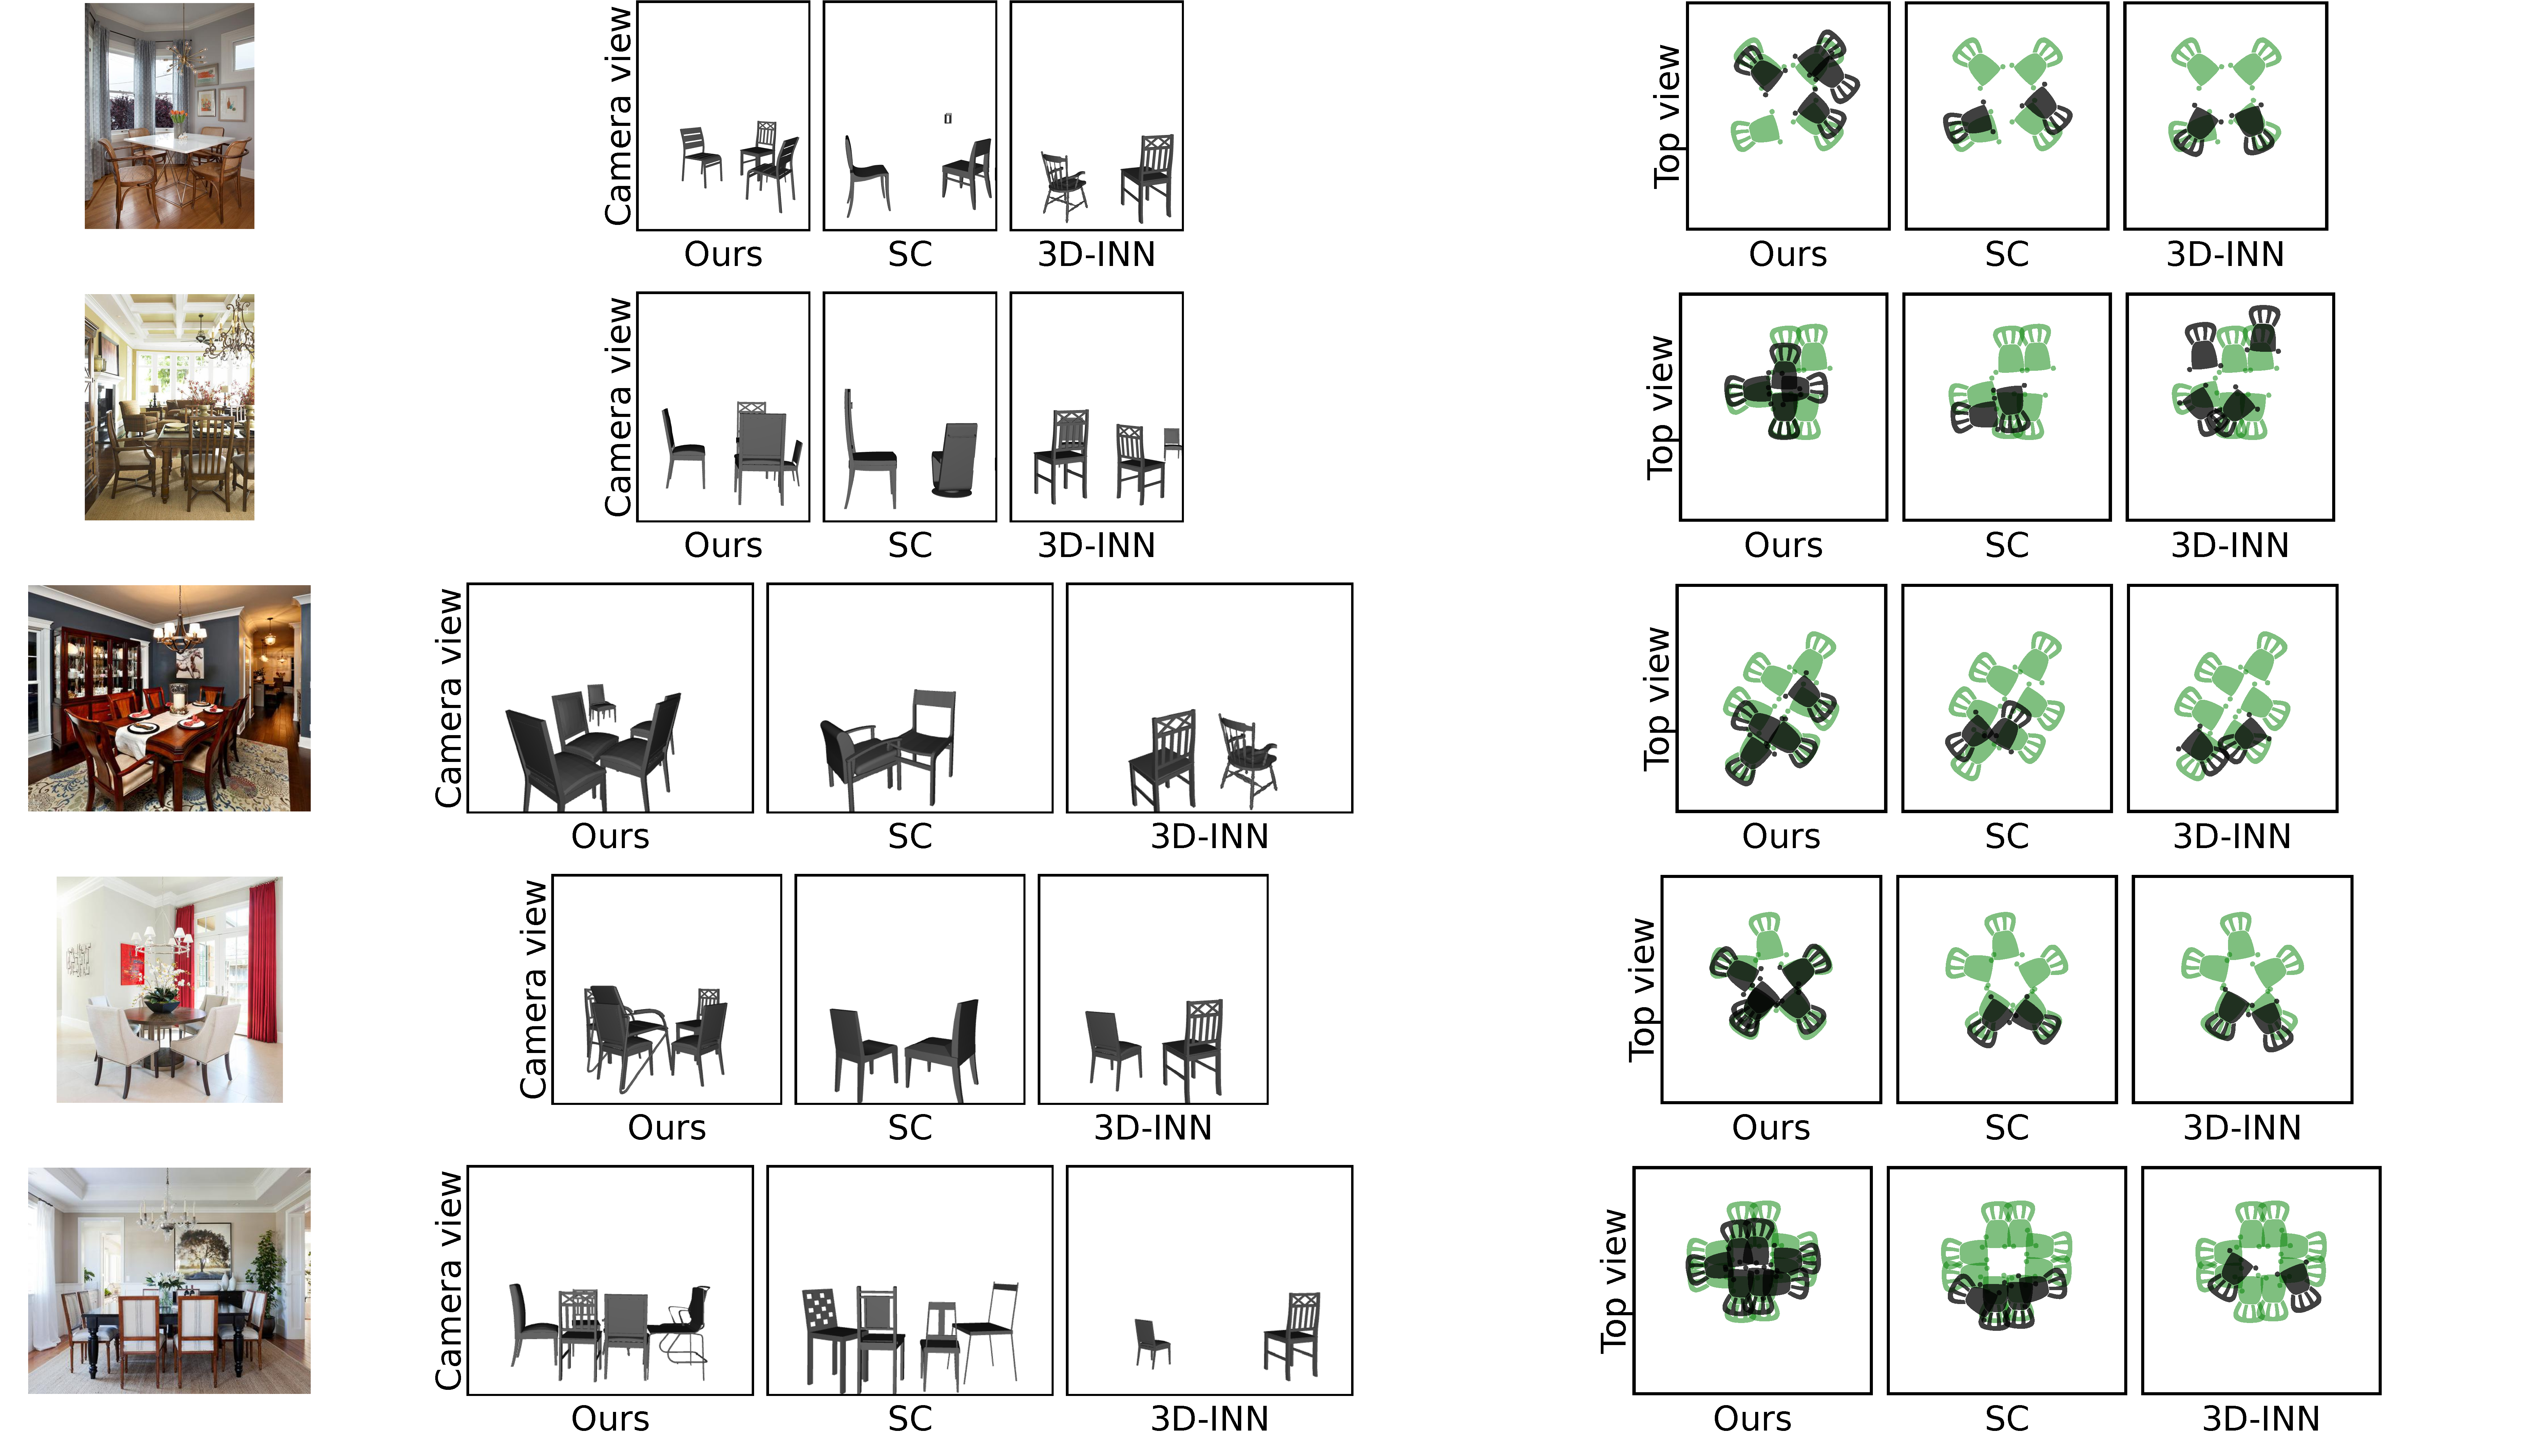
\includegraphics[width=\textwidth]{figures/qualitative_results/full/qual_results_6.pdf}
\end{sidewaysfigure}
\begin{sidewaysfigure}
    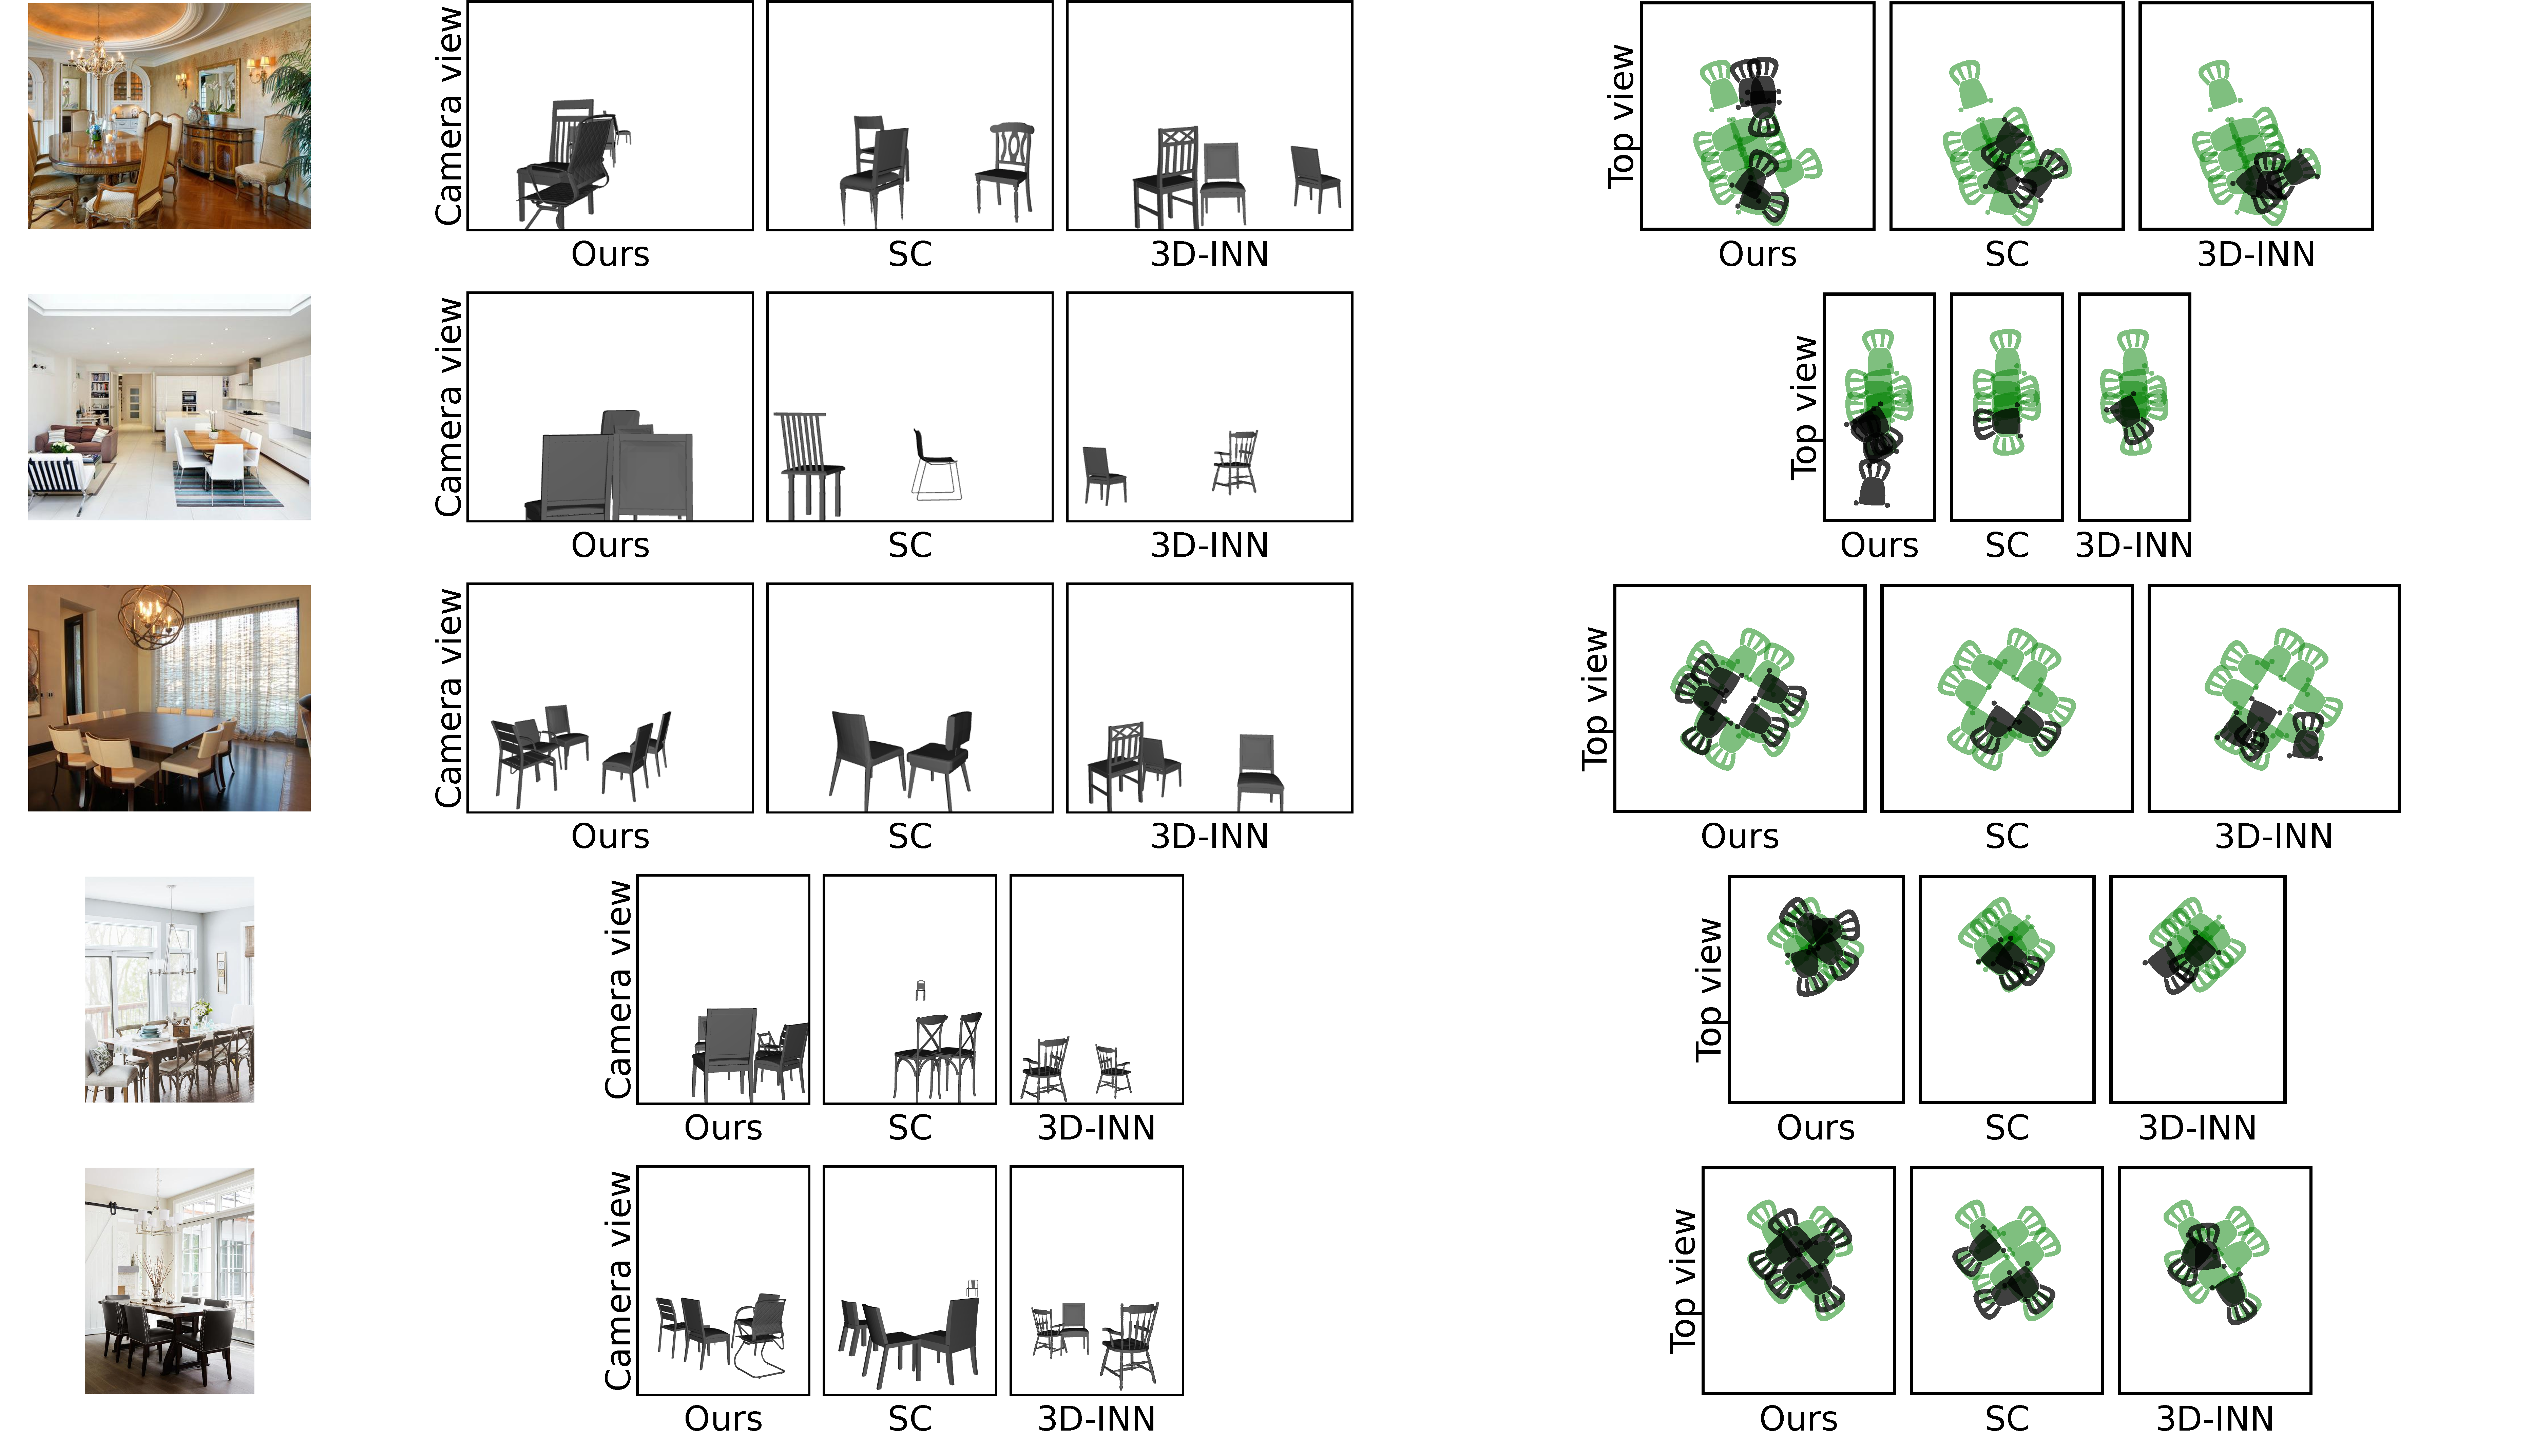
\includegraphics[width=\textwidth]{figures/qualitative_results/full/qual_results_7.pdf}
\end{sidewaysfigure}
\begin{sidewaysfigure}
    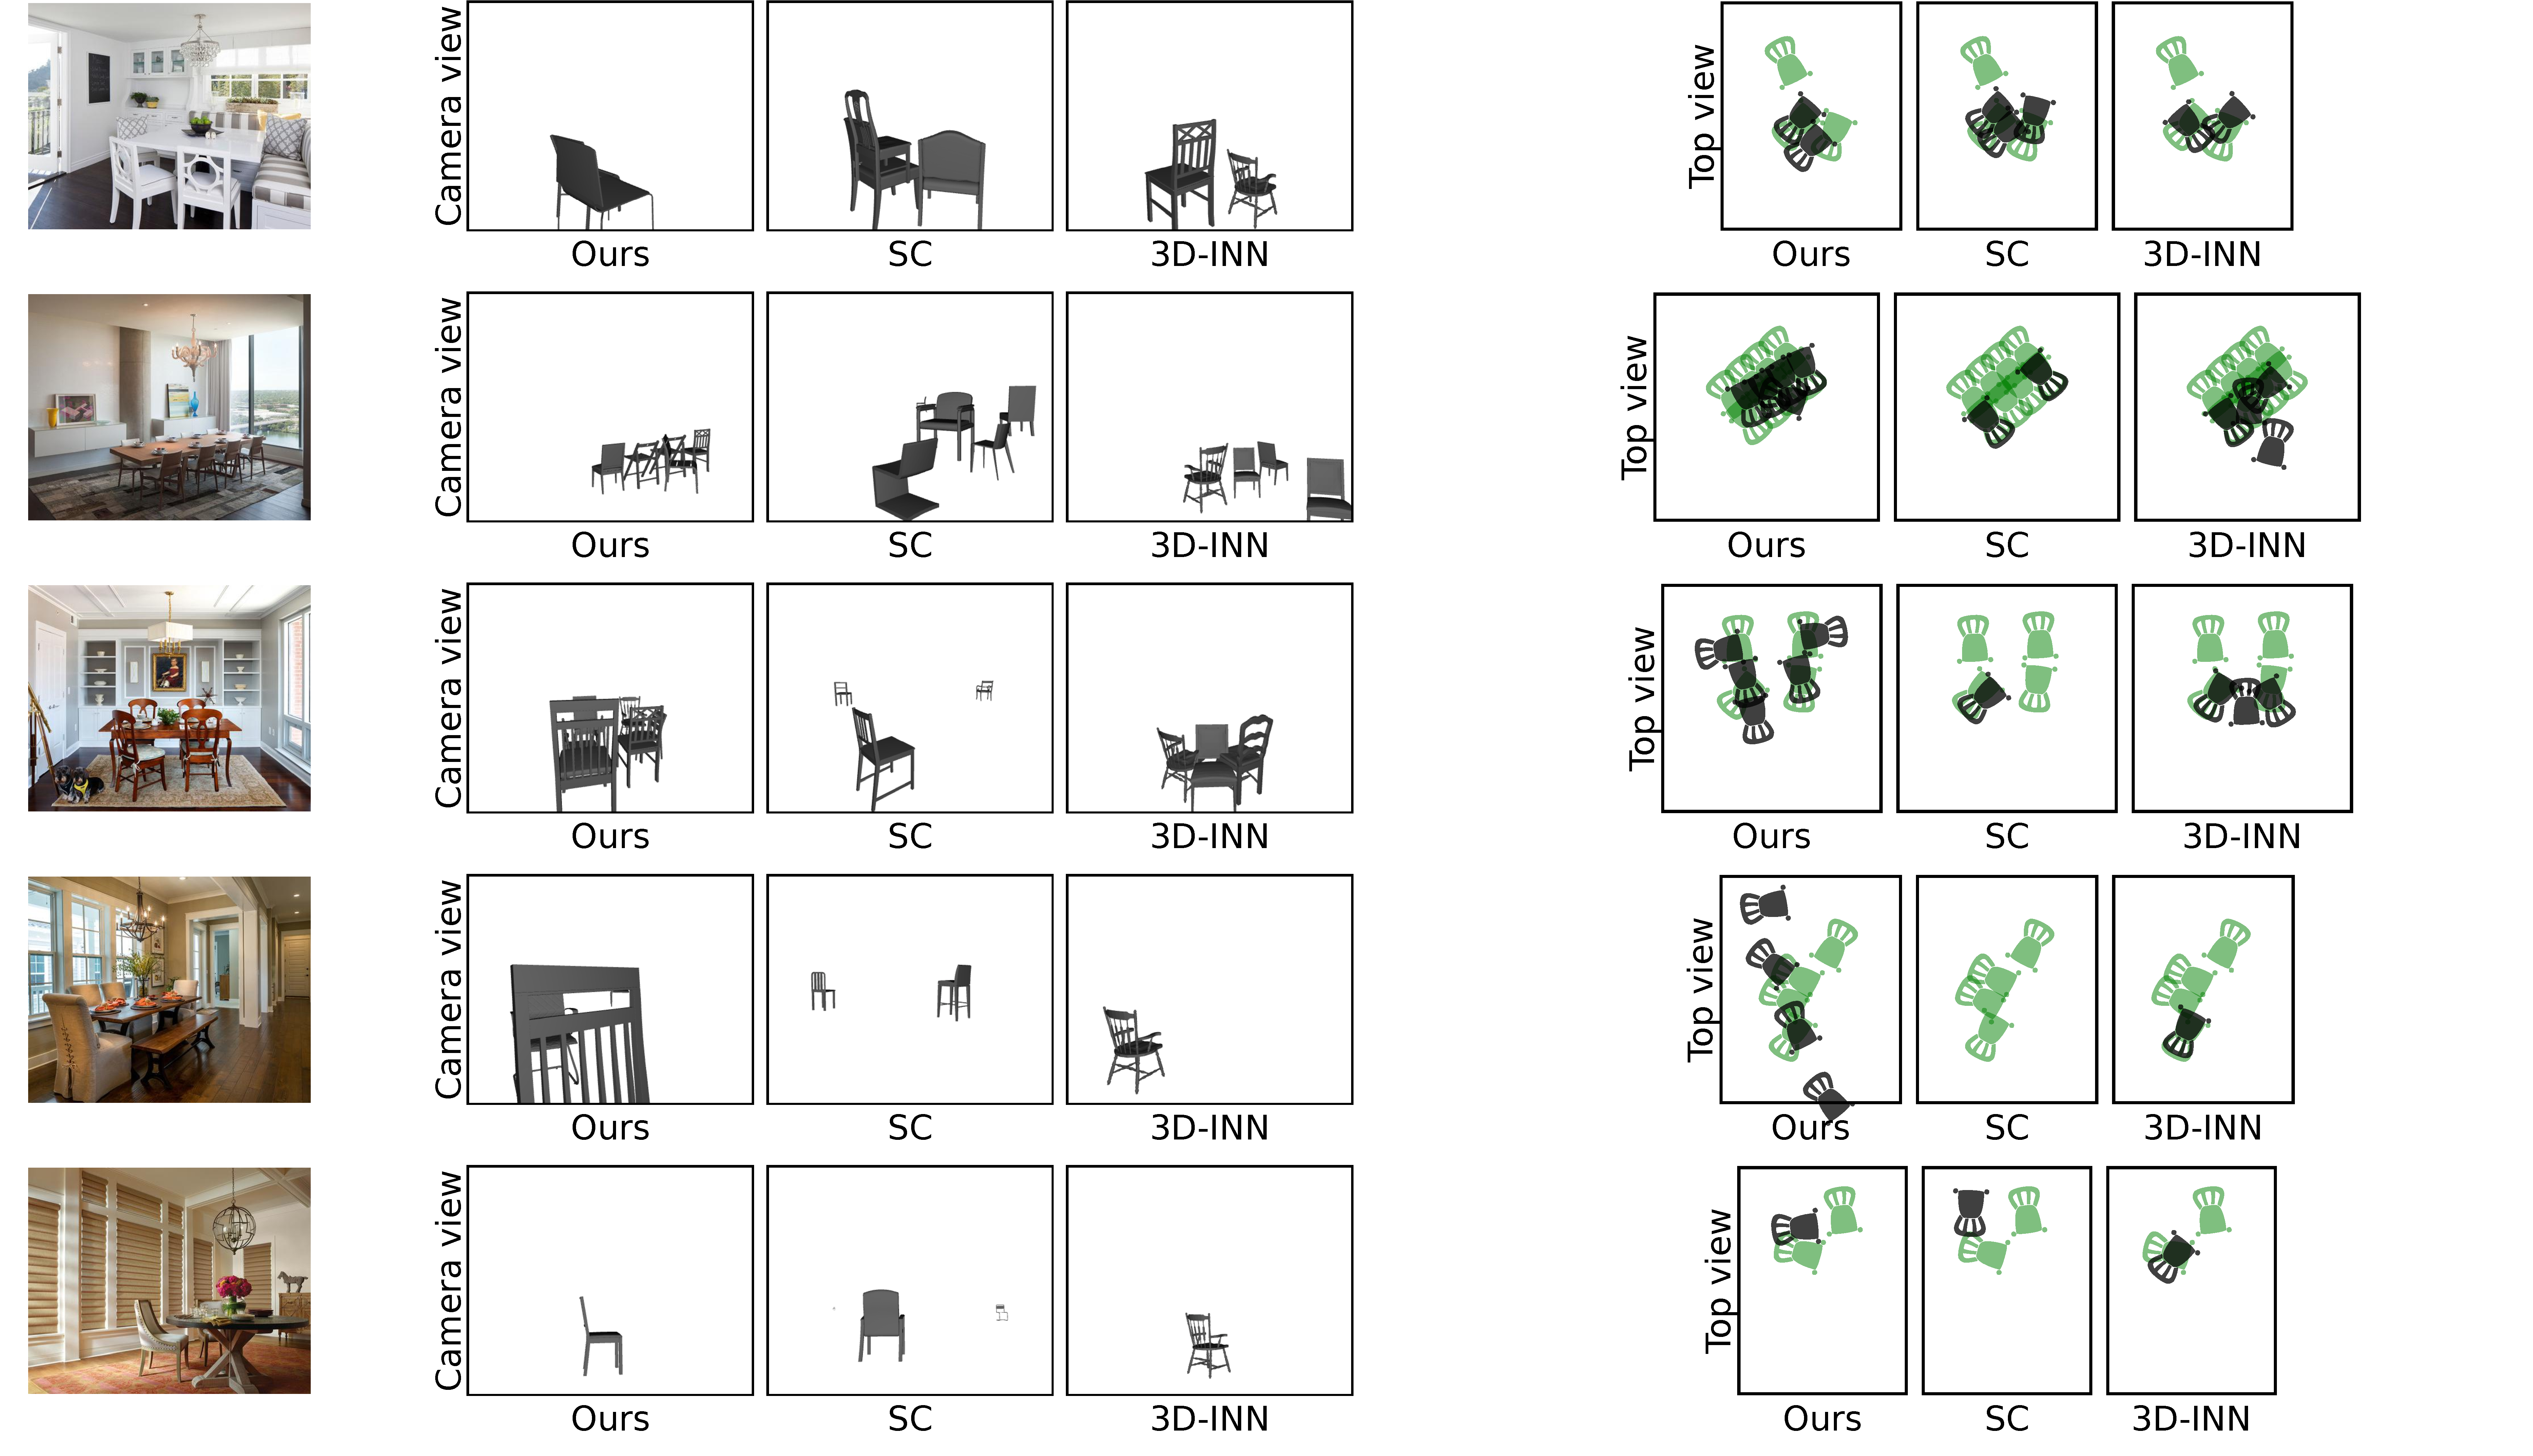
\includegraphics[width=\textwidth]{figures/qualitative_results/full/qual_results_8.pdf}
\end{sidewaysfigure}
\begin{sidewaysfigure}
    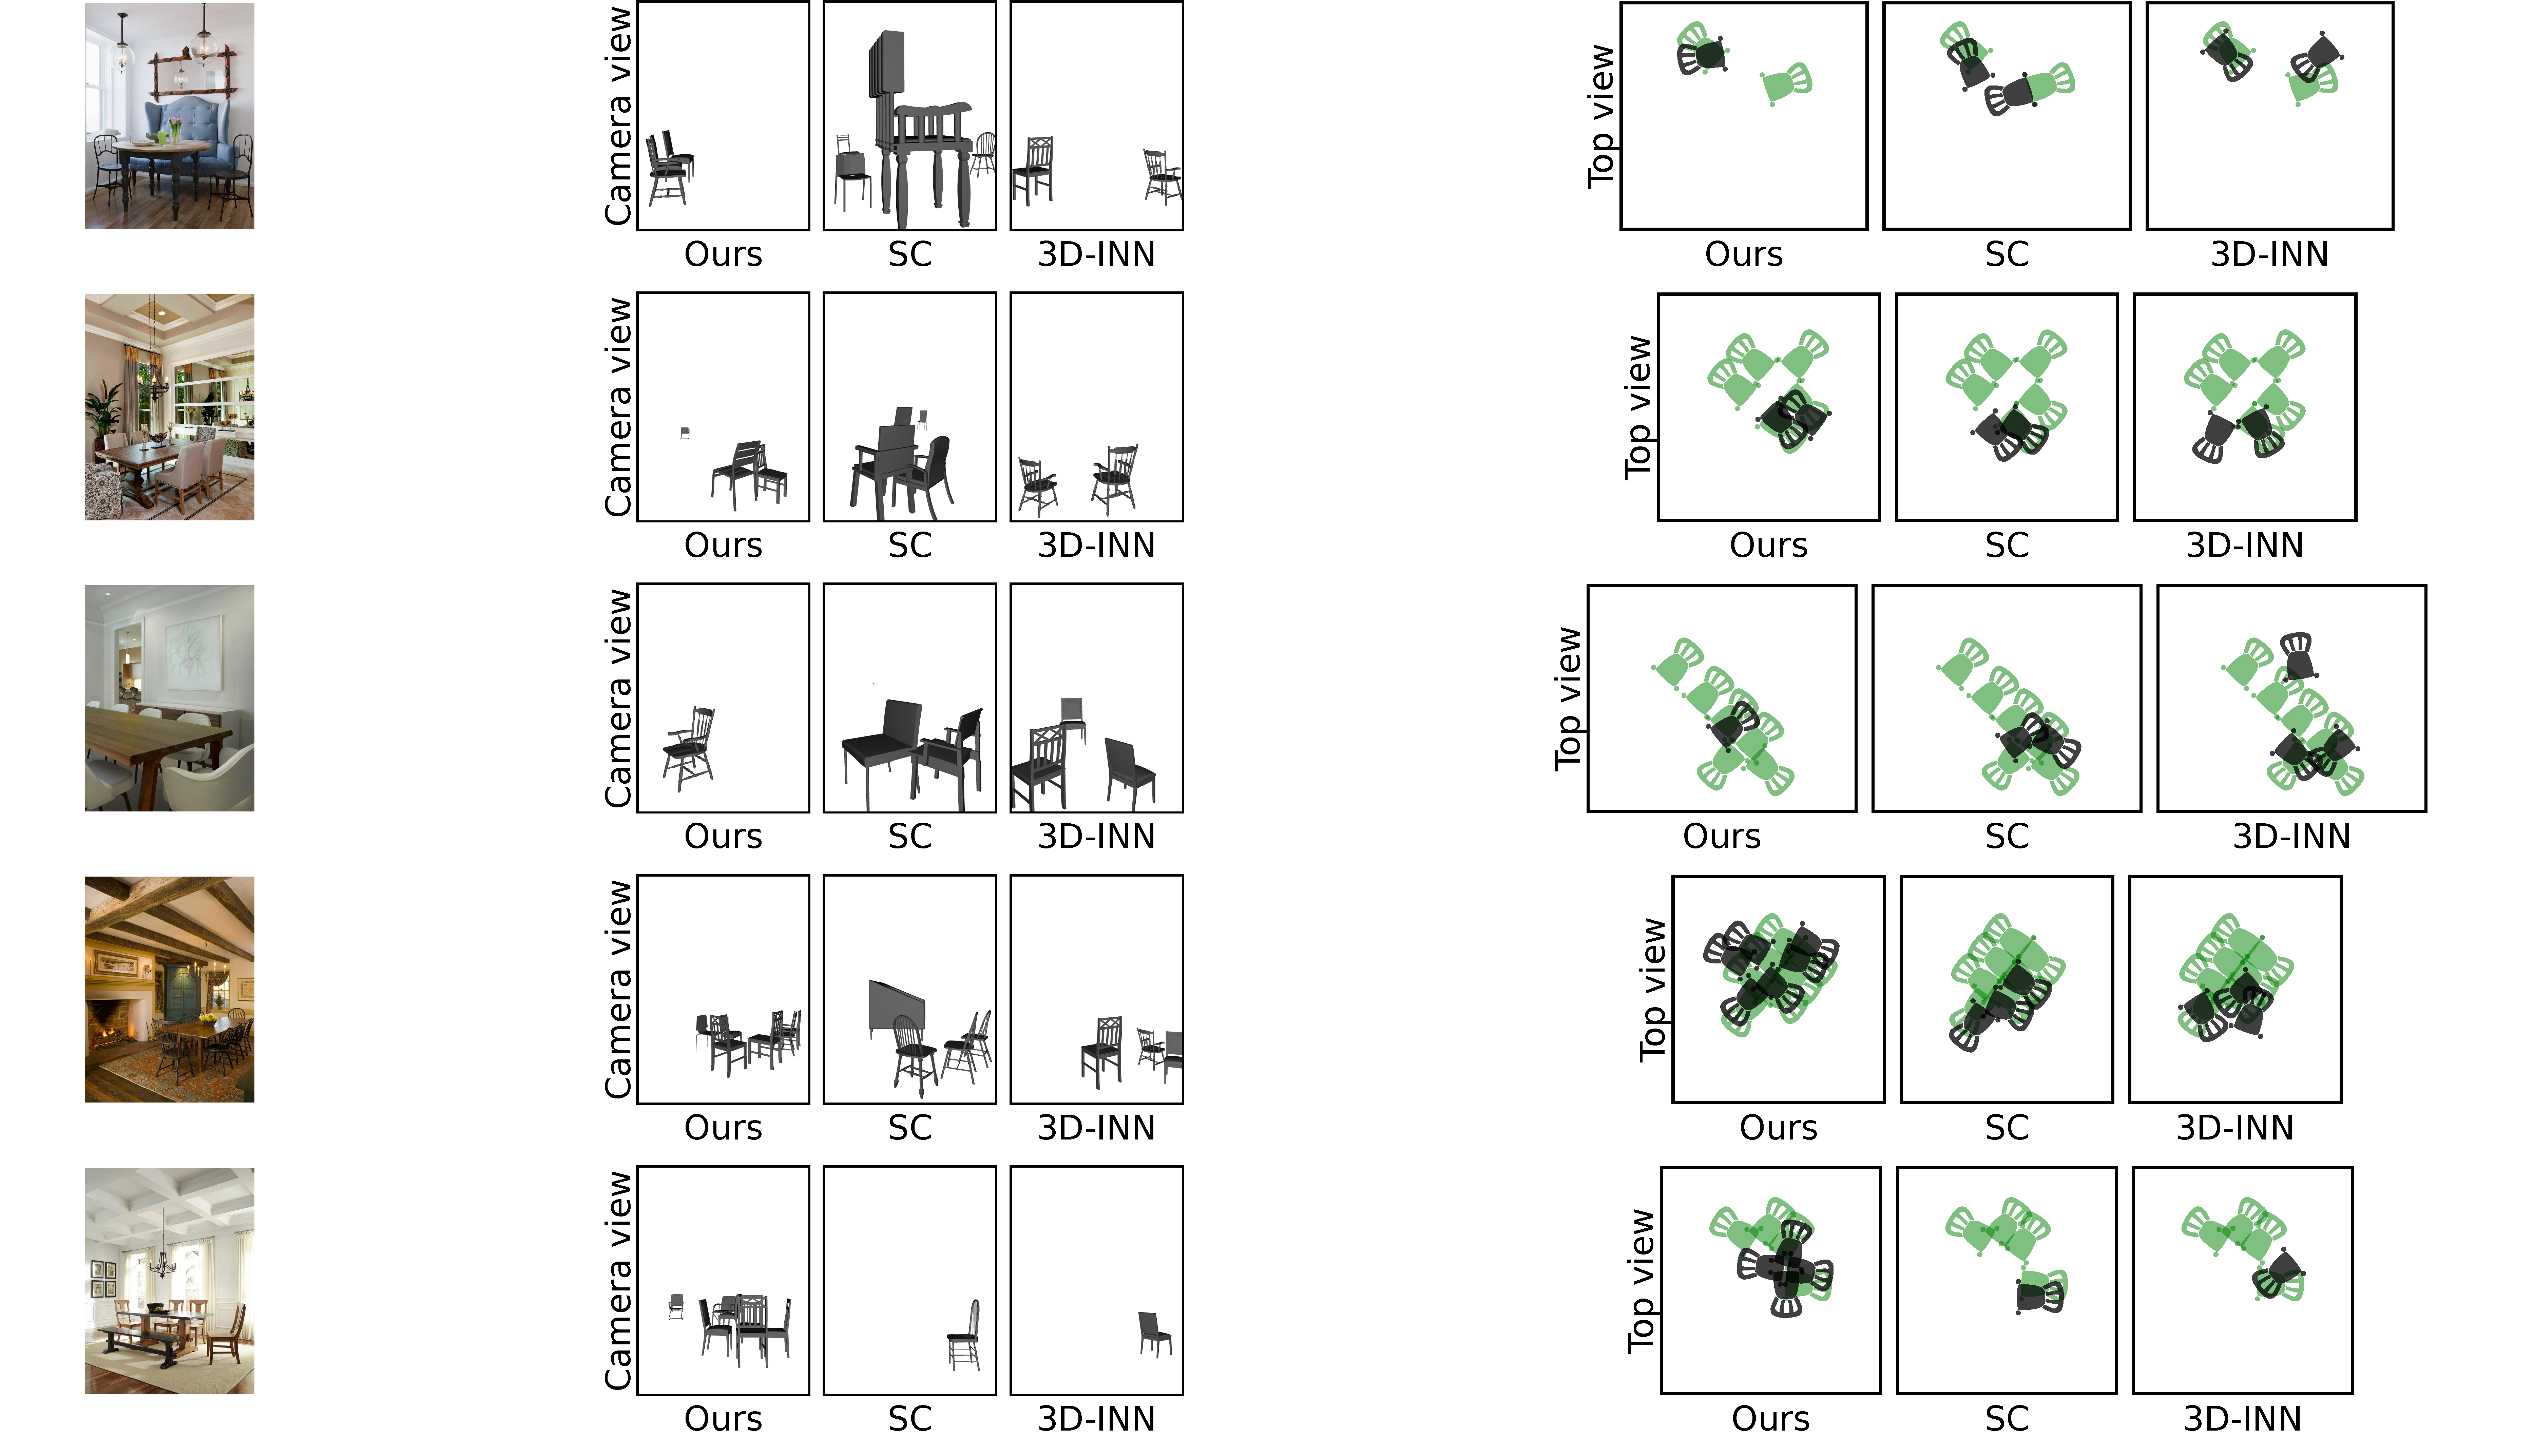
\includegraphics[width=\textwidth]{figures/qualitative_results/full/qual_results_9.pdf}
\end{sidewaysfigure}
\begin{sidewaysfigure}
    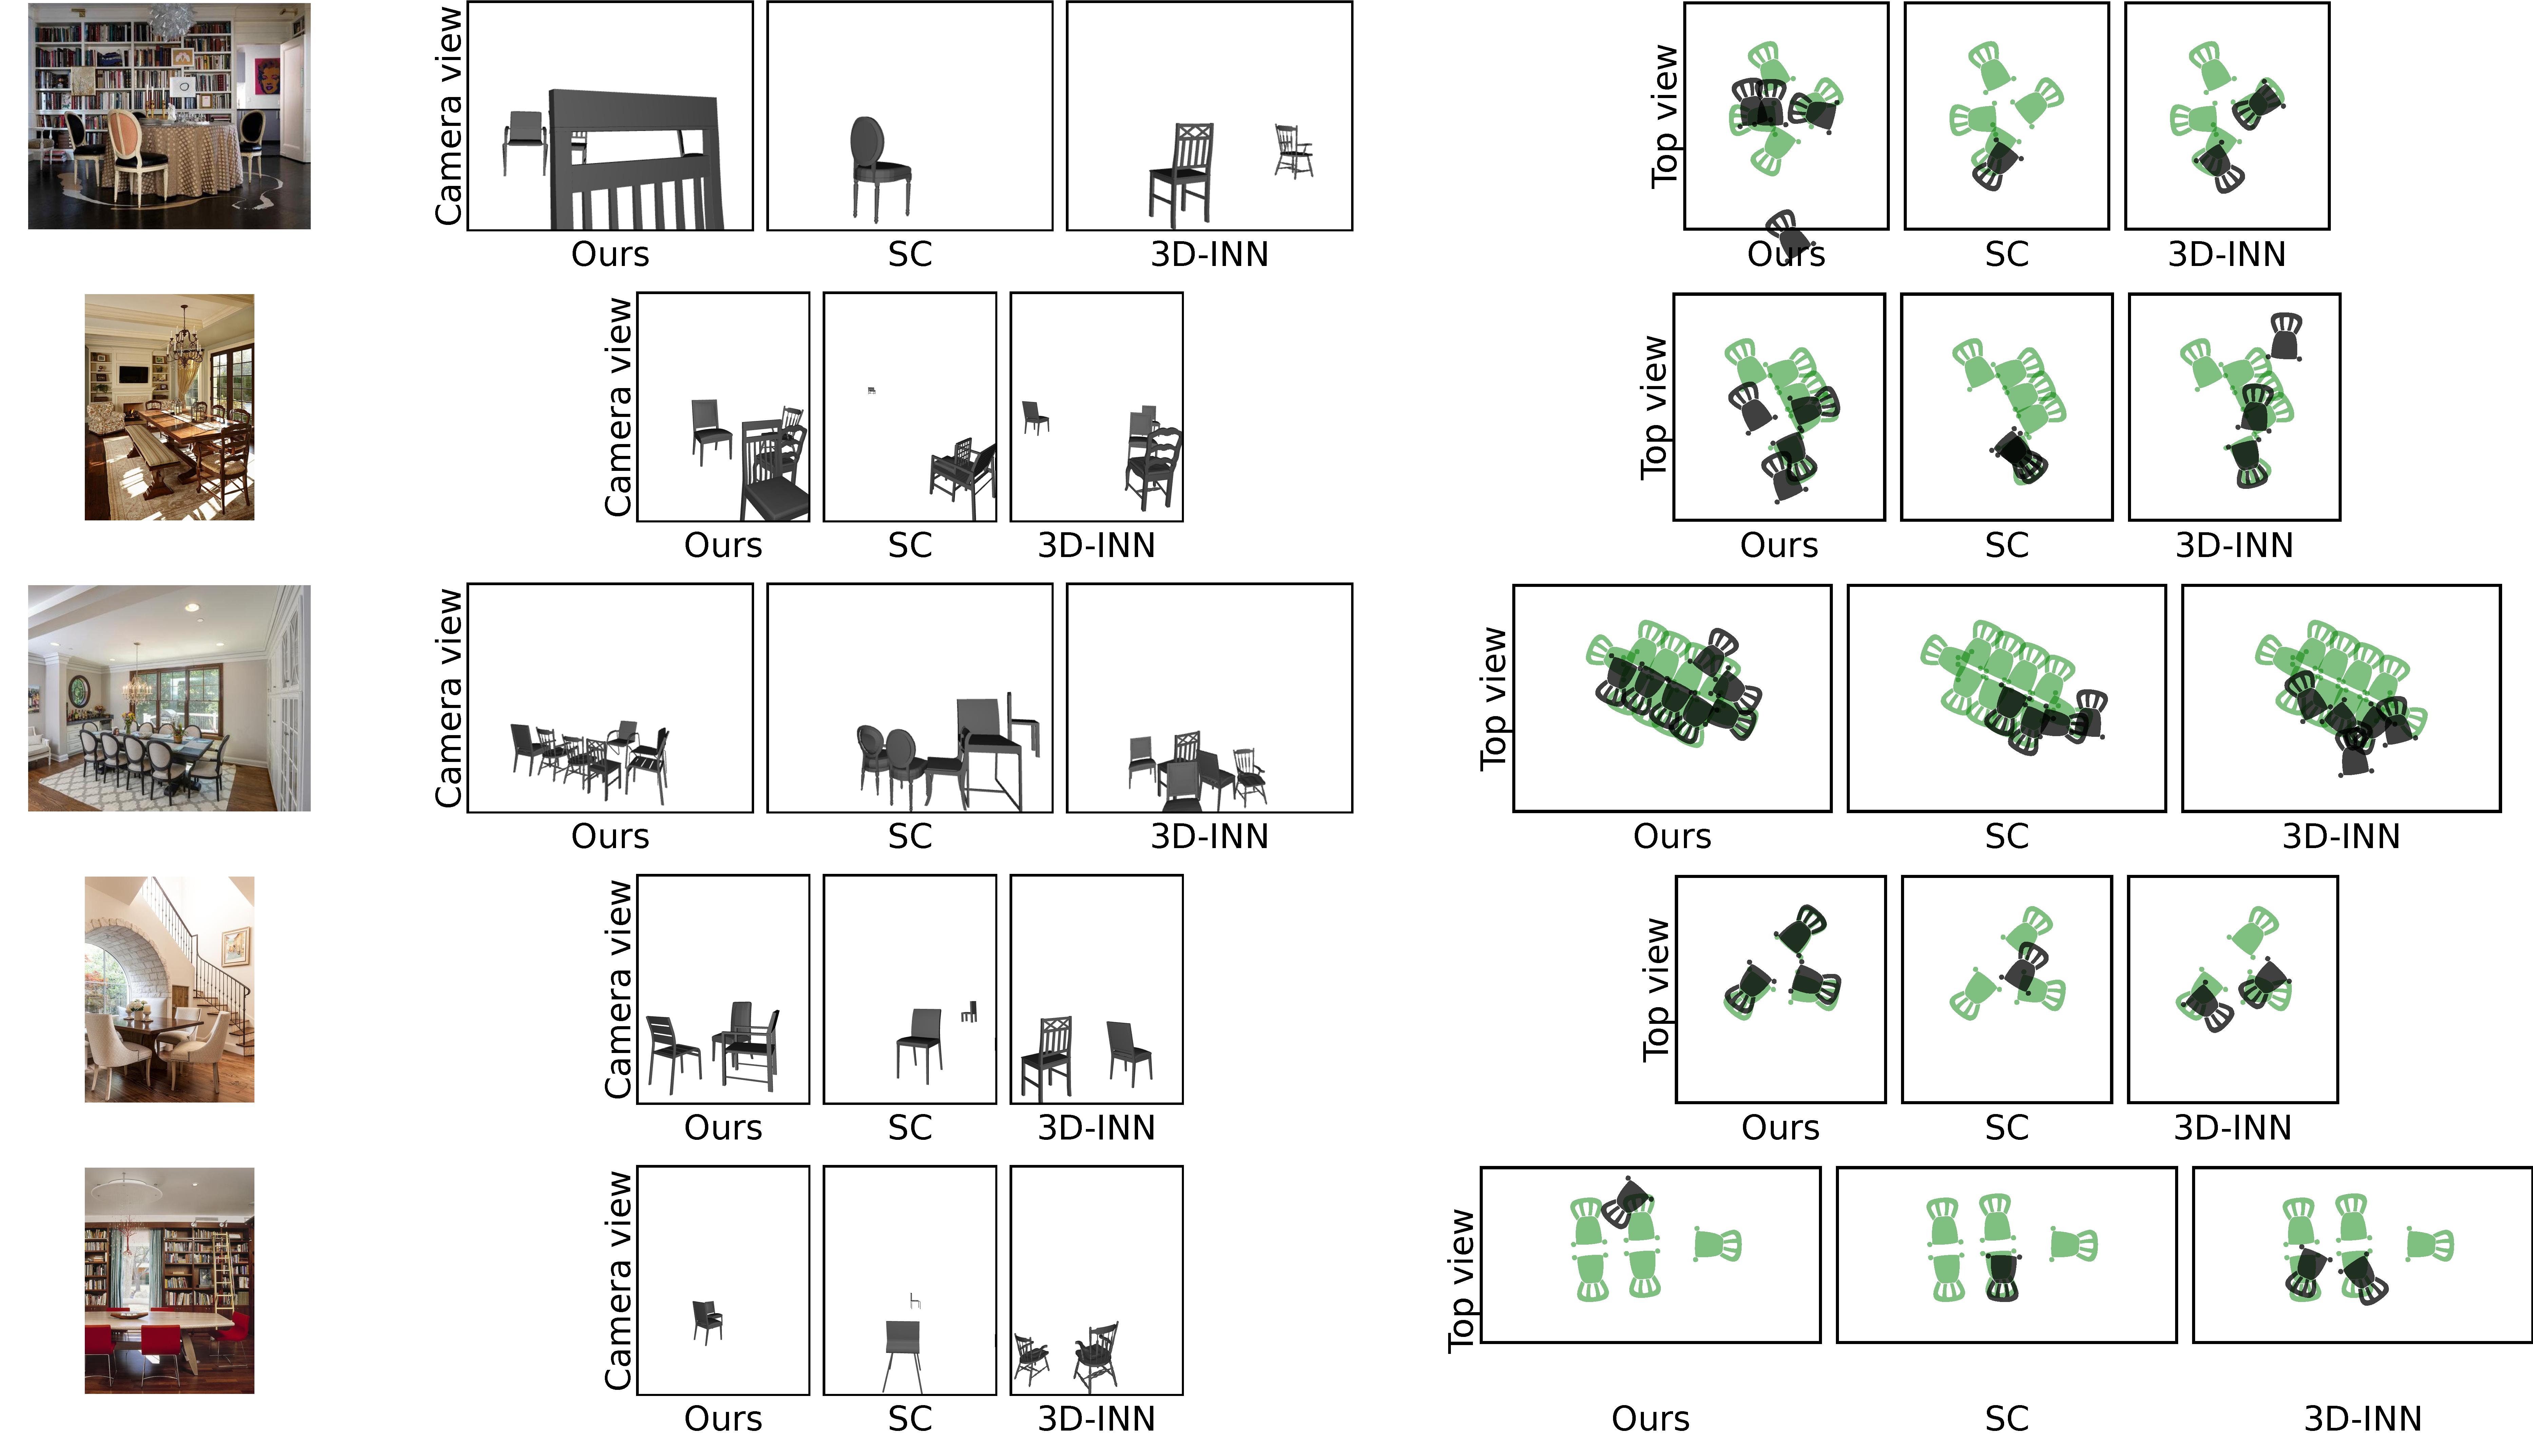
\includegraphics[width=\textwidth]{figures/qualitative_results/full/qual_results_10.pdf}
\end{sidewaysfigure}
\begin{sidewaysfigure}
    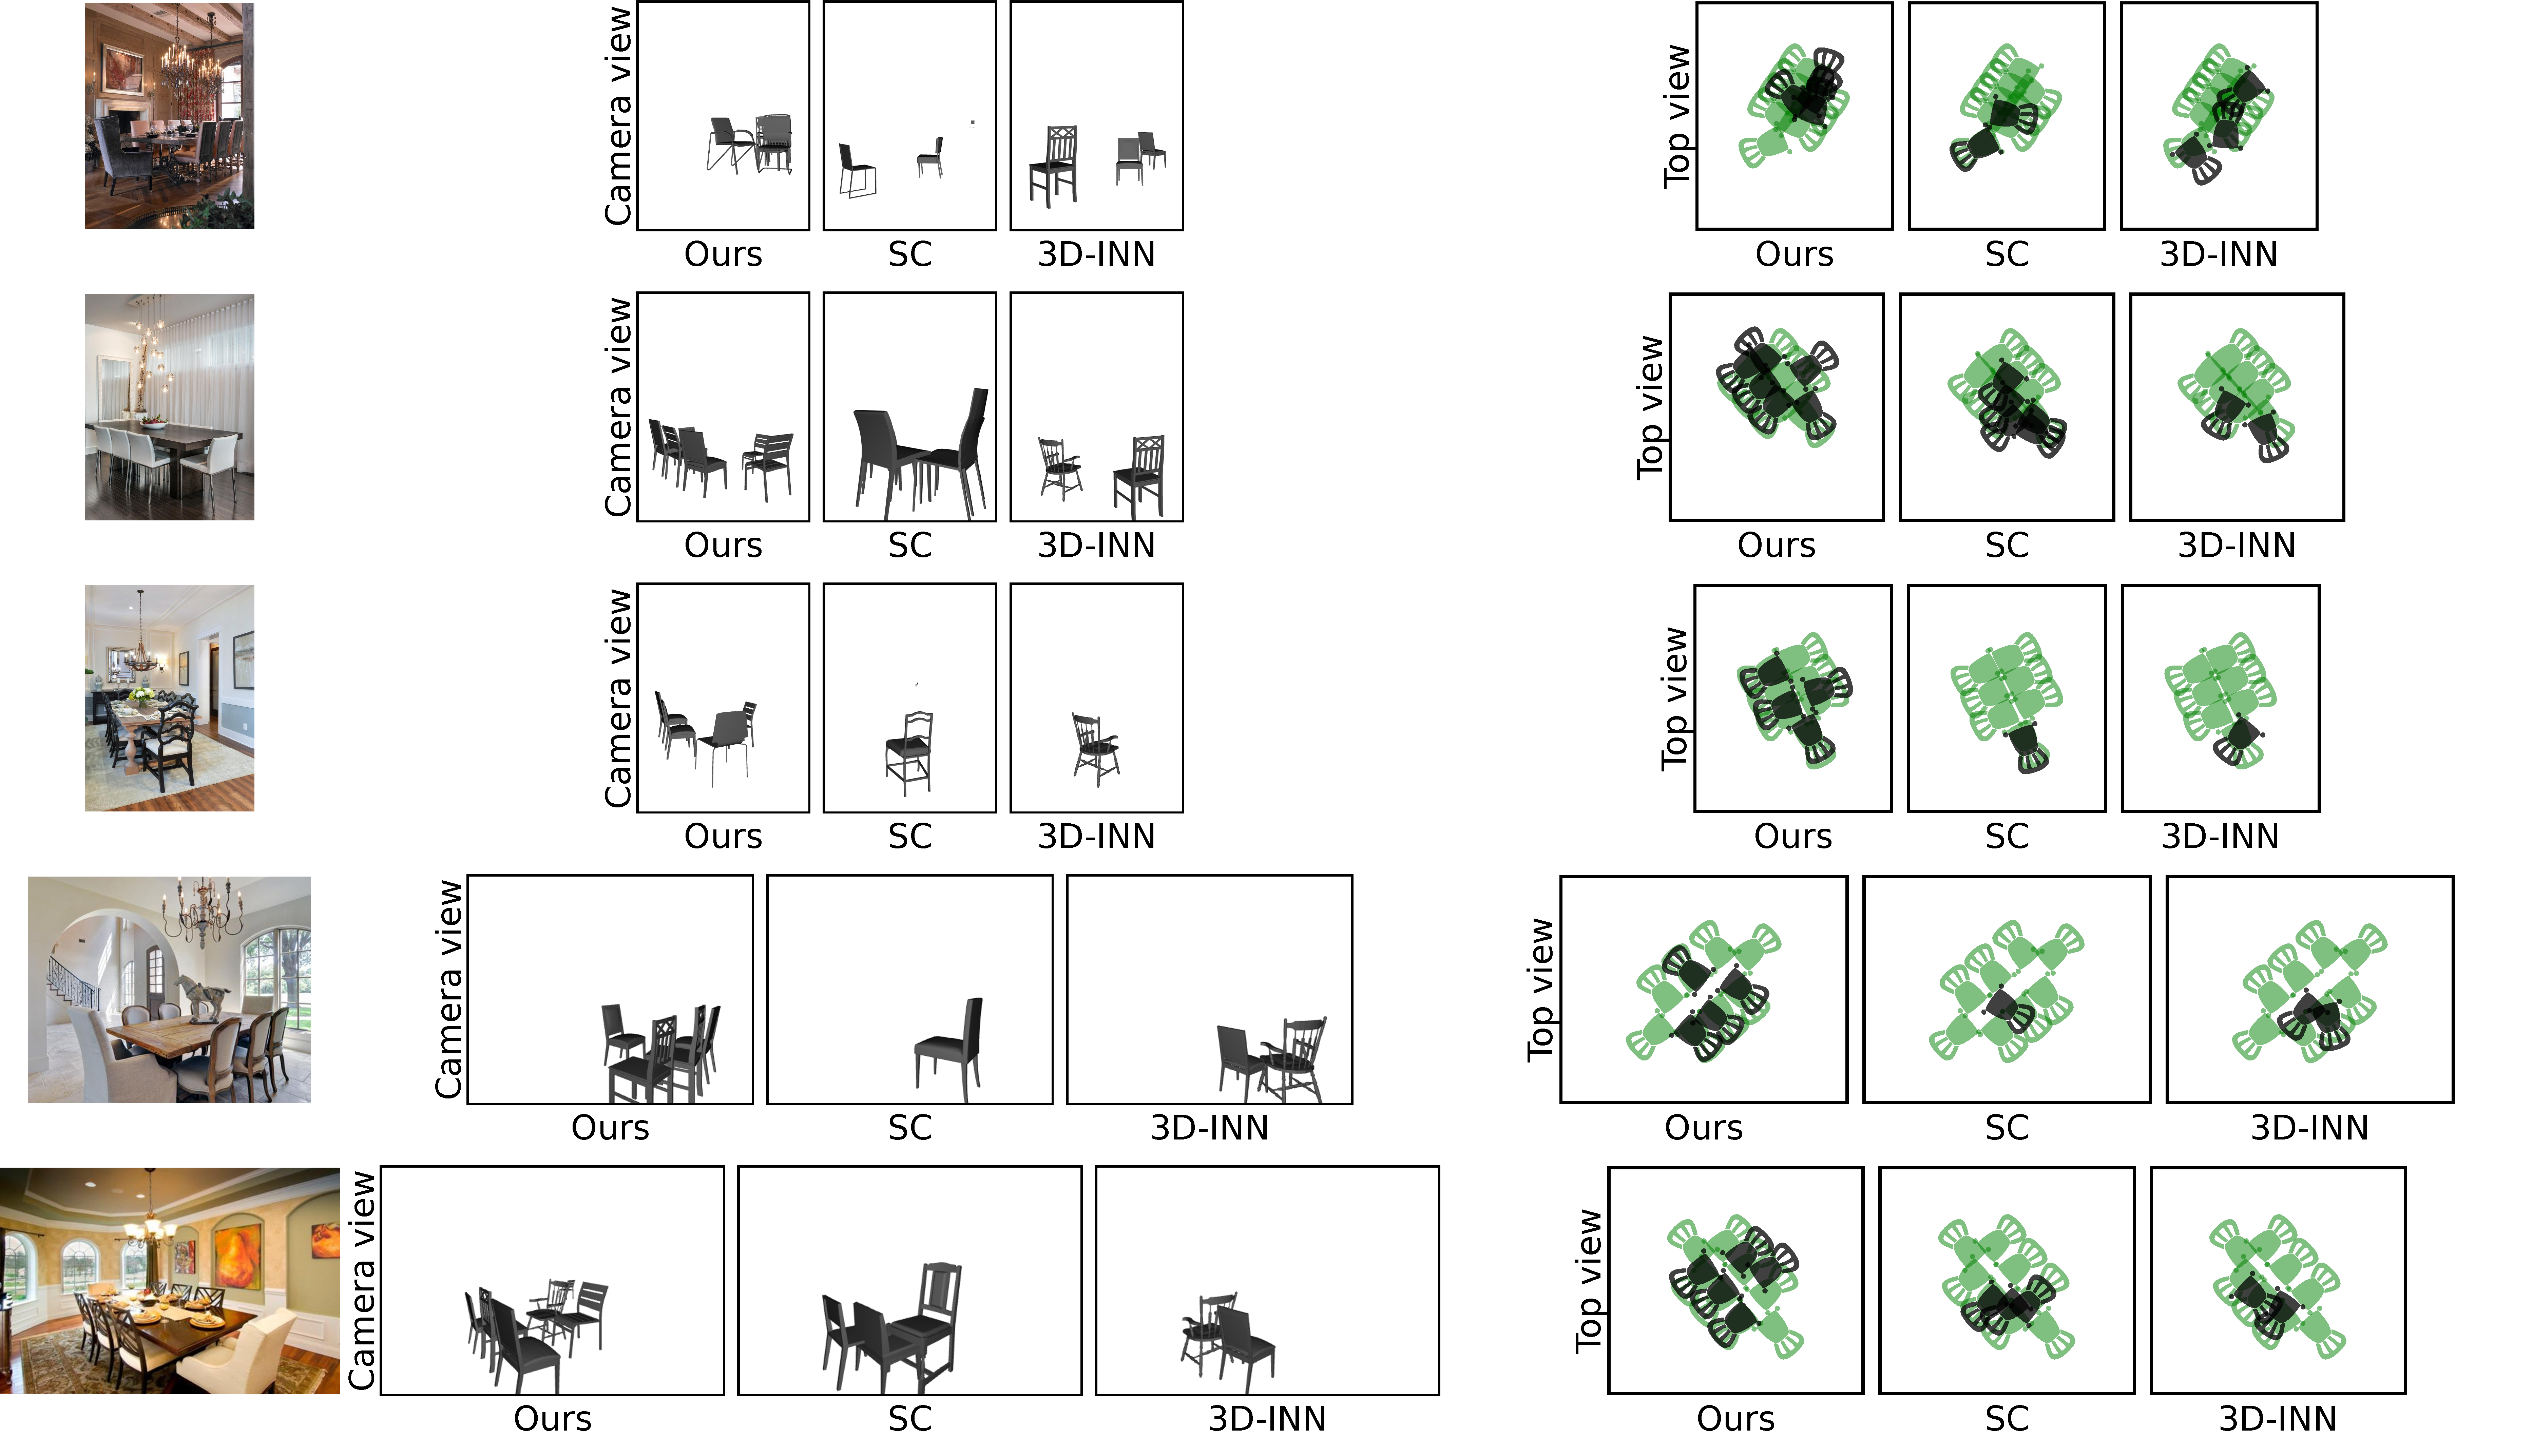
\includegraphics[width=\textwidth]{figures/qualitative_results/full/qual_results_11.pdf}
\end{sidewaysfigure}
\begin{sidewaysfigure}
    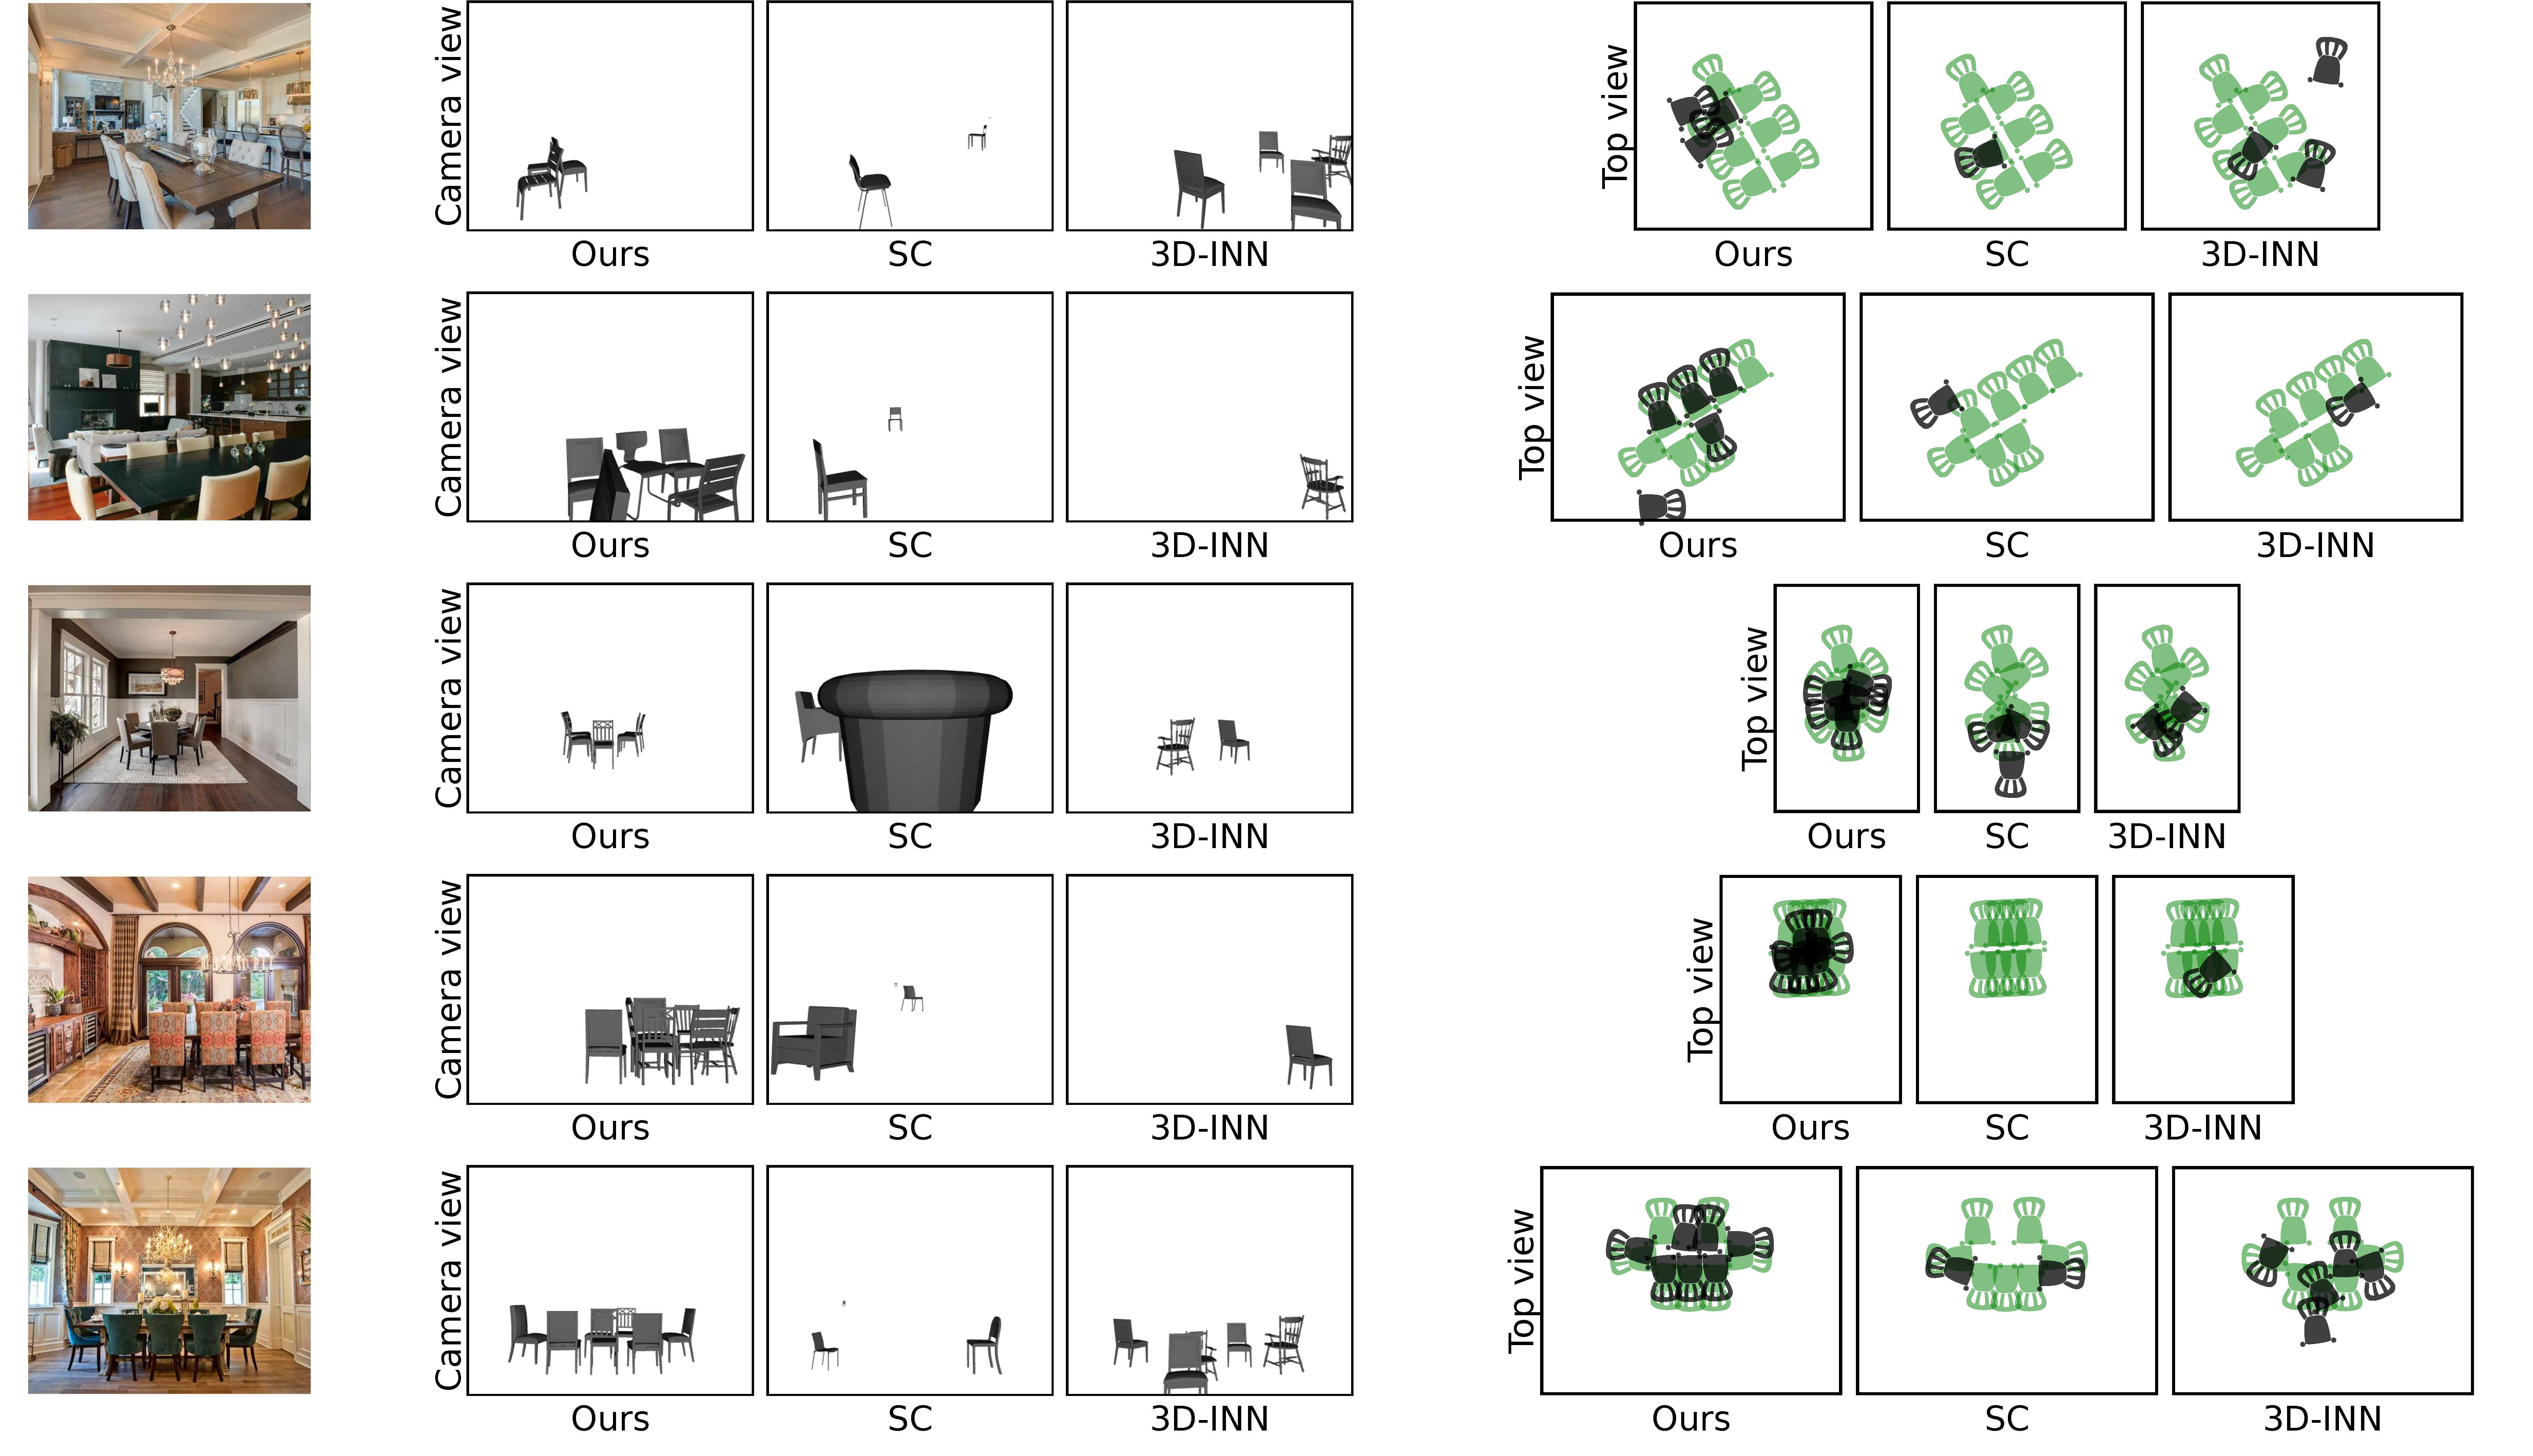
\includegraphics[width=\textwidth]{figures/qualitative_results/full/qual_results_12.pdf}
\end{sidewaysfigure}
\begin{sidewaysfigure}
    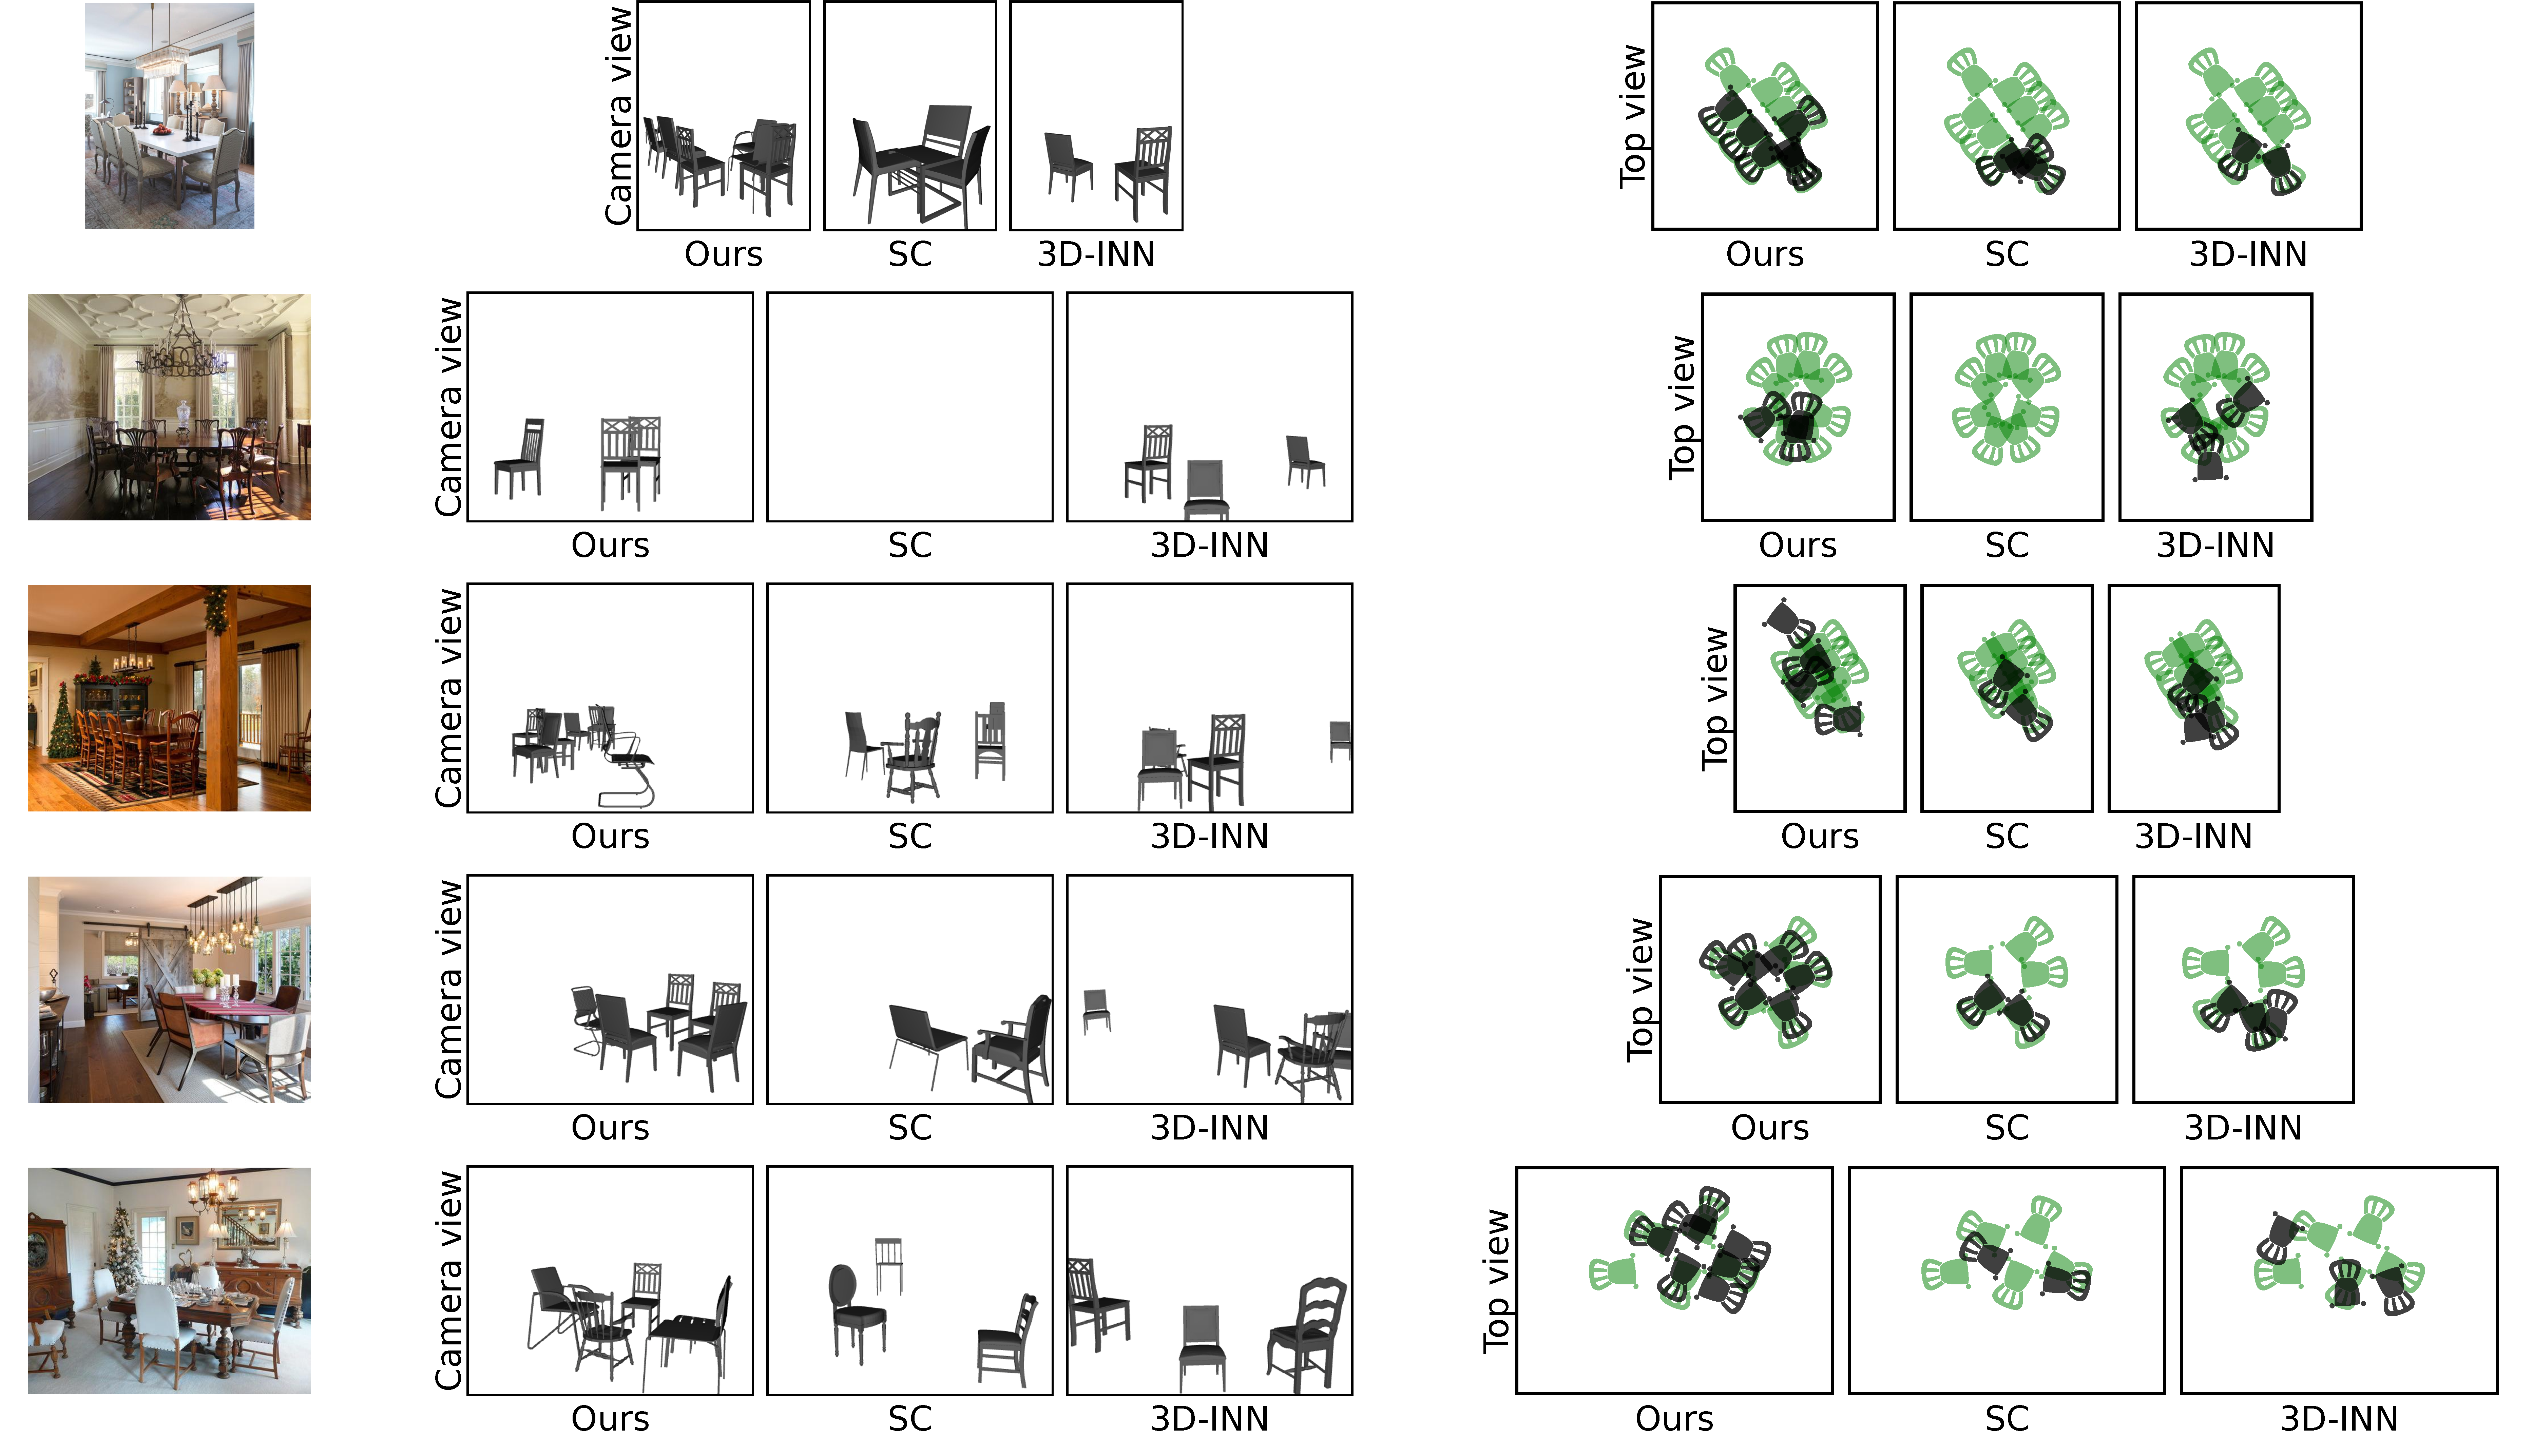
\includegraphics[width=\textwidth]{figures/qualitative_results/full/qual_results_13.pdf}
\end{sidewaysfigure}
\begin{sidewaysfigure}
    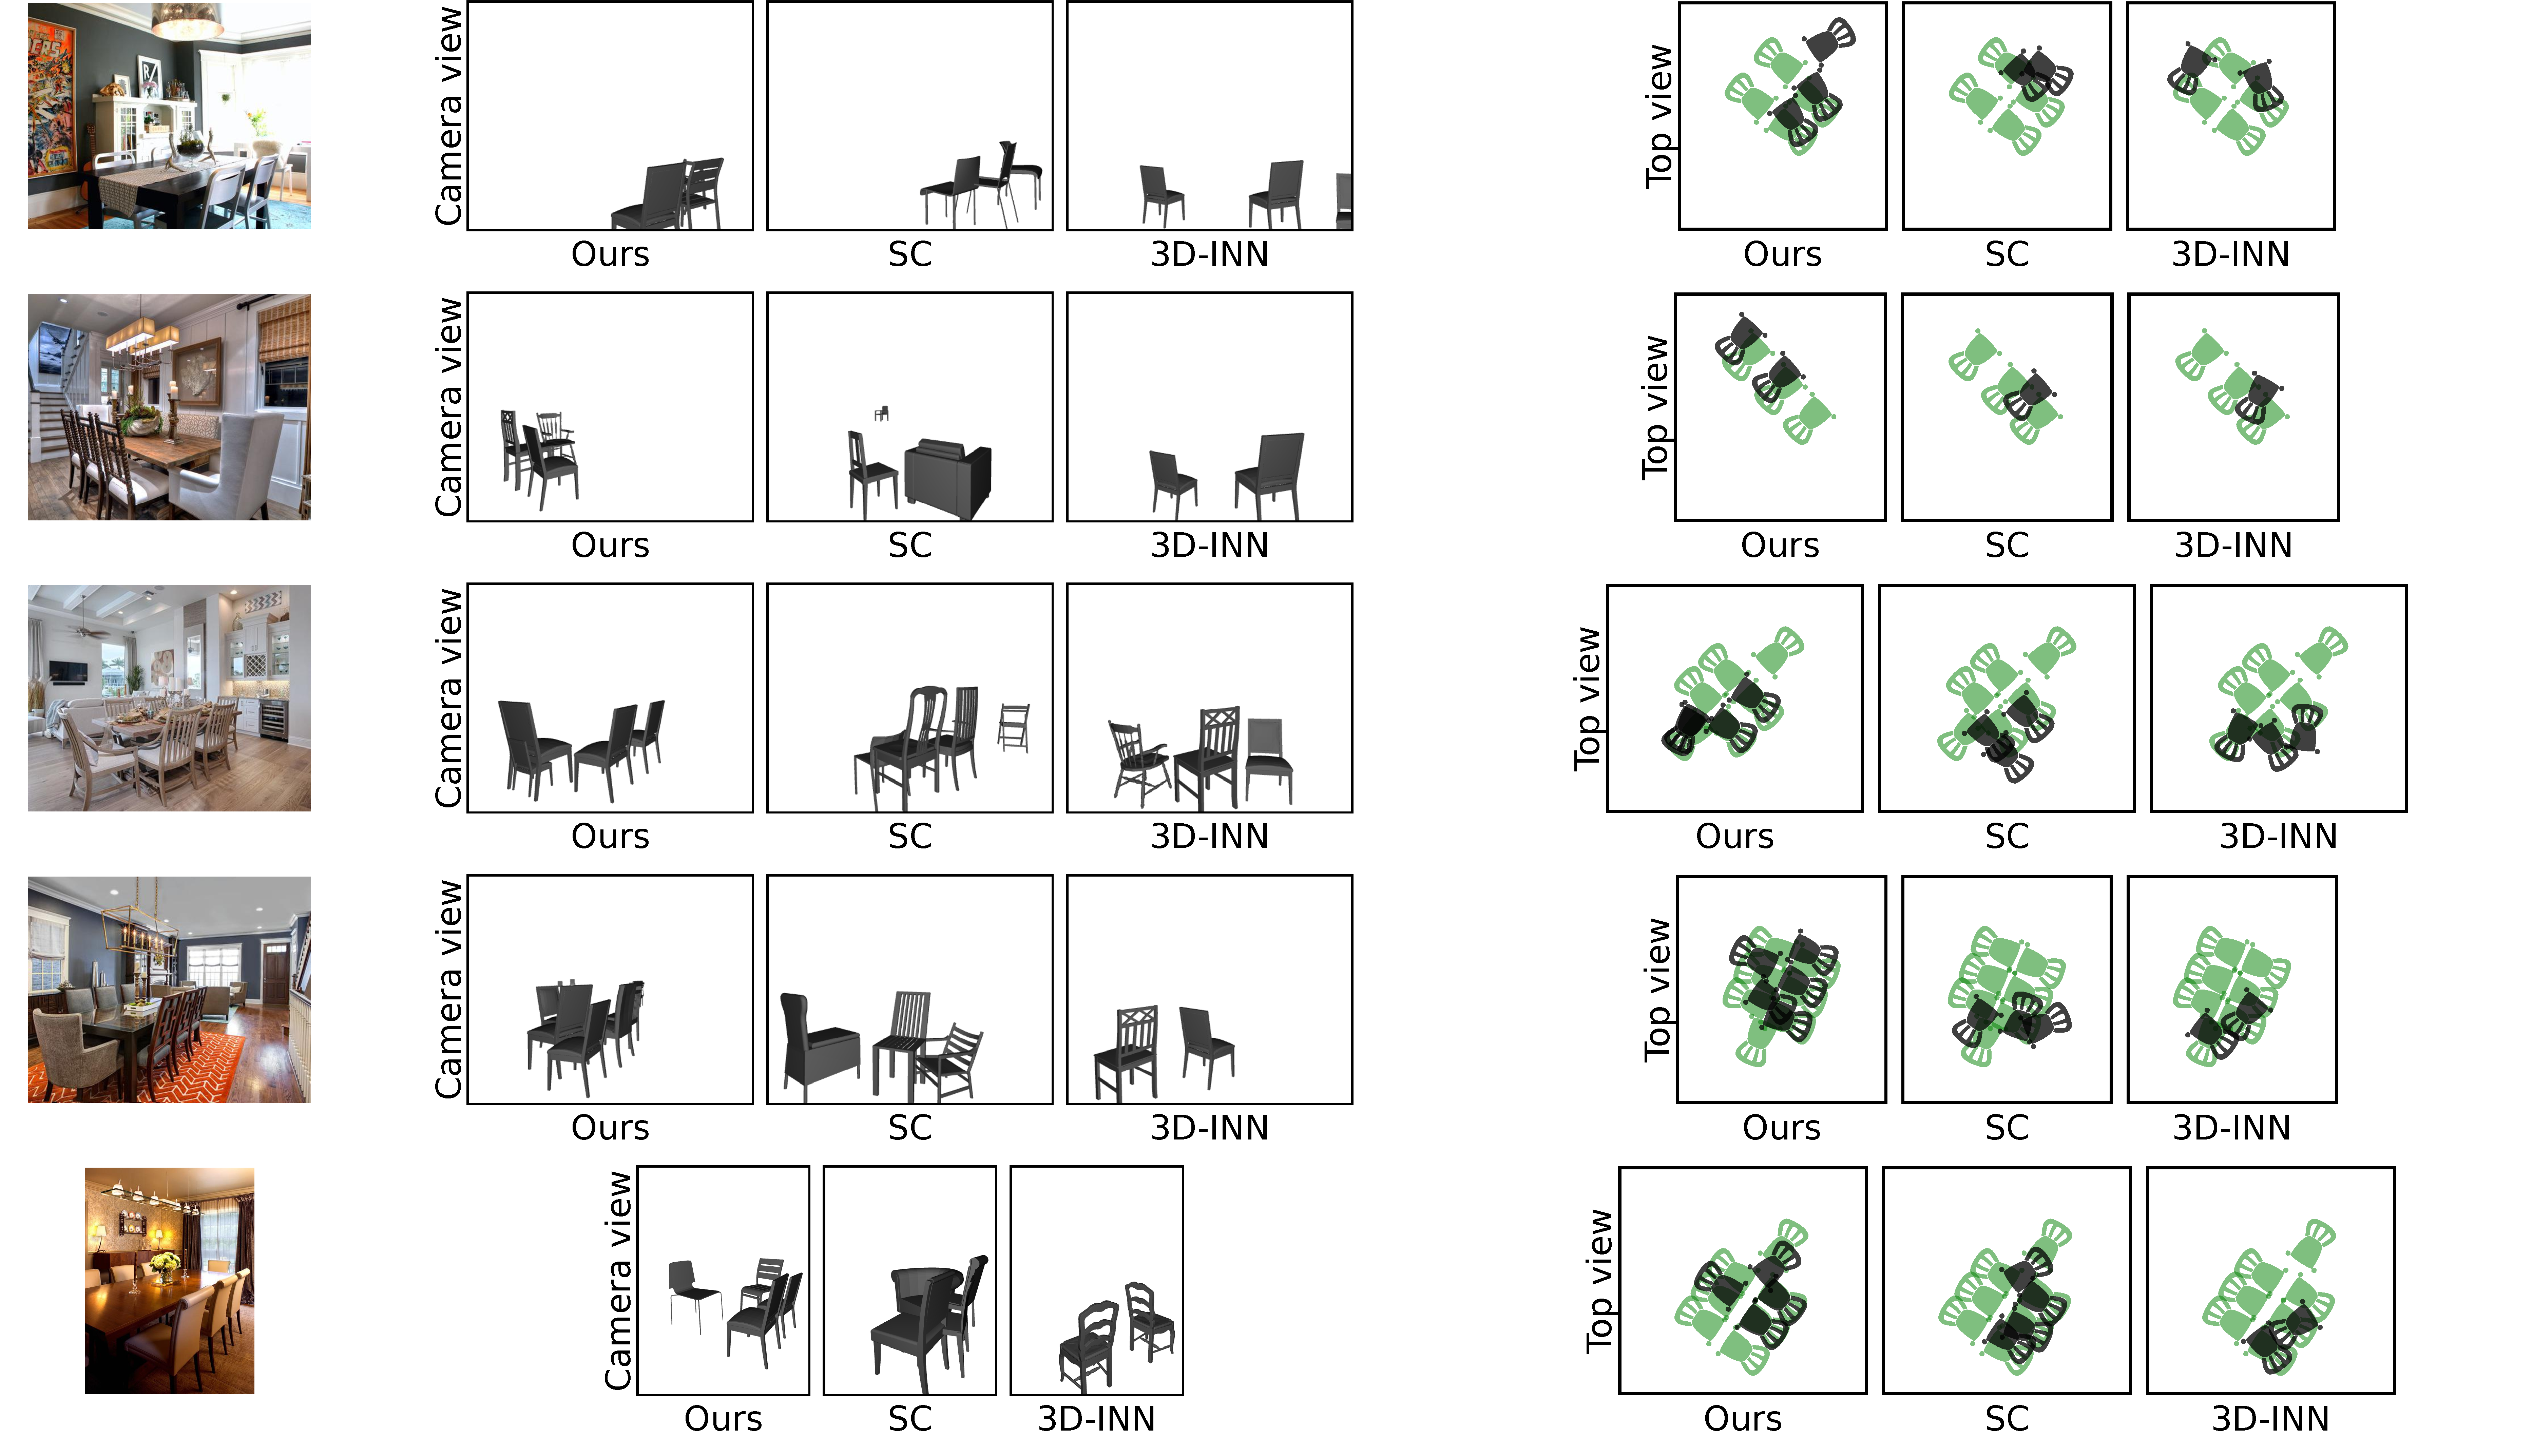
\includegraphics[width=\textwidth]{figures/qualitative_results/full/qual_results_14.pdf}
\end{sidewaysfigure}
\begin{sidewaysfigure}
    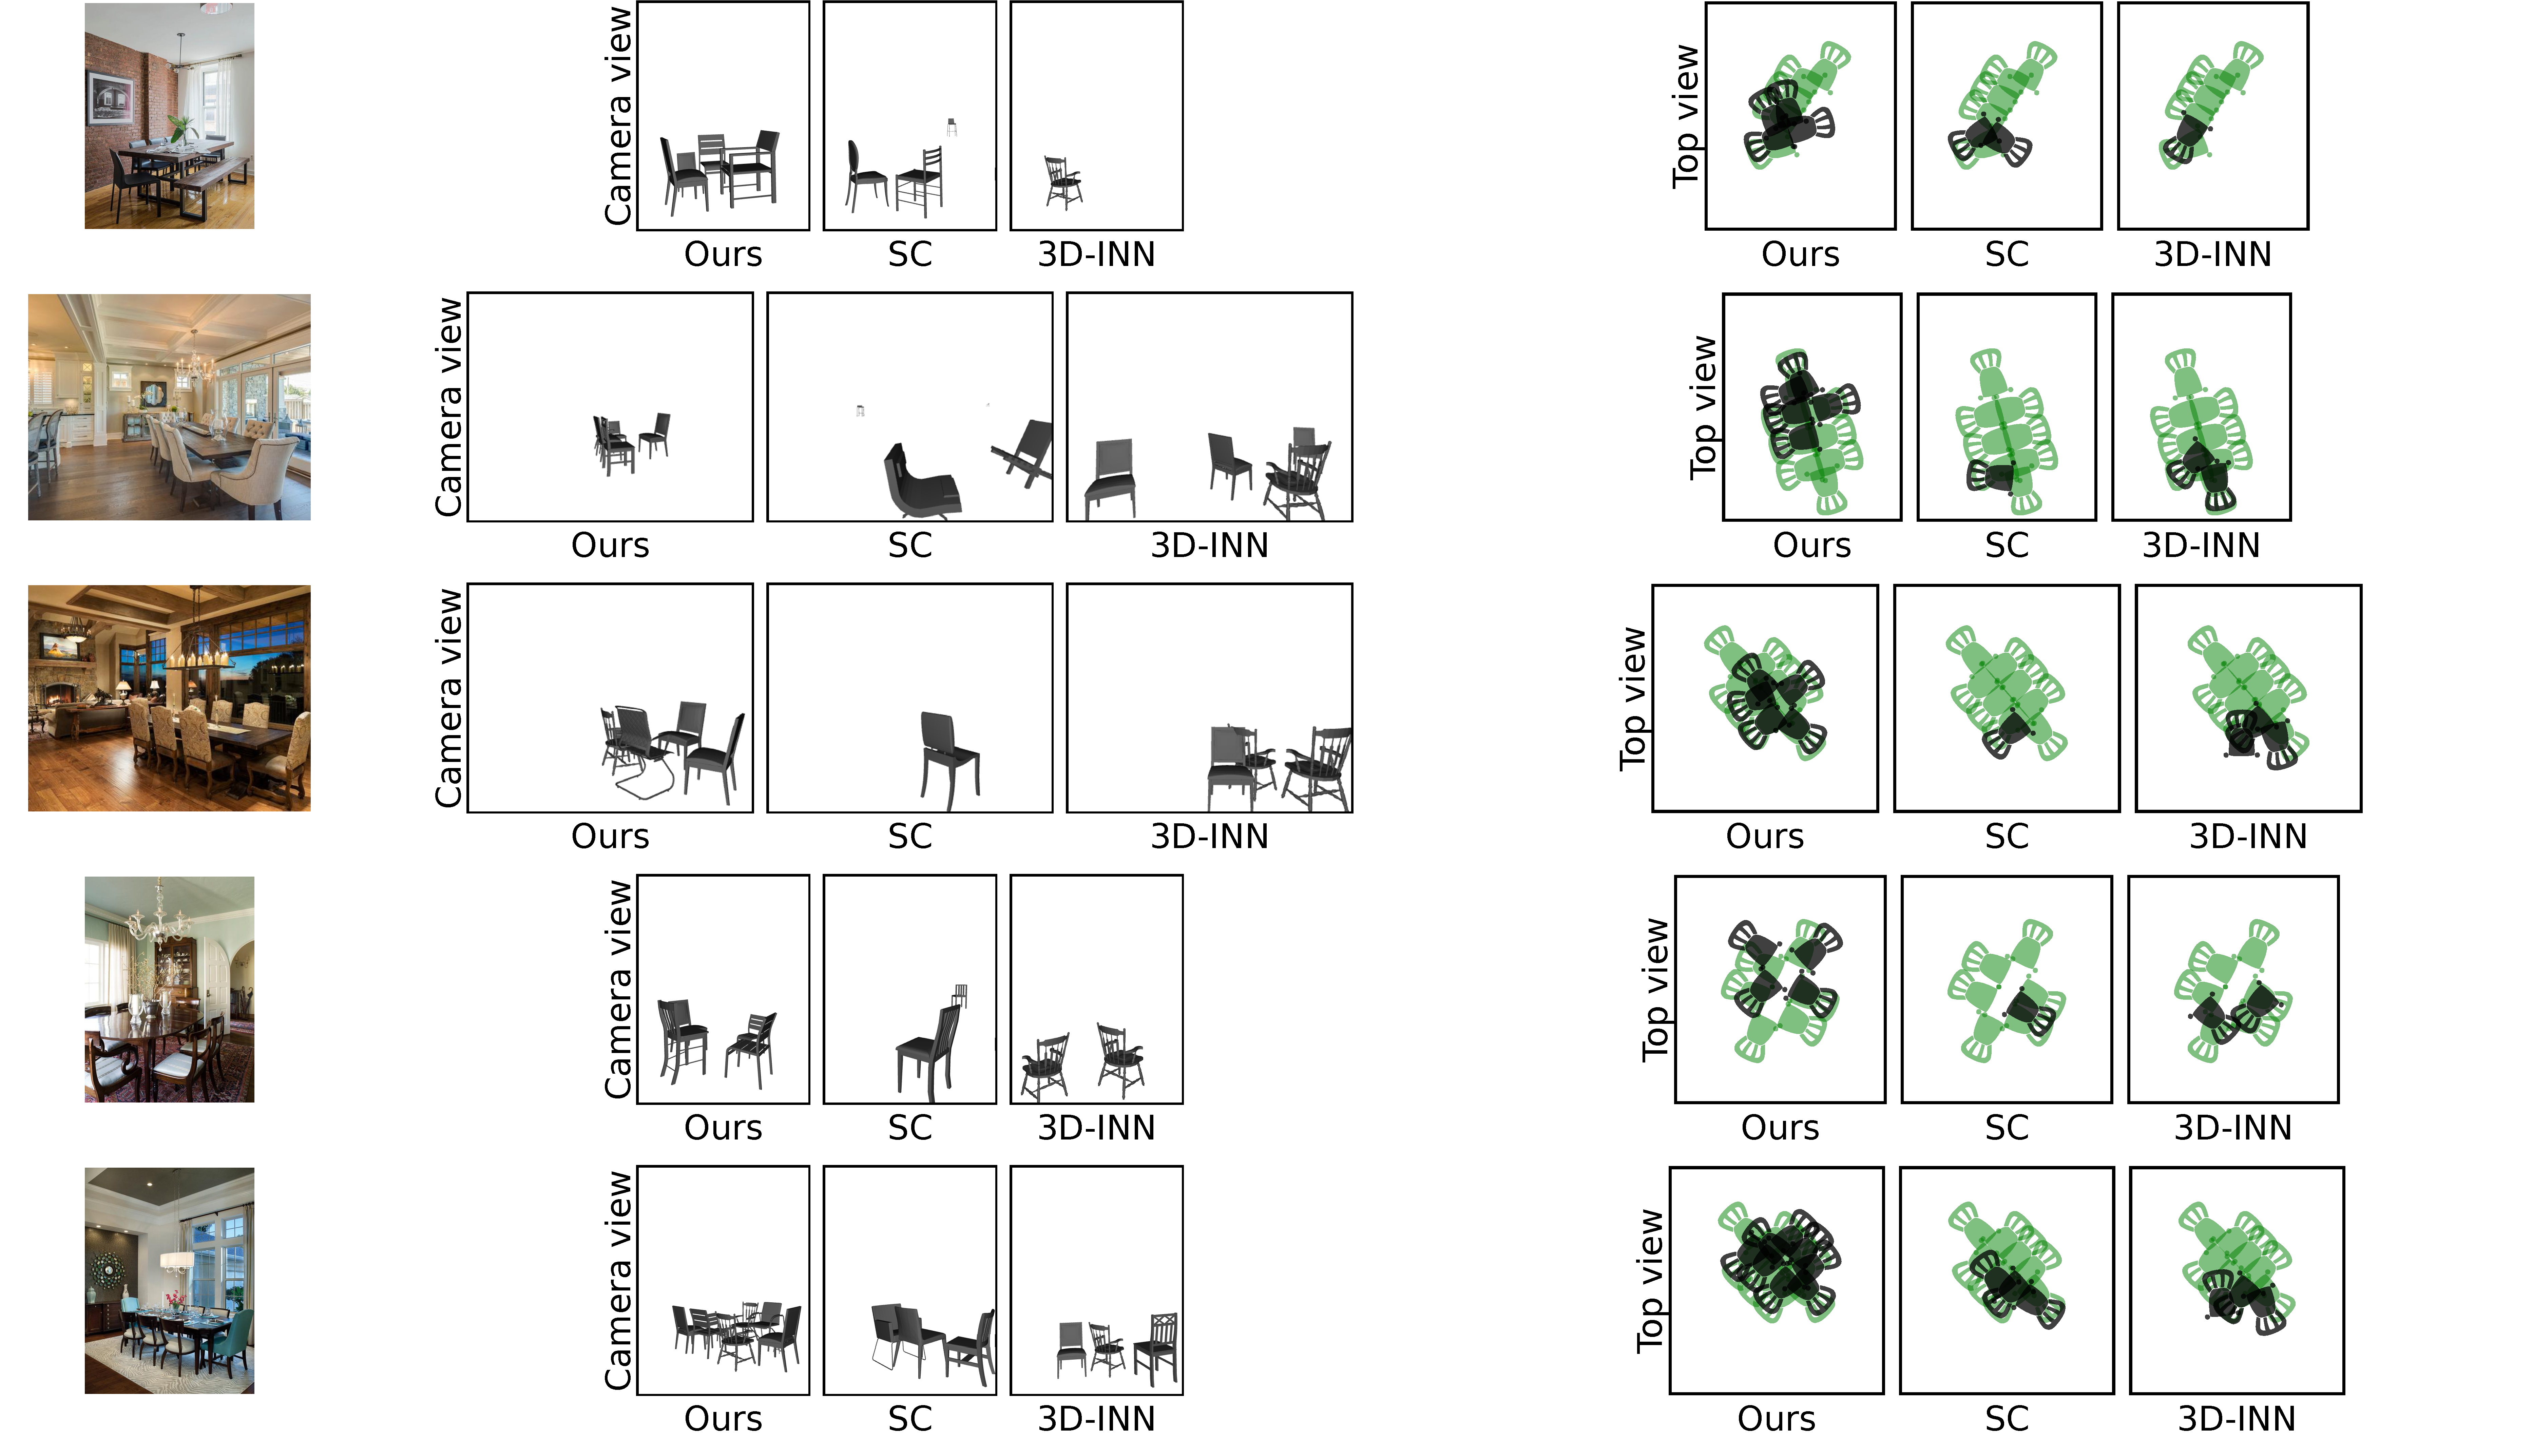
\includegraphics[width=\textwidth]{figures/qualitative_results/full/qual_results_15.pdf}
\end{sidewaysfigure}
\begin{sidewaysfigure}
    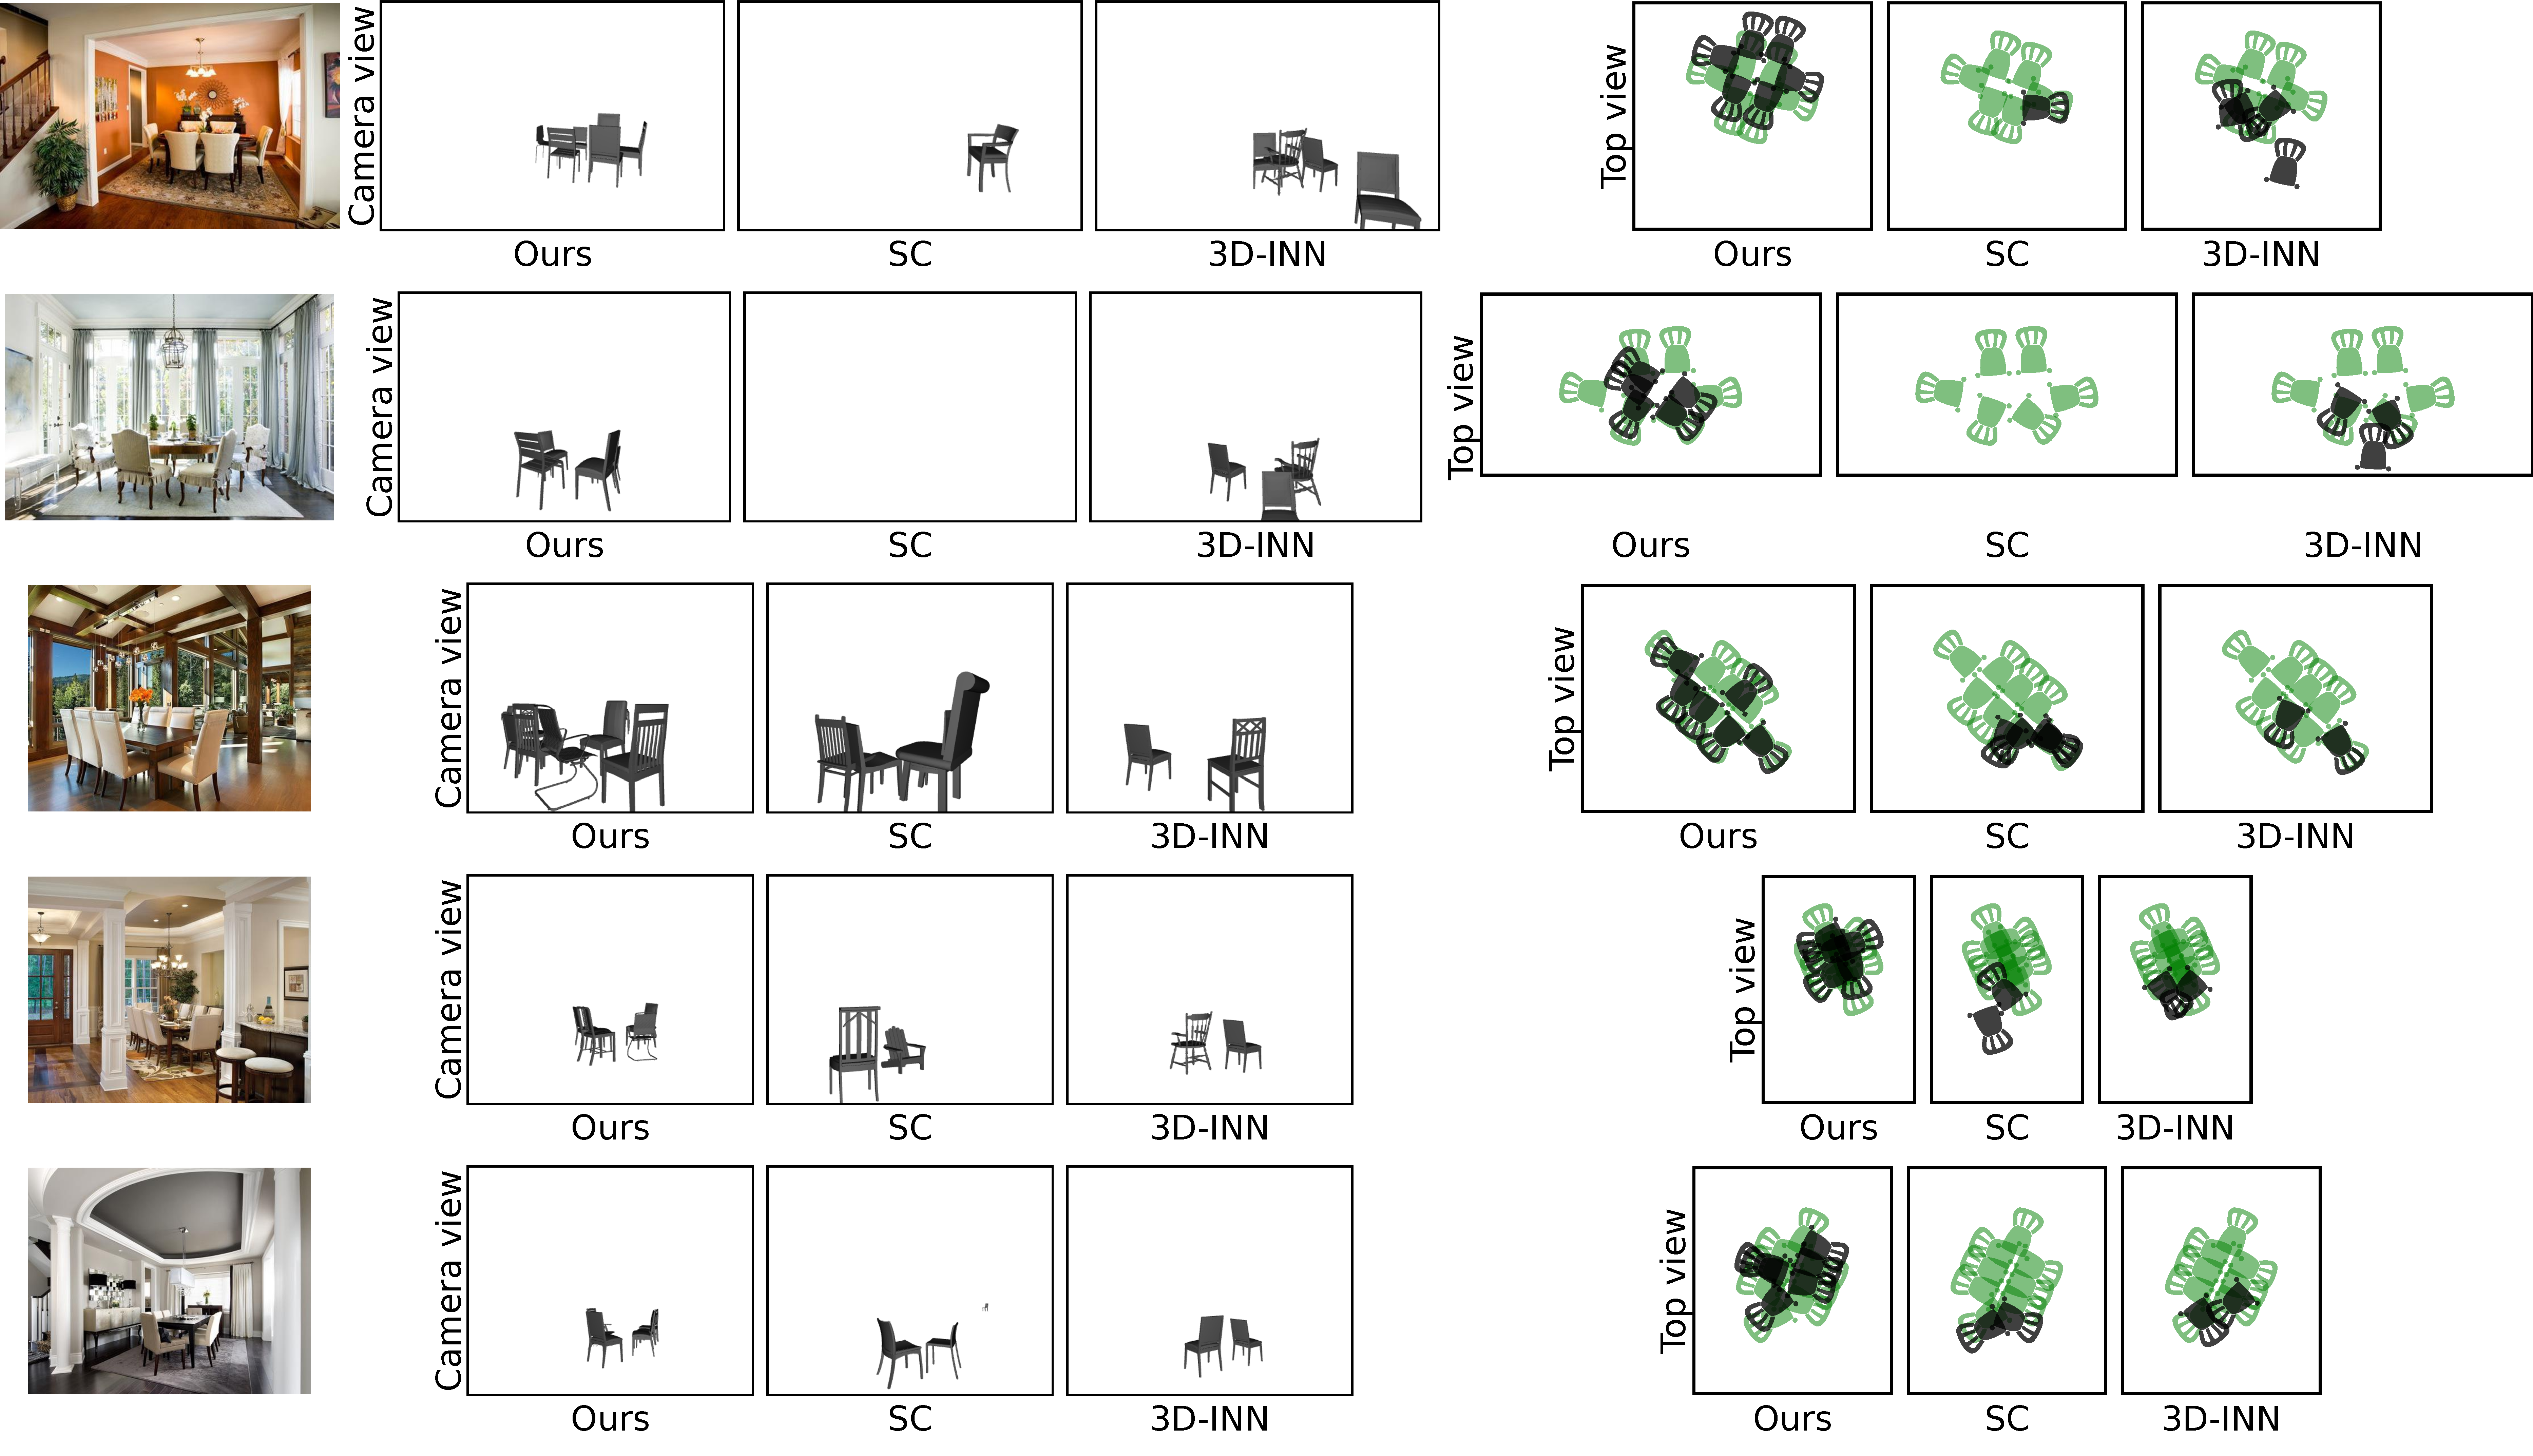
\includegraphics[width=\textwidth]{figures/qualitative_results/full/qual_results_16.pdf}
\end{sidewaysfigure}
\begin{sidewaysfigure}
    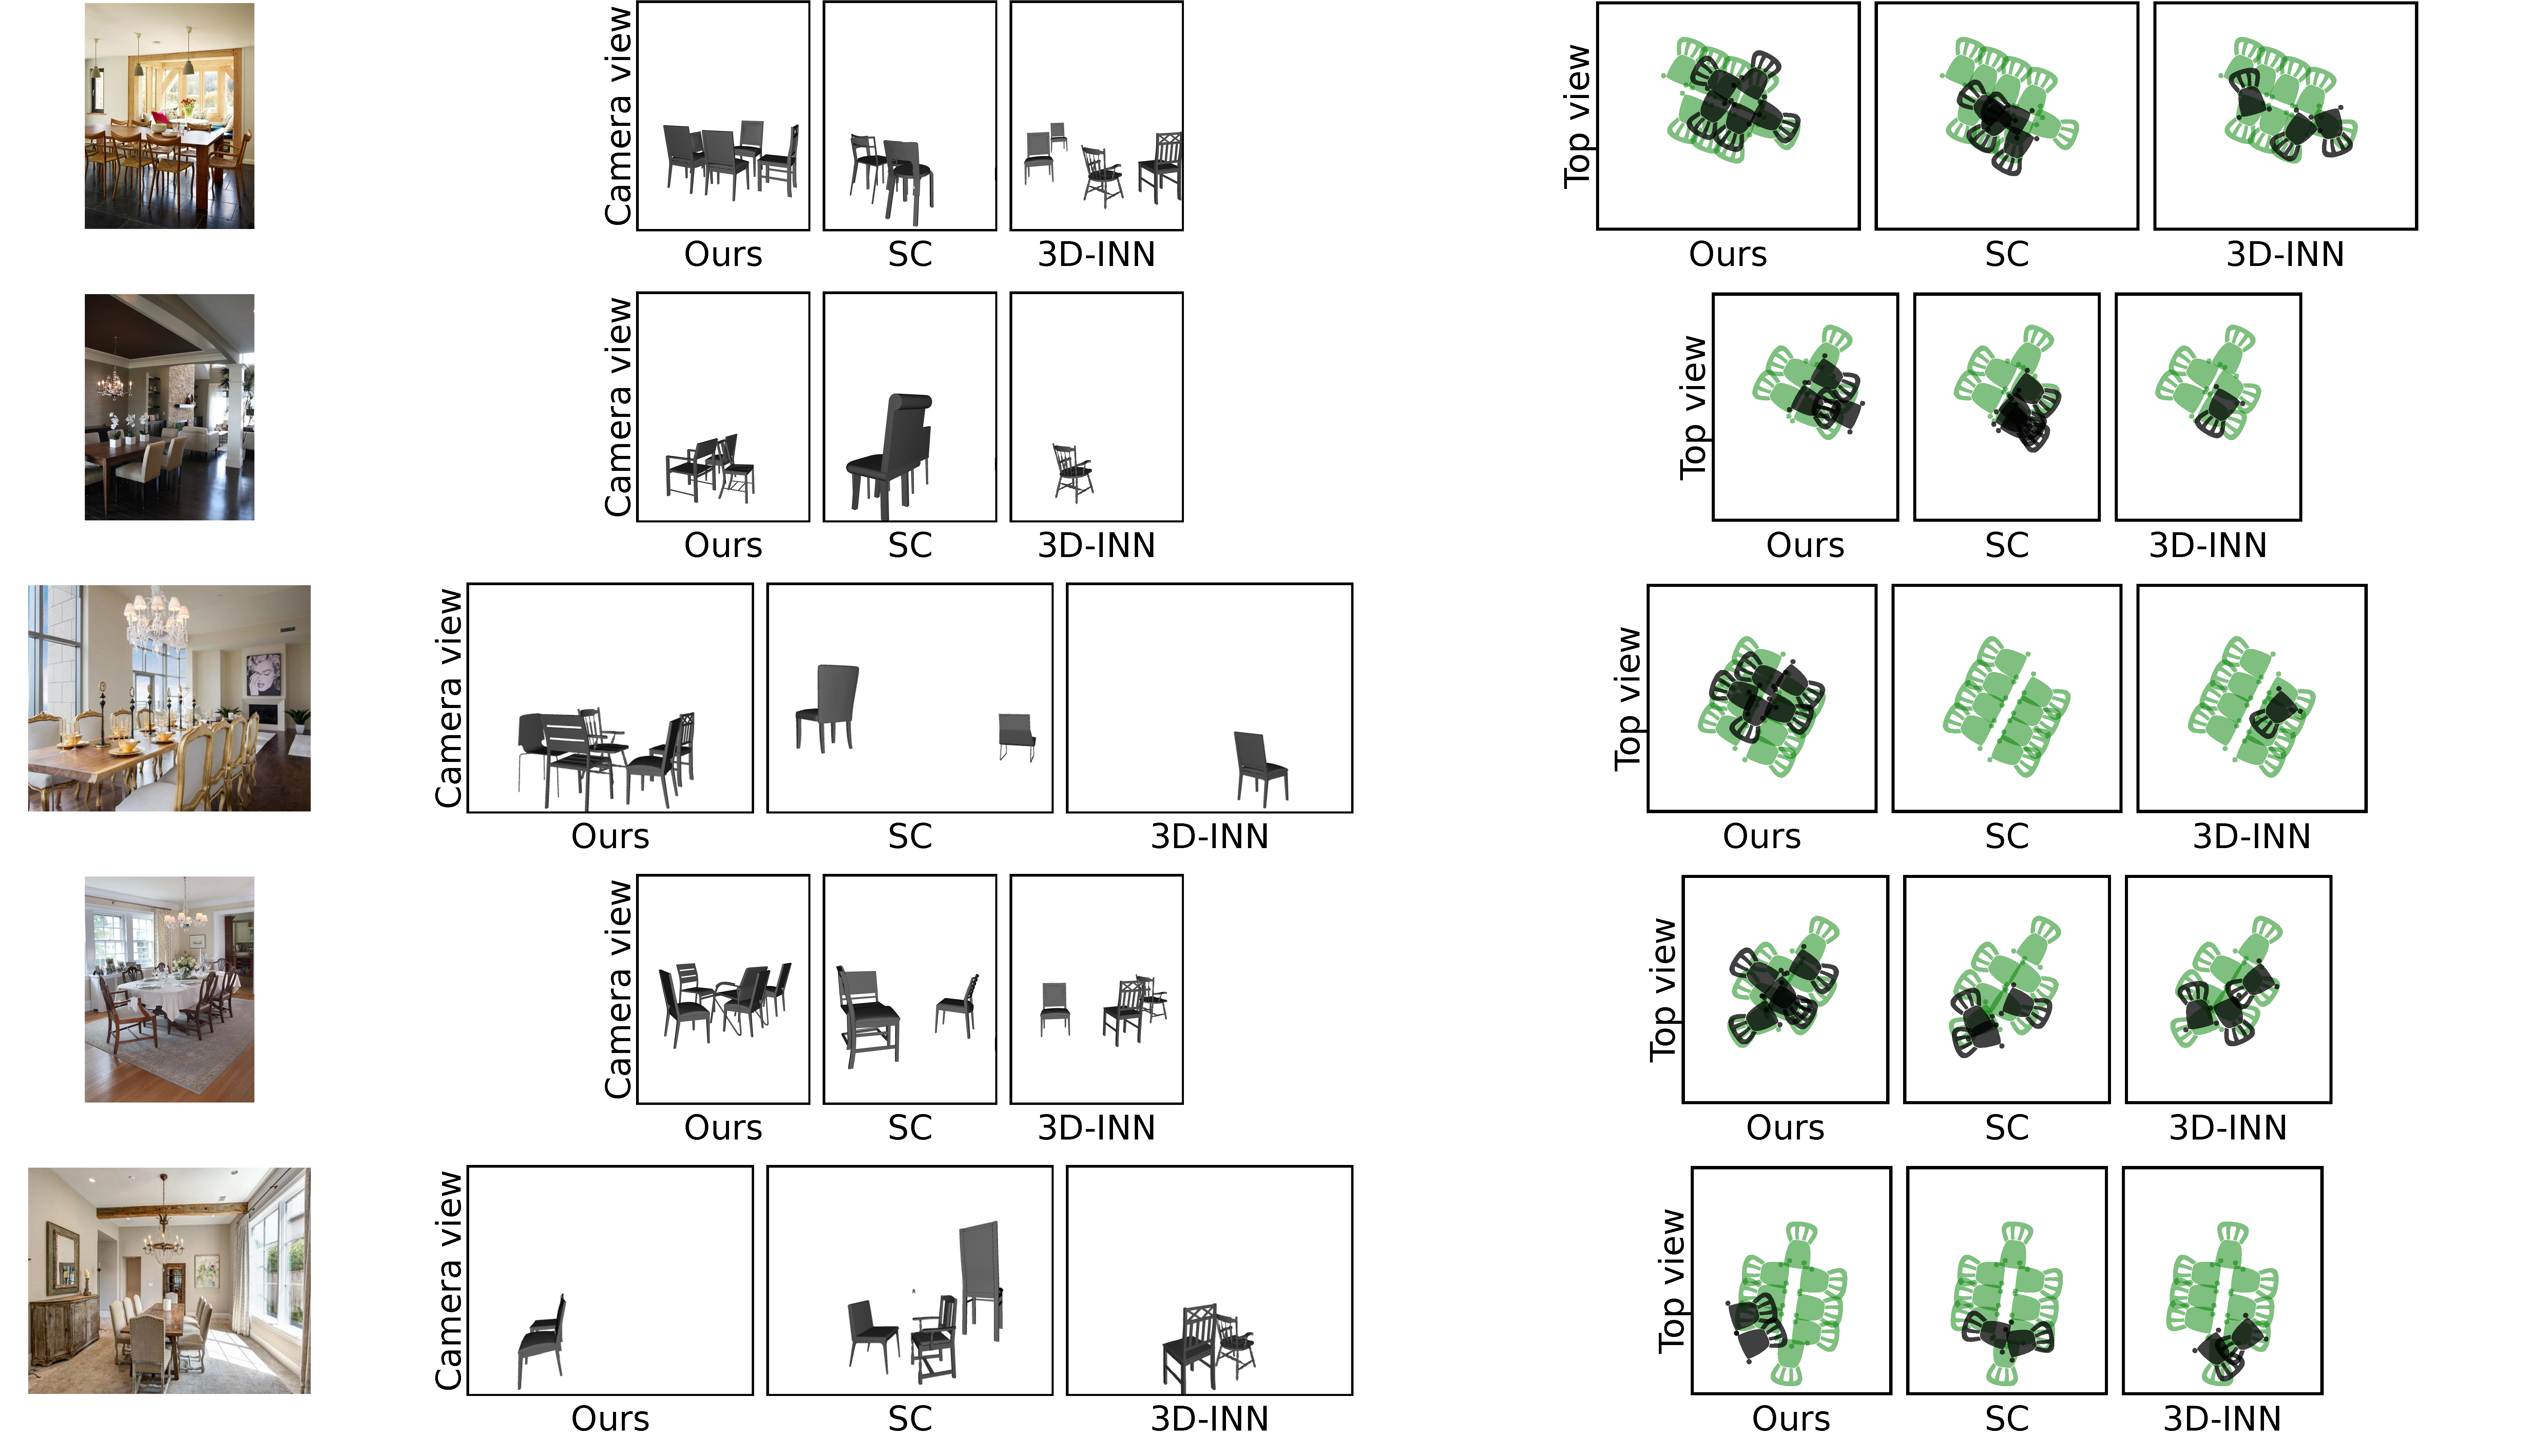
\includegraphics[width=\textwidth]{figures/qualitative_results/full/qual_results_17.pdf}
\end{sidewaysfigure}
\begin{sidewaysfigure}
    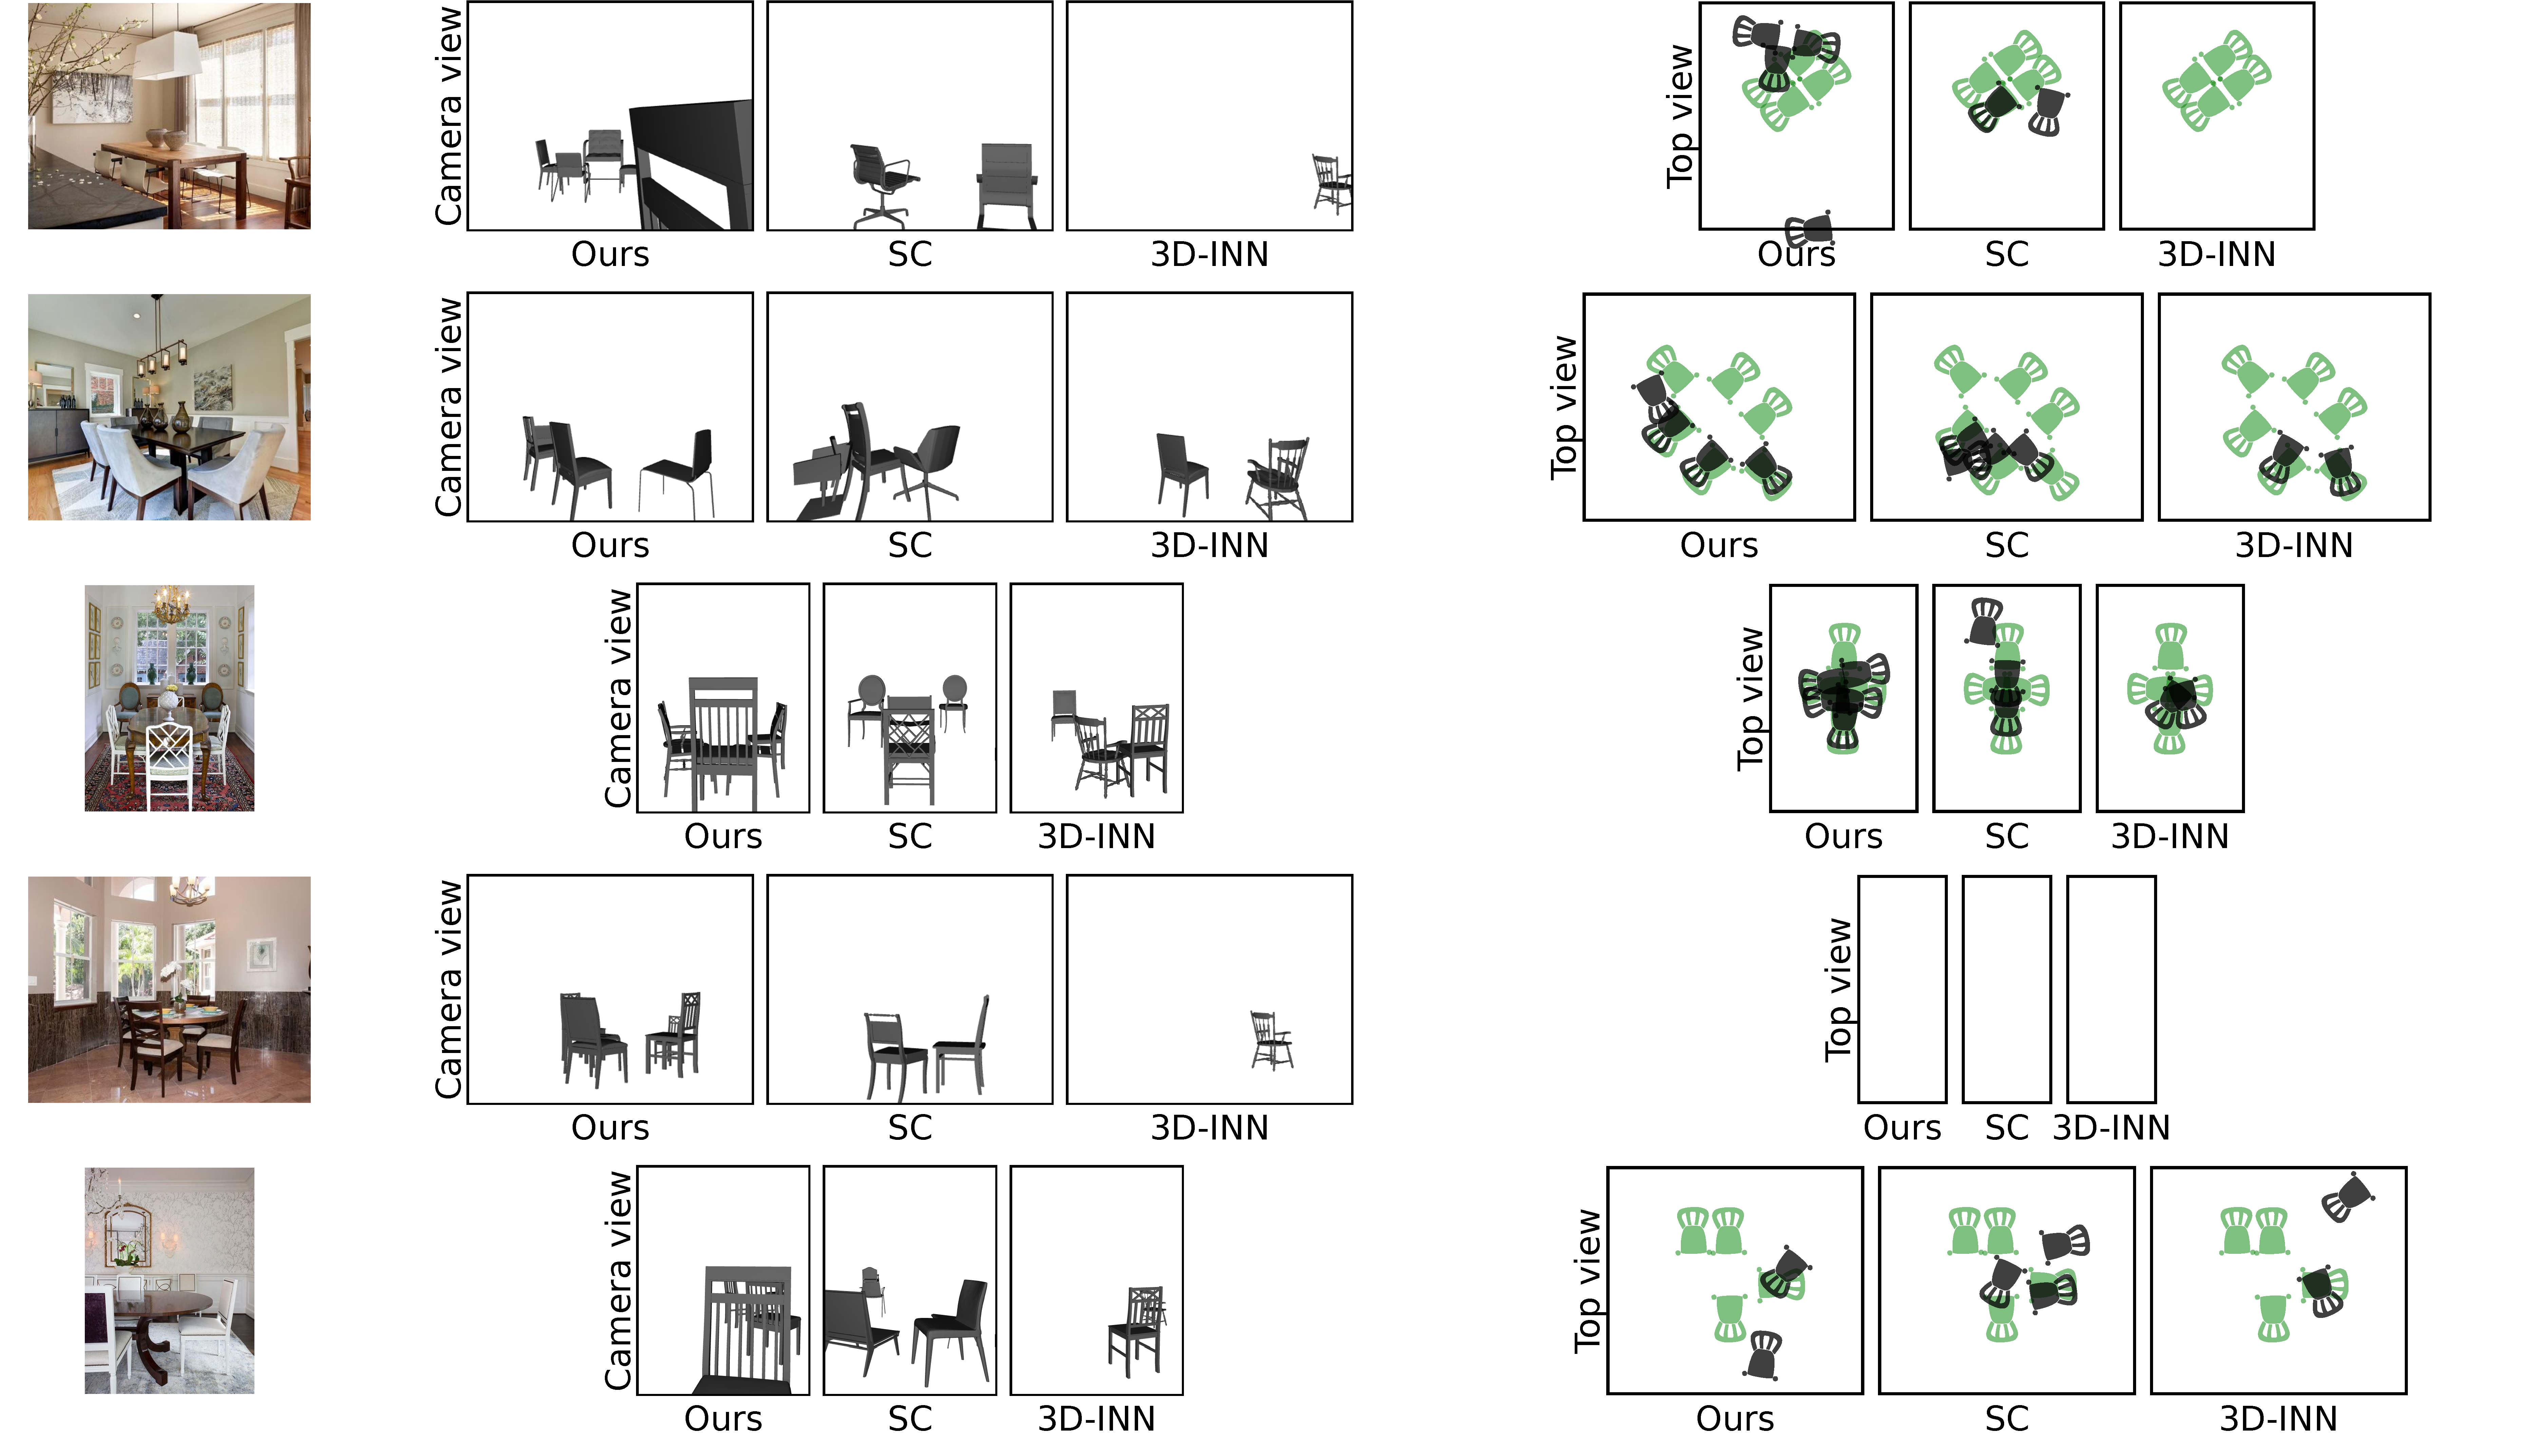
\includegraphics[width=\textwidth]{figures/qualitative_results/full/qual_results_18.pdf}
\end{sidewaysfigure}
\begin{sidewaysfigure}
    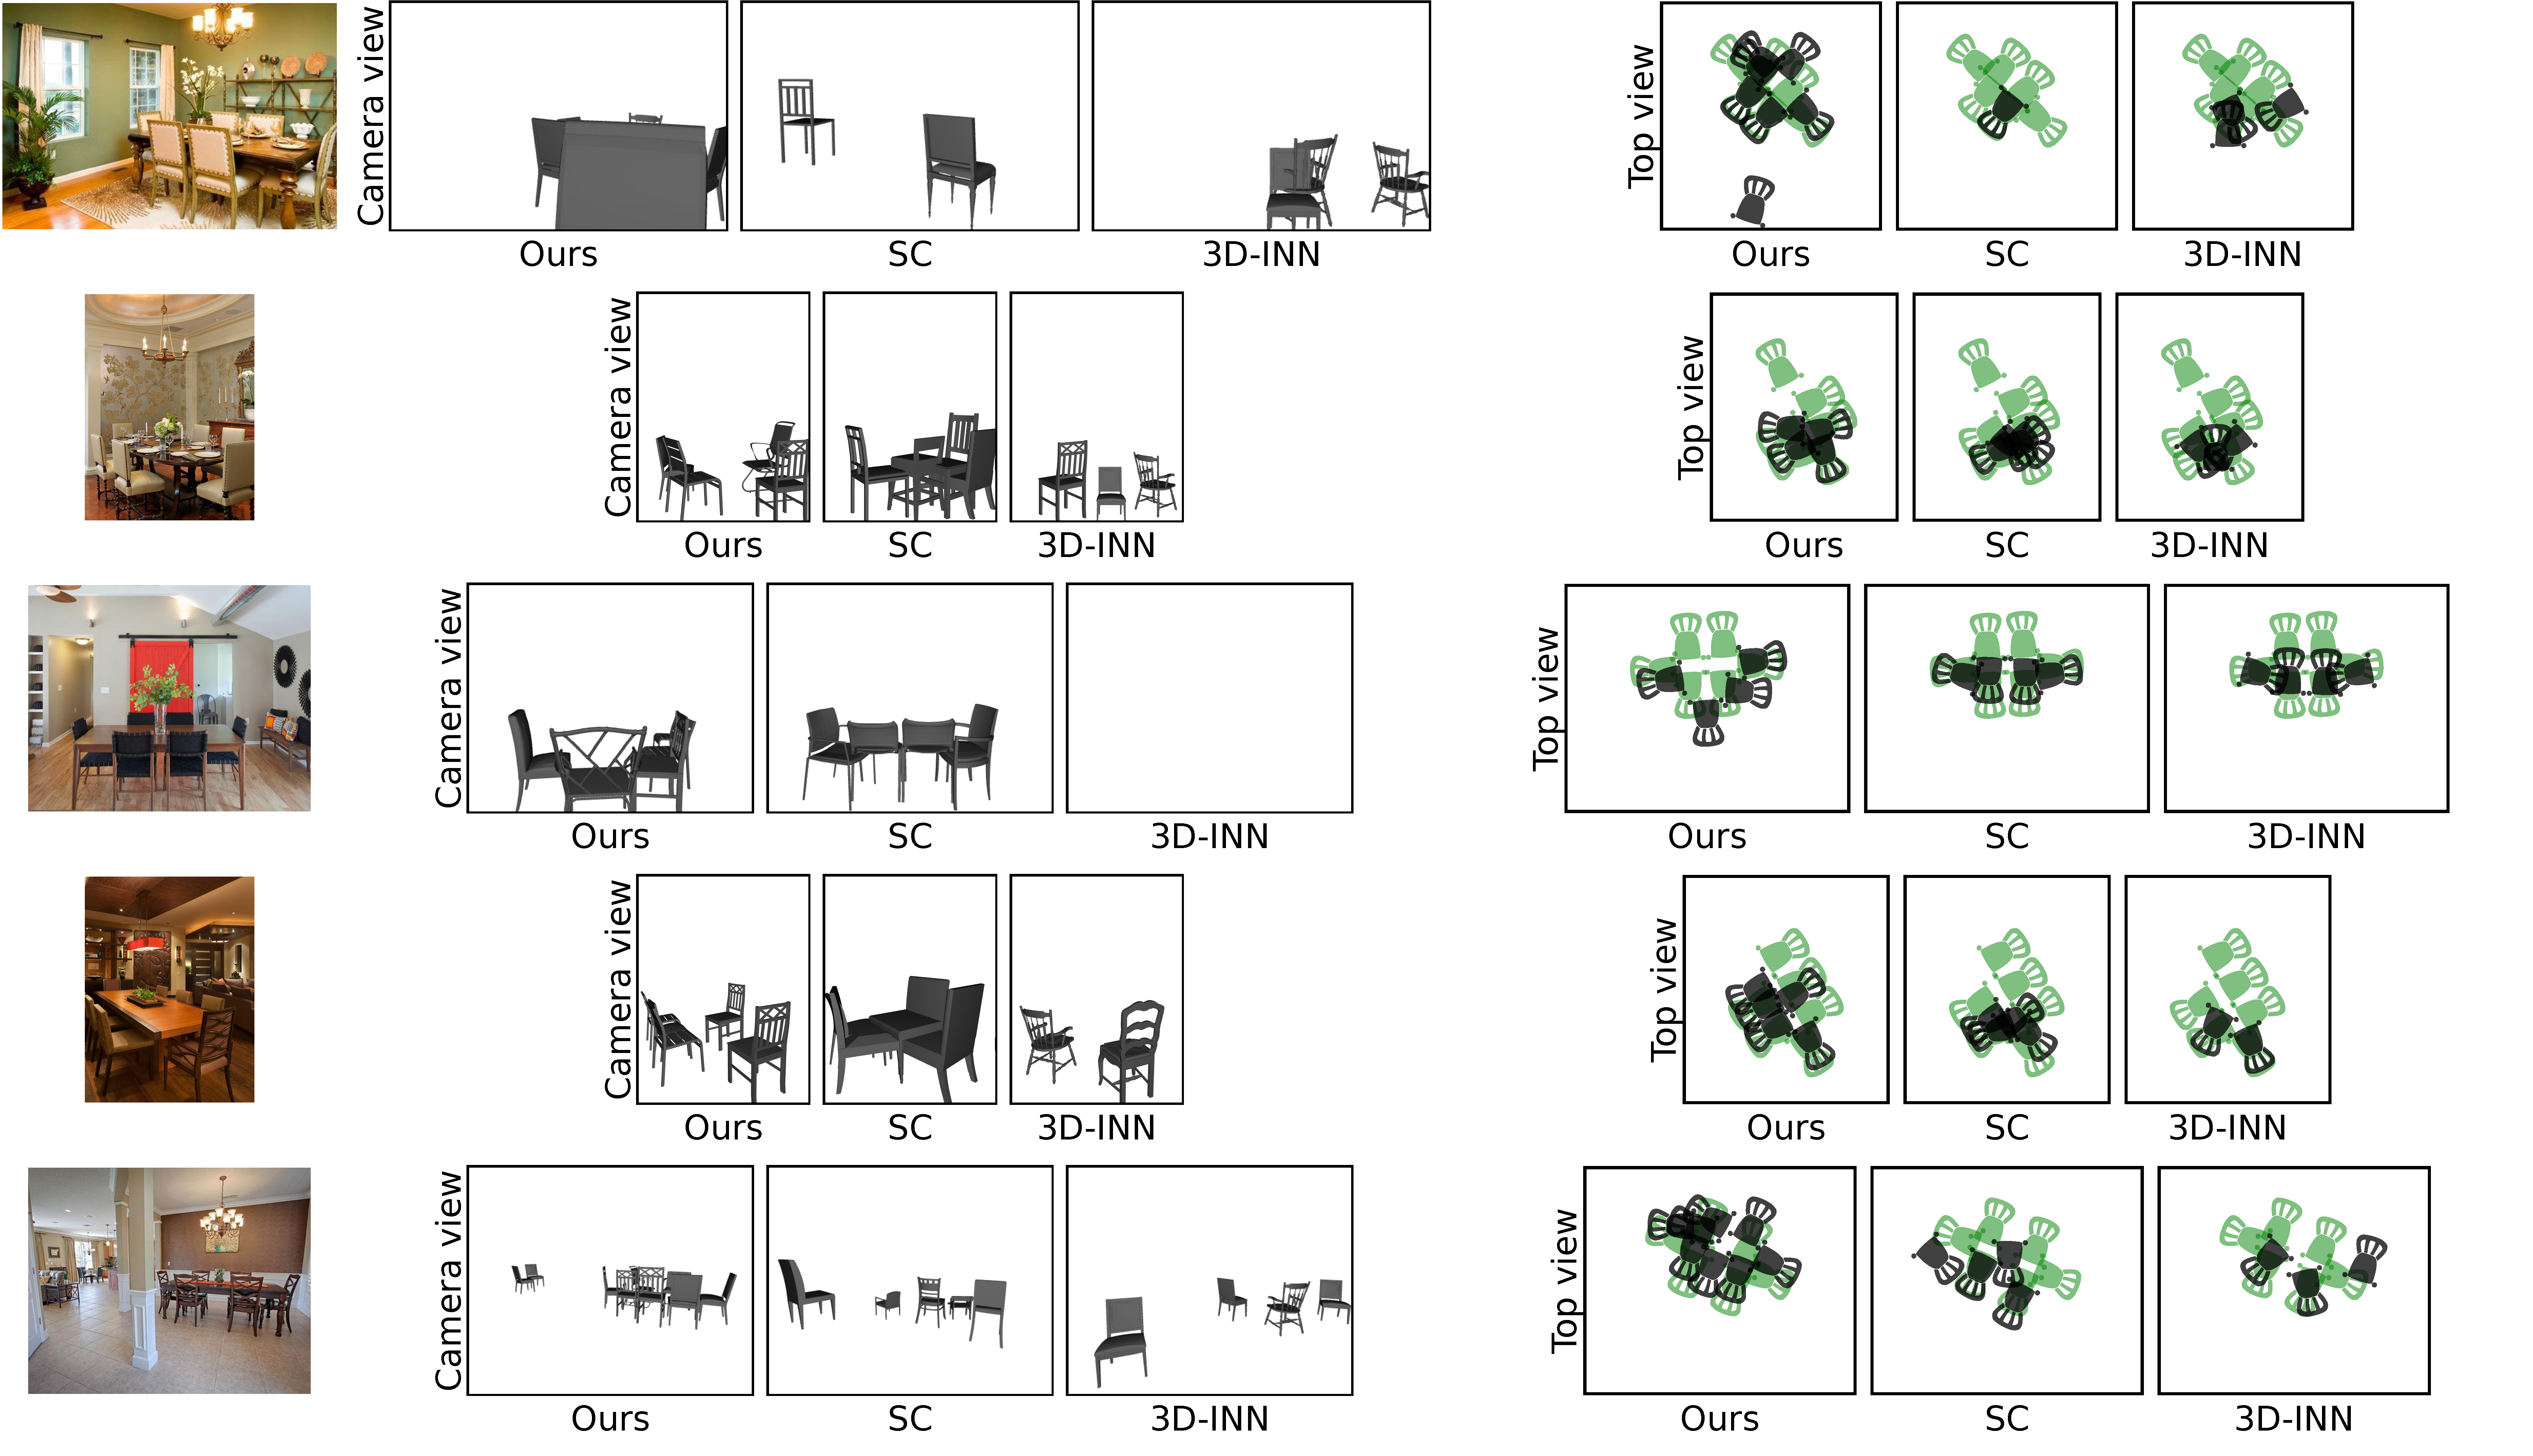
\includegraphics[width=\textwidth]{figures/qualitative_results/full/qual_results_19.pdf}
\end{sidewaysfigure}
\begin{sidewaysfigure}
    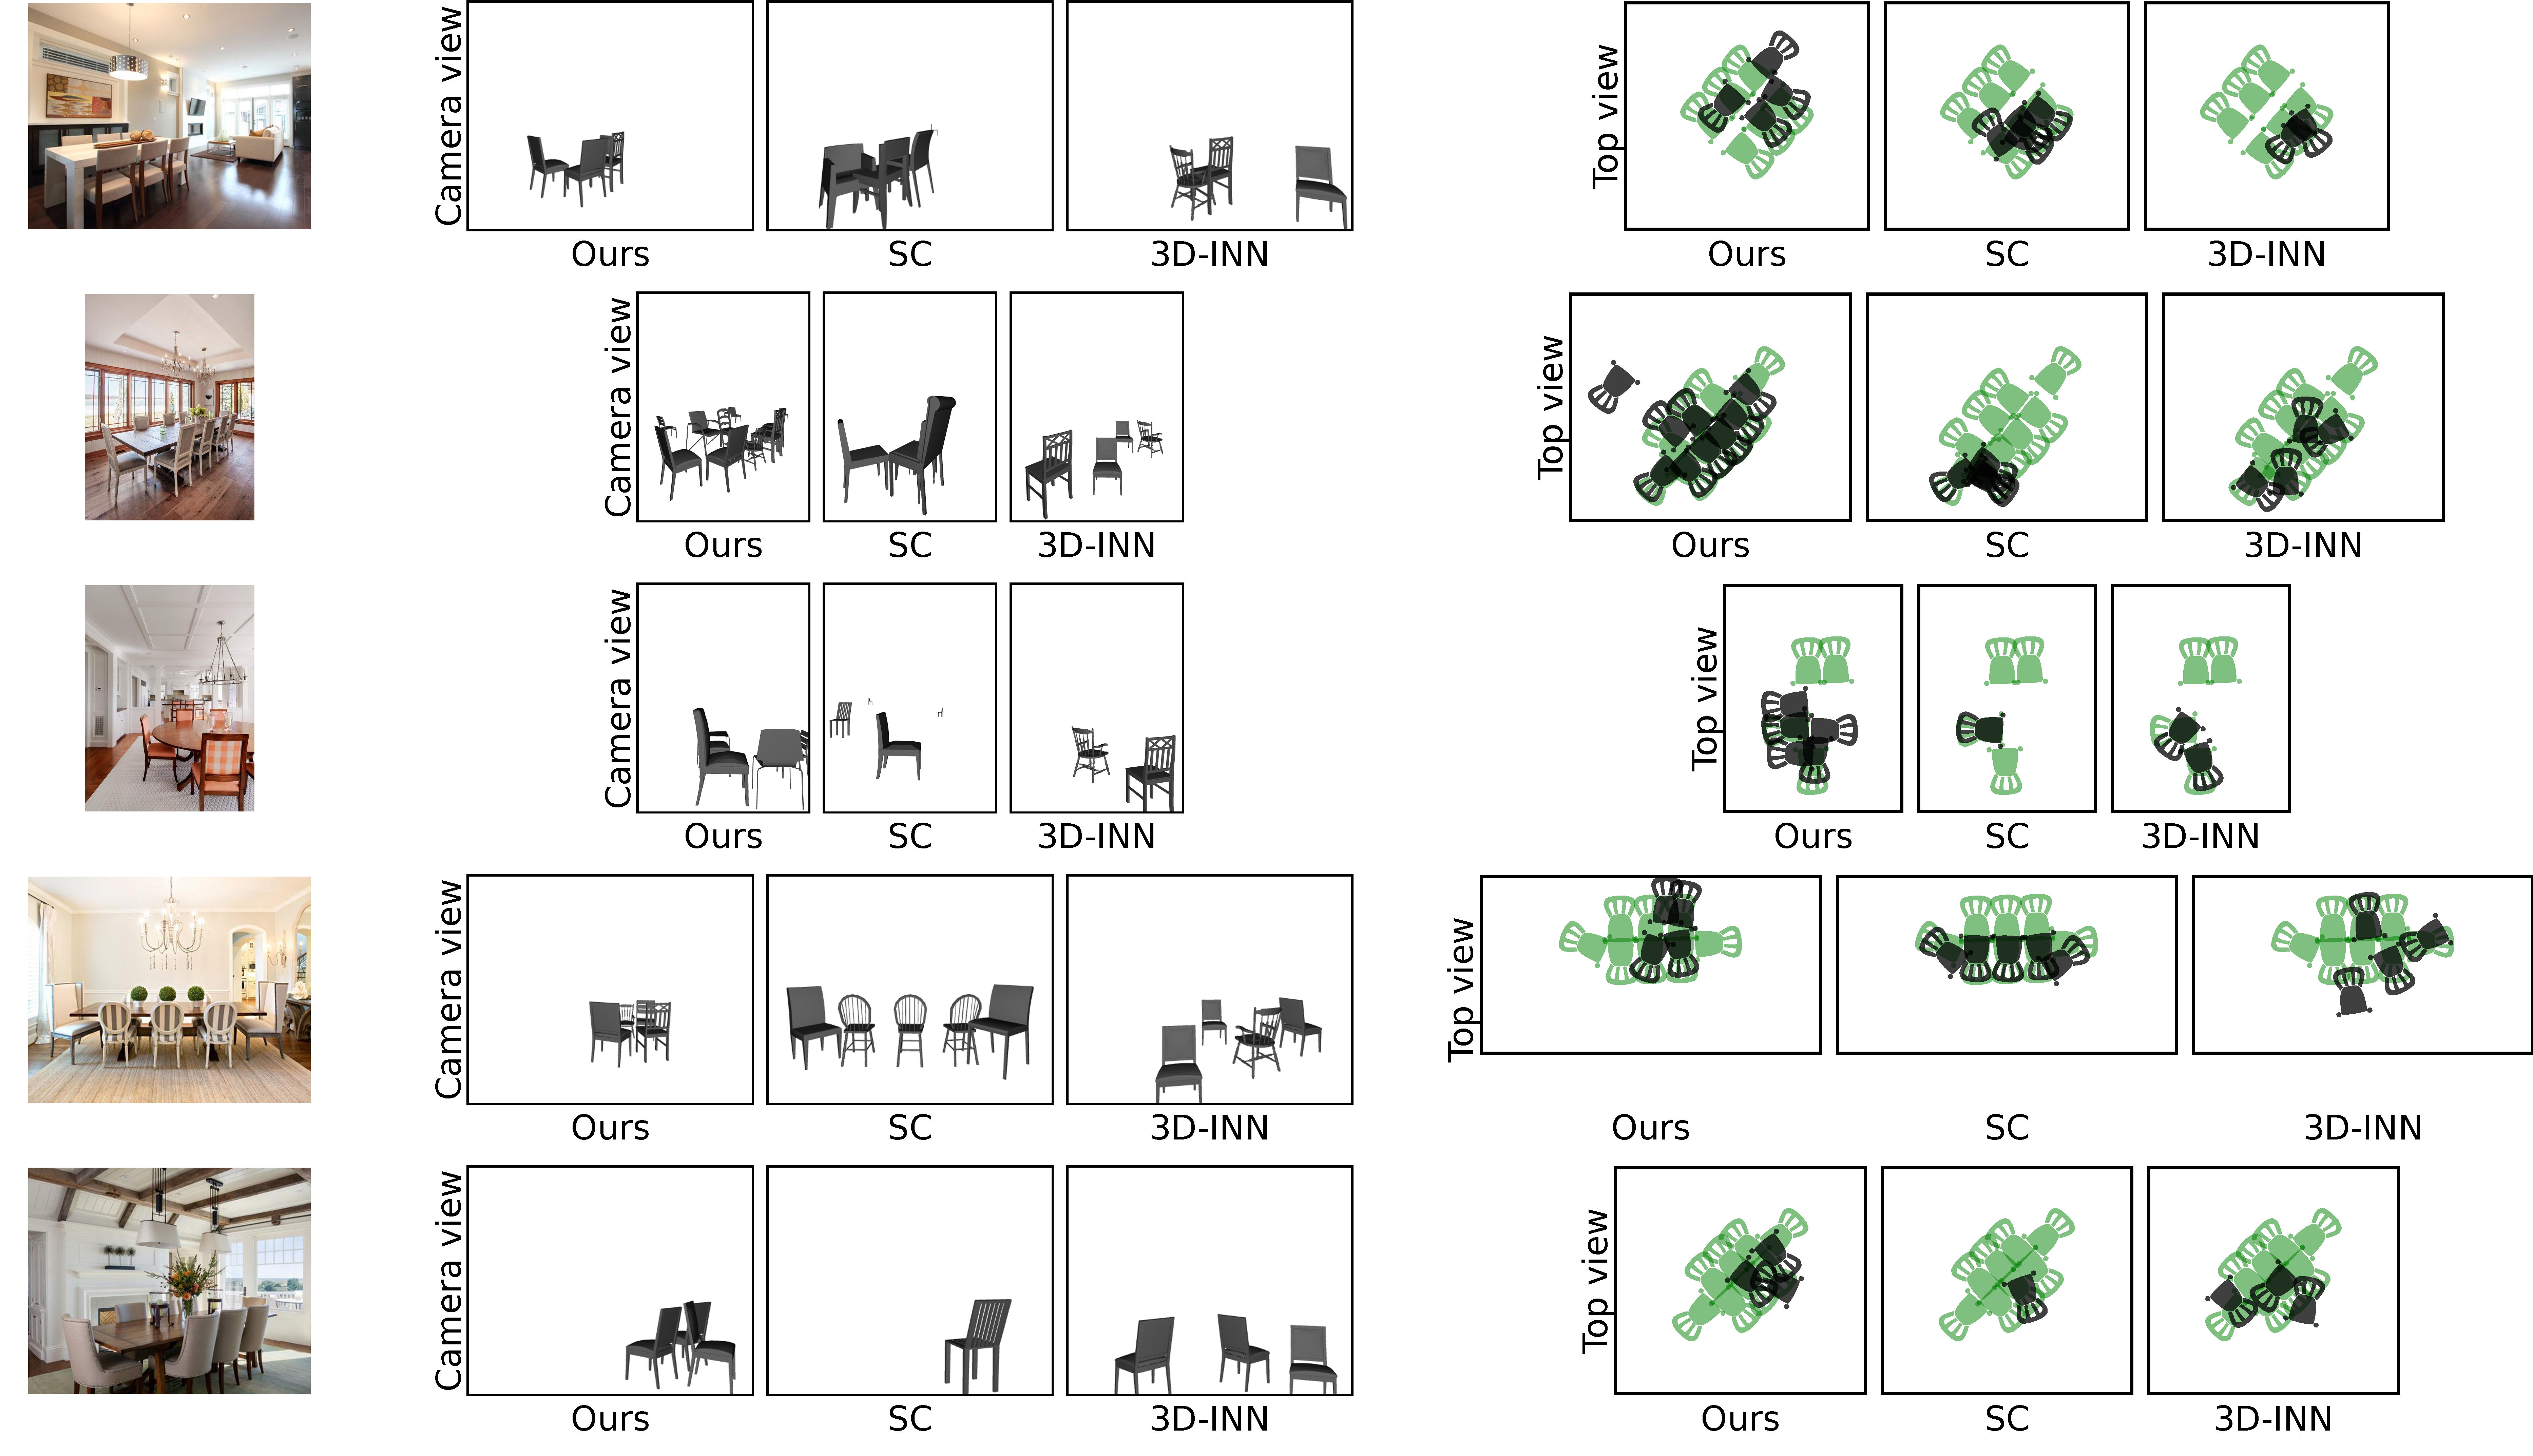
\includegraphics[width=\textwidth]{figures/qualitative_results/full/qual_results_20.pdf}
\end{sidewaysfigure}
\begin{sidewaysfigure}
    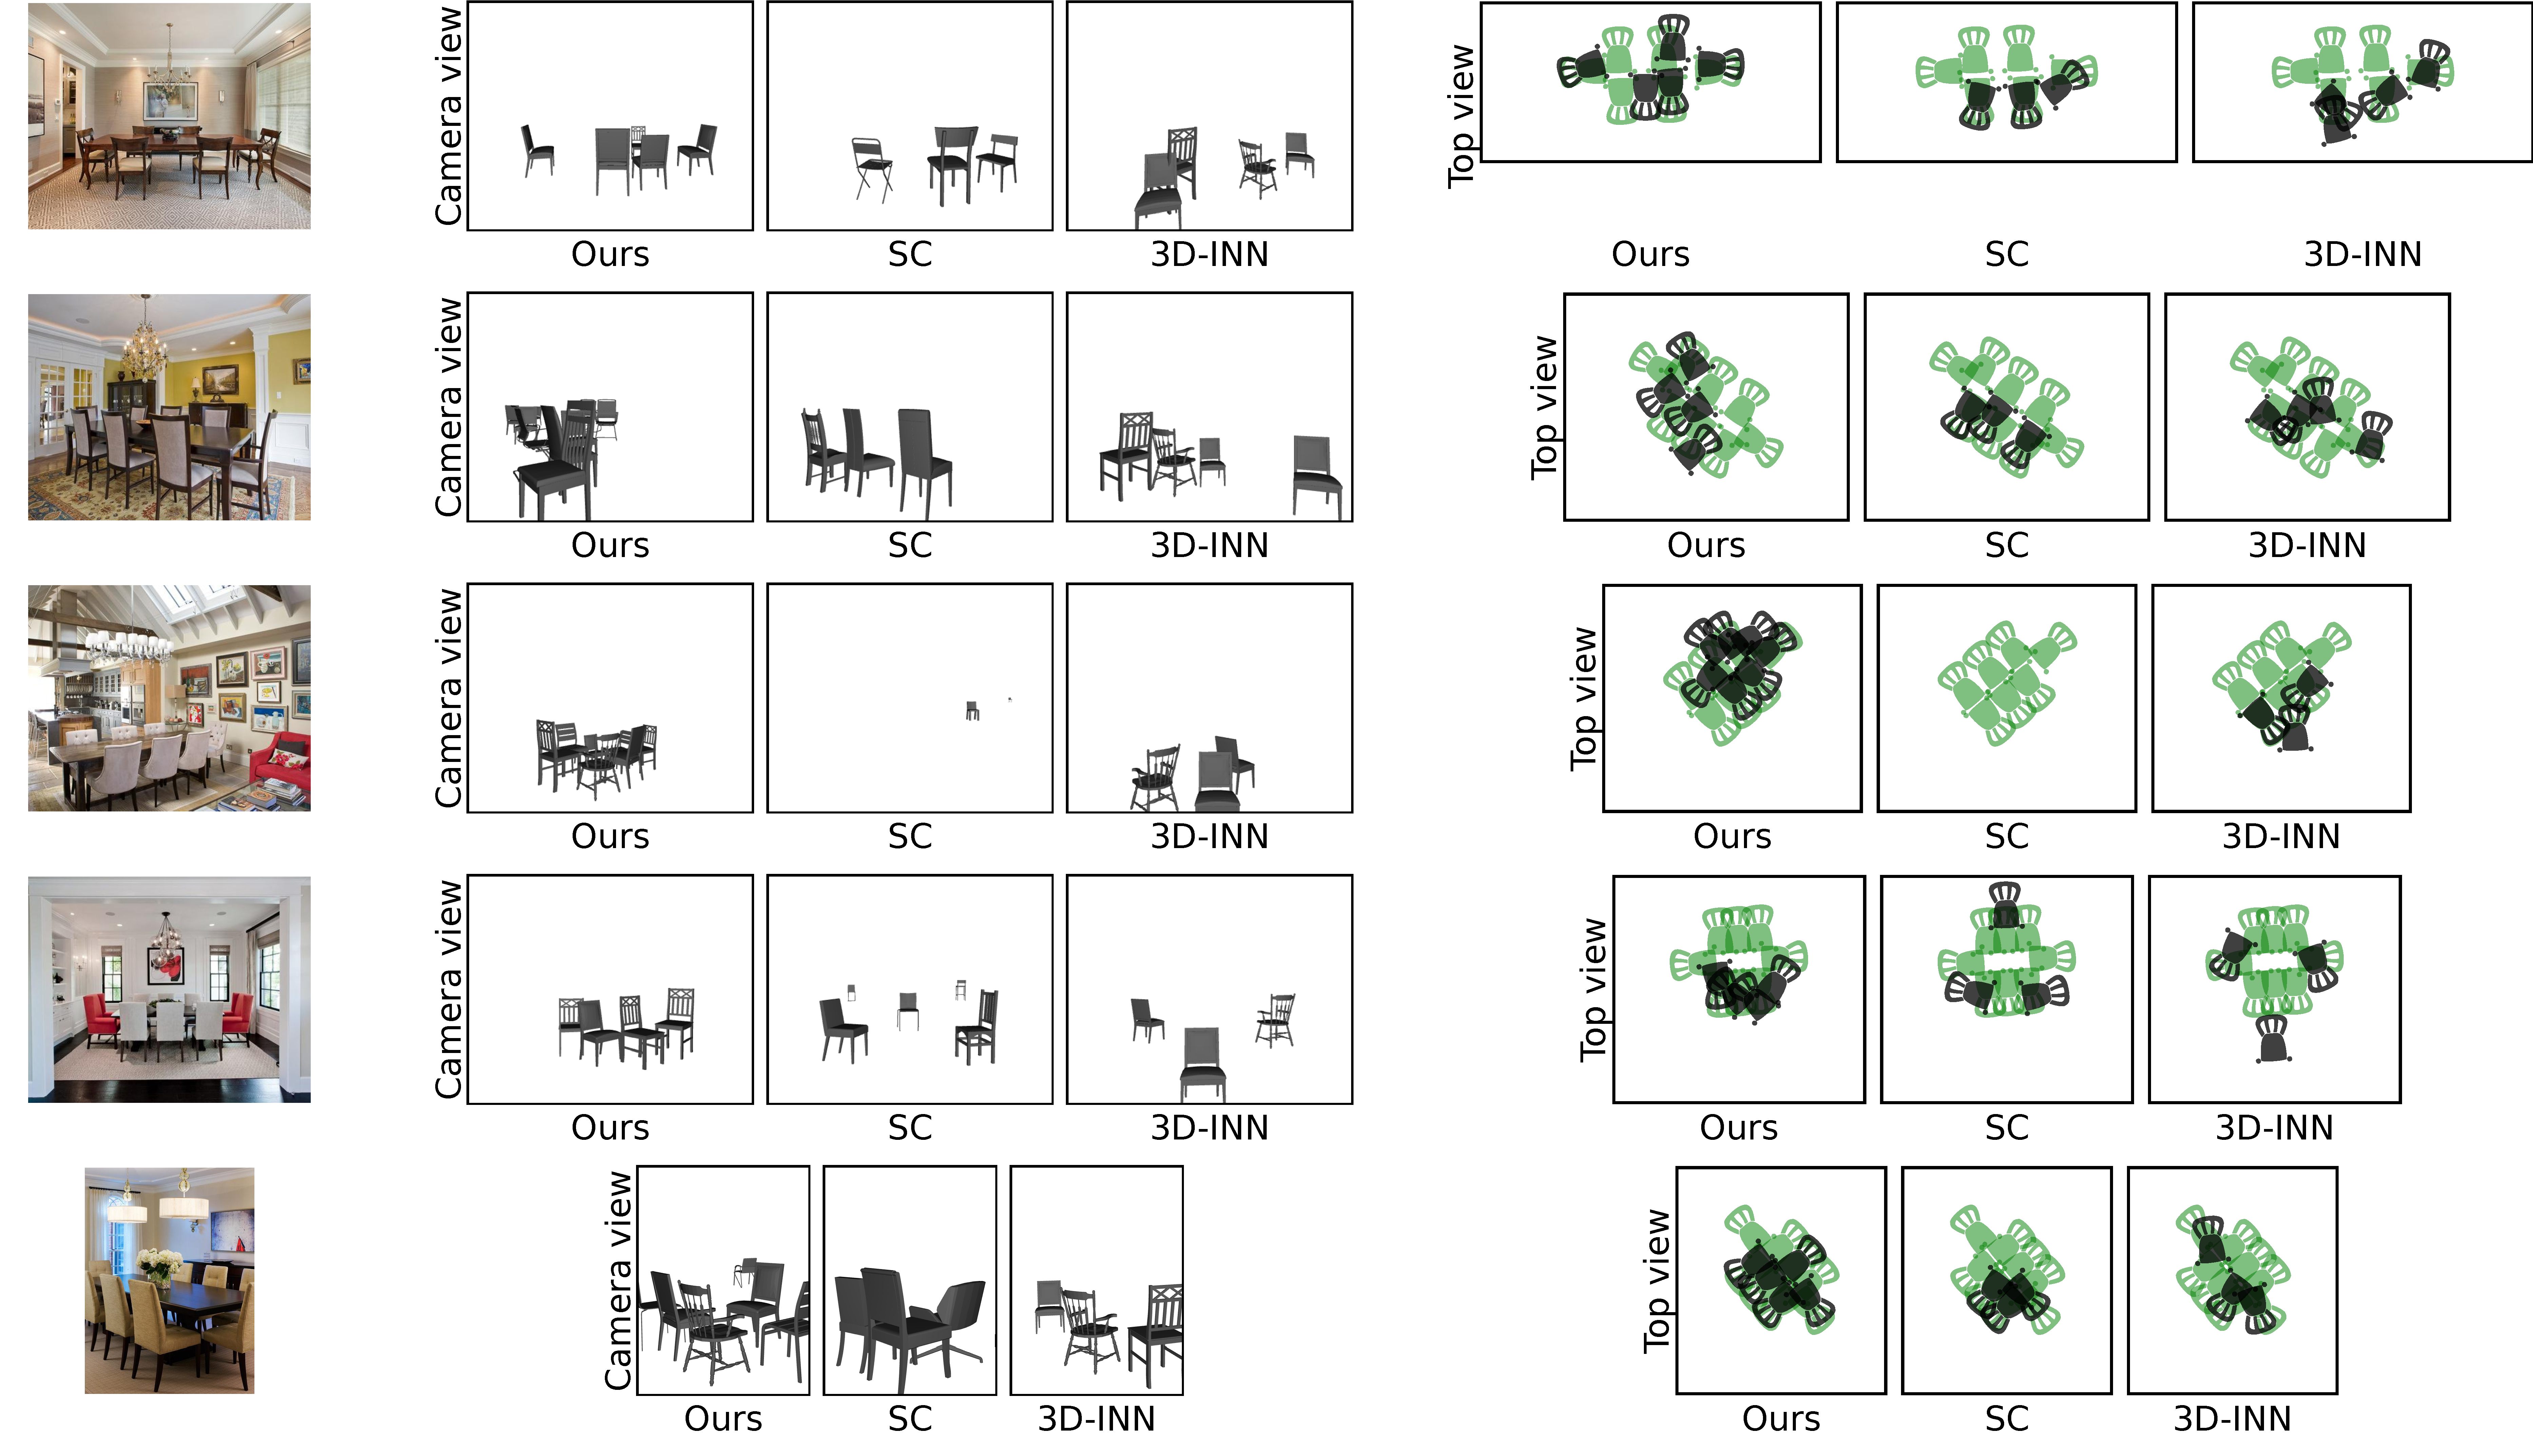
\includegraphics[width=\textwidth]{figures/qualitative_results/full/qual_results_21.pdf}
\end{sidewaysfigure}
\begin{sidewaysfigure}
    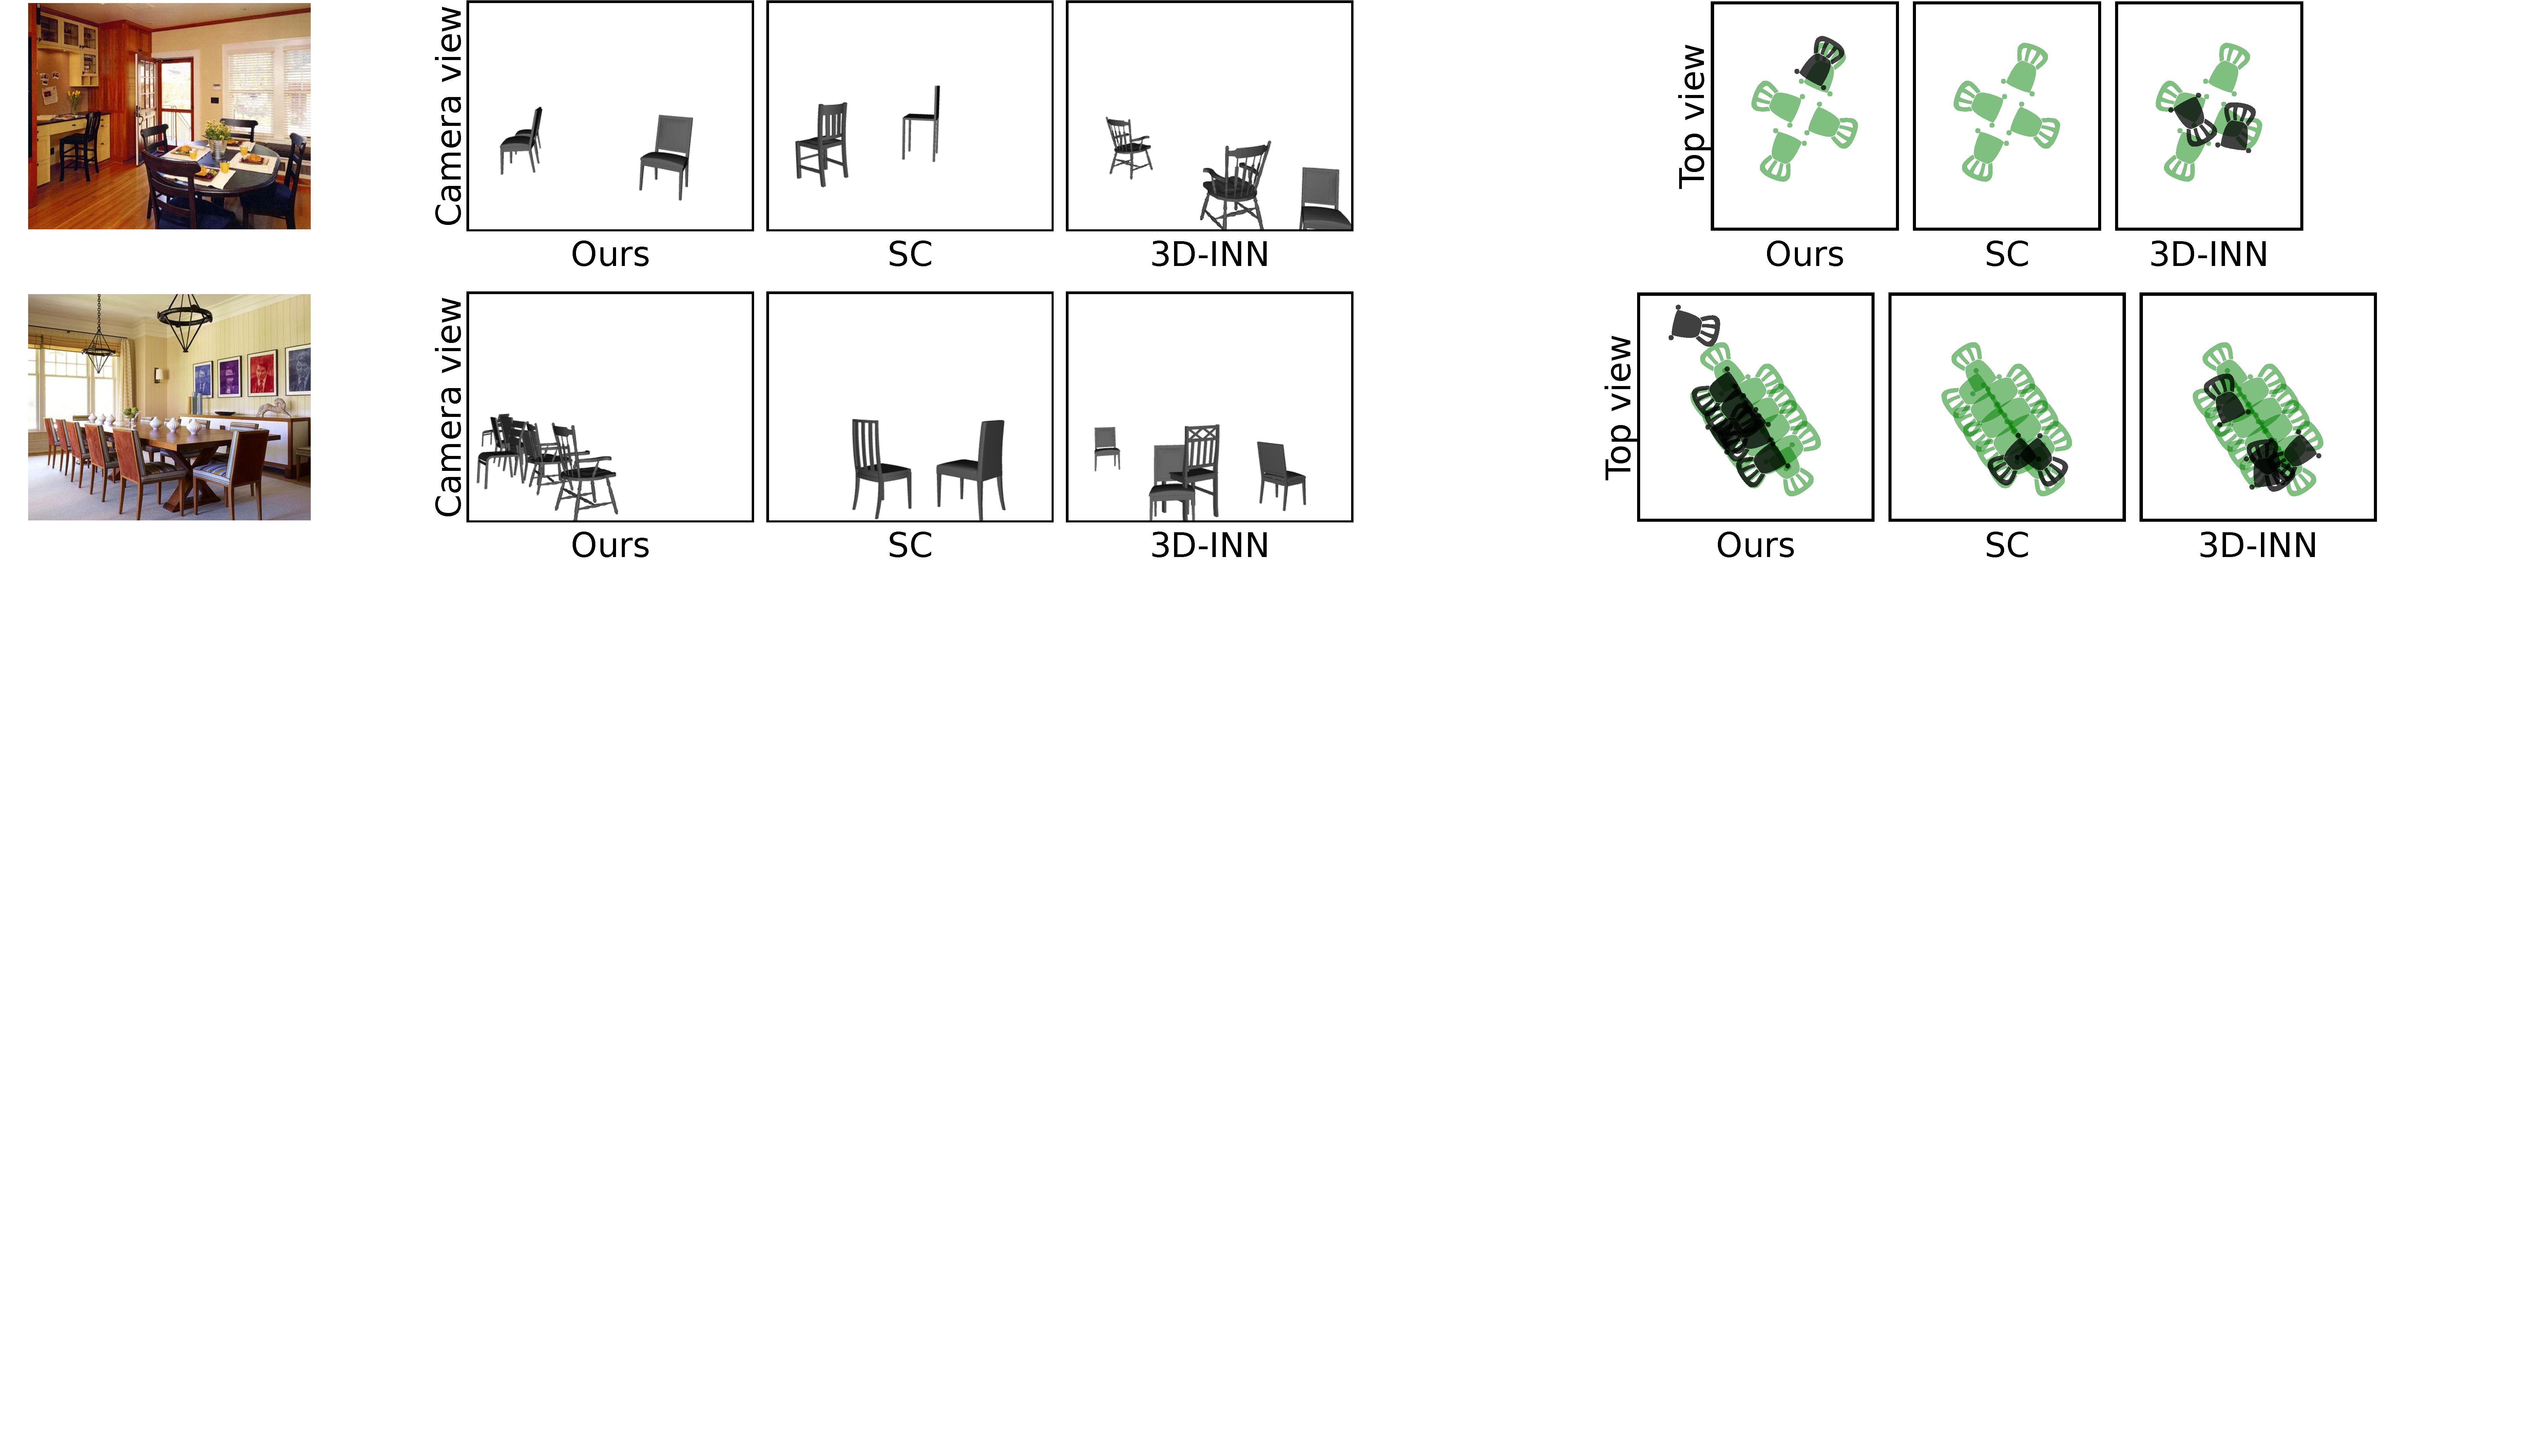
\includegraphics[width=\textwidth]{figures/qualitative_results/full/qual_results_22.pdf}
\end{sidewaysfigure}

\end{document}
